
\includegraphics[width=1in,height=0.54926in]{media/image2.png}

Build Your Own Blocks

8.0

\textsc{Snap\emph{!}} Reference Manual

\section{}\label{section}

\section[\hfill\break
Table of
Contents]{\texorpdfstring{\protect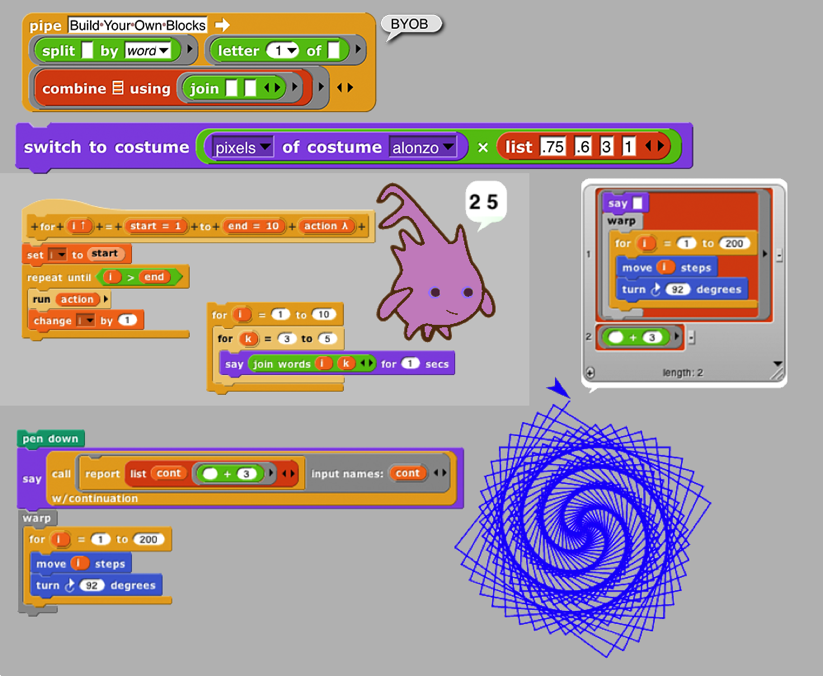
\includegraphics[width=5.47778in,height=4.50139in]{media/image3.png}\\
Table of Contents}{ Table of Contents}}\label{table-of-contents}

Brian Harvey

Jens Mönig

I. Blocks, Scripts, and Sprites \hyperref[blocks-scripts-and-sprites]{5}

Hat Blocks and Command Blocks
\hyperref[hat-blocks-and-command-blocks]{6}

A. Sprites and Parallelism \hyperref[sprites-and-parallelism]{8}

Costumes and Sounds \hyperref[costumes-and-sounds]{8}

Inter-Sprite Communication with Broadcast
\hyperref[inter-sprite-communication-with-broadcast]{9}

B. Nesting Sprites: Anchors and Parts
\hyperref[nesting-sprites-anchors-and-parts]{10}

C. Reporter Blocks and Expressions
\hyperref[reporter-blocks-and-expressions]{10}

D. Predicates and Conditional Evaluation
\hyperref[predicates-and-conditional-evaluation]{12}

E. Variables \hyperref[variables]{13}

Global Variables \hyperref[global-variables]{14}

Script Variables \hyperref[script-variables]{15}

Renaming variables \hyperref[renaming-variables]{15}

Transient variables \hyperref[transient-variables]{16}

F. Debugging \hyperref[debugging]{17}

The pause button \hyperref[the-pause-button]{17}

Breakpoints: the pause all block
\hyperref[breakpoints-the-pause-all-block]{17}

Visible stepping \hyperref[visible-stepping]{18}

G. Etcetera \hyperref[etcetera]{18}

H. Libraries \hyperref[libraries]{25}

II. Saving and Loading Projects and Media
\hyperref[saving-and-loading-projects-and-media]{37}

A. Local Storage \hyperref[local-storage]{37}

B. Creating a Cloud Account \hyperref[creating-a-cloud-account]{37}

C. Saving to the Cloud \hyperref[saving-to-the-cloud]{38}

D. Loading Saved Projects \hyperref[loading-saved-projects]{38}

E. \textbf{If you lose your project, do this first!}
\hyperref[if-you-lose-your-project-do-this-first]{39}

F. Private and Public Projects
\hyperref[private-and-public-projects]{39}

III. Building a Block \hyperref[building-a-block]{40}

A. Simple Blocks \hyperref[simple-blocks]{40}

Custom Blocks with Inputs \hyperref[custom-blocks-with-inputs]{42}

Editing Block Properties \hyperref[editing-block-properties]{43}

B. Recursion \hyperref[recursion]{43}

C. Block Libraries \hyperref[block-libraries]{44}

D. Custom blocks and Visible Stepping
\hyperref[custom-blocks-and-visible-stepping]{45}

IV. First class lists \hyperref[first-class-lists]{46}

A. The list Block \hyperref[the-list-block]{46}

B. Lists of Lists \hyperref[lists-of-lists]{47}

C. Functional and Imperative List Programming
\hyperref[functional-and-imperative-list-programming]{48}

D. Higher Order List Operations and Rings
\hyperref[higher-order-list-operations-and-rings]{49}

E. Table View vs. List View \hyperref[table-view-vs.-list-view]{51}

Comma-Separated Values \hyperref[comma-separated-values]{54}

Multi-dimensional lists and JSON
\hyperref[multi-dimensional-lists-and-json]{54}

F. Hyperblocks \hyperref[hyperblocks]{55}

V. Typed Inputs \hyperref[typed-inputs]{59}

A. Scratch's Type Notation \hyperref[scratchs-type-notation]{59}

B. The Snap! Input Type Dialog \hyperref[the-snap-input-type-dialog]{59}

Procedure Types \hyperref[procedure-types]{60}

Pulldown inputs
\hyperref[macintosh-hdusersbhdesktopgear-part.pngpulldown-inputs]{61}

Input variants \hyperref[input-variants]{63}

Prototype Hints \hyperref[prototype-hints]{64}

Title Text and Symbols \hyperref[title-text-and-symbols]{64}

VI. Procedures as Data \hyperref[procedures-as-data]{65}

A. Call and Run \hyperref[call-and-run]{65}

Call/Run with inputs \hyperref[callrun-with-inputs]{65}

Variables in Ring Slots \hyperref[variables-in-ring-slots]{66}

B. Writing Higher Order Procedures
\hyperref[writing-higher-order-procedures]{66}

Recursive Calls to Multiple-Input Blocks
\hyperref[recursive-calls-to-multiple-input-blocks]{68}

C. Formal Parameters \hyperref[formal-parameters]{69}

D. Procedures as Data \hyperref[procedures-as-data-1]{70}

E. Special Forms \hyperref[special-forms]{71}

Special Forms in Scratch \hyperref[special-forms-in-scratch]{72}

VII. Object Oriented Programming with Sprites
\hyperref[object-oriented-programming-with-sprites]{73}

A. First Class Sprites \hyperref[first-class-sprites]{73}

B. Permanent and Temporary Clones
\hyperref[permanent-and-temporary-clones]{74}

C. Sending Messages to Sprites
\hyperref[sending-messages-to-sprites]{74}

Polymorphism \hyperref[polymorphism]{75}

D. Local State in Sprites: Variables and Attributes
\hyperref[local-state-in-sprites-variables-and-attributes]{76}

E. Prototyping: Parents and Children
\hyperref[prototyping-parents-and-children]{76}

F. Inheritance by Delegation \hyperref[inheritance-by-delegation]{77}

G. List of attributes \hyperref[attrib.pnglist-of-attributes]{78}

H. First Class Costumes and Sounds
\hyperref[first-class-costumes-and-sounds]{79}

Media Computation with Costumes
\hyperref[media-computation-with-costumes]{79}

Media Computation with Sounds
\hyperref[media-computation-with-sounds]{82}

VIII. OOP with Procedures \hyperref[oop-with-procedures]{85}

A. Local State with Script Variables
\hyperref[local-state-with-script-variables]{85}

B. Messages and Dispatch Procedures
\hyperref[messages-and-dispatch-procedures]{86}

C. Inheritance via Delegation \hyperref[inheritance-via-delegation]{87}

D. An Implementation of Prototyping OOP
\hyperref[an-implementation-of-prototyping-oop]{88}

IX. The Outside World \hyperref[the-outside-world]{91}

A. The World Wide Web \hyperref[the-world-wide-web]{91}

B. Hardware Devices \hyperref[hardware-devices]{92}

C. Date and Time \hyperref[date-and-time]{92}

X. Continuations \hyperref[continuations]{93}

A. Continuation Passing Style \hyperref[continuation-passing-style]{94}

B. Call/Run w/Continuation \hyperref[callrun-wcontinuation]{97}

Nonlocal exit \hyperref[nonlocal-exit]{99}

XI. Metaprogramming \hyperref[metaprogramming]{101}

A. Reading a block \hyperref[reading-a-block]{101}

B. Writing a block \hyperref[writing-a-block]{102}

C. Macros \hyperref[macros]{105}

XII. User Interface Elements \hyperref[user-interface-elements]{107}

A. Tool Bar Features \hyperref[tool-bar-features]{107}

The Snap\emph{!} Logo Menu \hyperref[the-snap-logo-menu]{107}

The File Menu \hyperref[the-file-menu]{108}

The Cloud Menu \hyperref[the-cloud-menu]{113}

The Settings Menu \hyperref[the-settings-menu]{114}

Visible Stepping Controls \hyperref[visible-stepping-controls]{117}

Stage Resizing Buttons \hyperref[stage-resizing-buttons]{118}

Project Control Buttons \hyperref[project-control-buttons]{118}

B. The Palette Area \hyperref[the-palette-area]{119}

Buttons in the Palette \hyperref[buttons-in-the-palette]{119}

Context Menus for Palette Blocks
\hyperref[context-menus-for-palette-blocks]{119}

Context Menu for the Palette Background
\hyperref[context-menu-for-the-palette-background]{120}

C. The Scripting Area \hyperref[the-scripting-area]{122}

Sprite Appearance and Behavior Controls
\hyperref[sprite-appearance-and-behavior-controls]{122}

Scripting Area Tabs \hyperref[scripting-area-tabs]{122}

Scripts and Blocks Within Scripts
\hyperref[scripts-and-blocks-within-scripts]{122}

Controls in the Costumes Tab
\hyperref[controls-in-the-costumes-tab]{126}

The Paint Editor \hyperref[the-paint-editor]{128}

Controls in the Sounds Tab \hyperref[controls-in-the-sounds-tab]{130}

D. Keyboard Editing \hyperref[keyboard-editing]{130}

Starting and stopping the keyboard editor
\hyperref[starting-and-stopping-the-keyboard-editor]{130}

Navigating in the keyboard editor
\hyperref[navigating-in-the-keyboard-editor]{130}

Editing a script \hyperref[editing-a-script]{131}

Running the selected script \hyperref[running-the-selected-script]{132}

E. Controls on the Stage \hyperref[controls-on-the-stage]{132}

Sprites \hyperref[sprites]{132}

Variable watchers
\hyperref[macintosh-hdusersbhdesktopwatcher-menu.pngvariable-watchers]{134}

The stage itself \hyperref[the-stage-itself]{135}

F. The Sprite Corral and Sprite Creation Buttons
\hyperref[the-sprite-corral-and-sprite-creation-buttons]{135}

G. Preloading a Project when Starting Snap!
\hyperref[preloading-a-project-when-starting-snap]{136}

H. Mirror Sites \hyperref[mirror-sites]{137}

Appendix A. Snap\emph{!} color library
\hyperref[appendix-a.-snap-color-library]{138}

Introduction to Color \hyperref[introduction-to-color]{138}

Crayons and Color Numbers \hyperref[crayons-and-color-numbers]{139}

Perceptual Spaces: HSV and HSL
\hyperref[perceptual-spaces-hsv-and-hsl]{142}

Mixing Colors \hyperref[mixing-colors]{144}

tl;dr \hyperref[tldr]{145}

Subappendix: Geeky details on fair hue
\hyperref[subappendix-geeky-details-on-fair-hue]{145}

Subappendix: Geeky details on color numbers
\hyperref[subappendix-geeky-details-on-color-numbers]{146}

Appendix B. APL features \hyperref[appendix-b.-apl-features]{148}

Boolean values \hyperref[boolean-values]{150}

Scalar functions \hyperref[scalar-functions]{150}

Mixed functions \hyperref[mixed-functions]{151}

Higher order functions \hyperref[higher-order-functions]{157}

Index
\ldots\ldots\ldots\ldots\ldots\ldots\ldots\ldots\ldots\ldots\ldots\ldots\ldots\ldots\ldots\ldots\ldots\ldots\ldots\ldots.
159

Copyright © 2020 Jens Mönig and Brian Harvey.


\includegraphics[width=0.61111in,height=0.21528in]{media/image4.png}
This work is licensed under a
\href{https://creativecommons.org/licenses/by-nc-sa/4.0/}{Creative
Commons Attribution-NonCommercial-ShareAlike 4.0 International License}.

\section{Acknowledgements}\label{acknowledgements}

\textsc{W}e have been extremely lucky in our mentors. Jens cut his teeth
in the company of the Smalltalk pioneers: Alan Kay, Dan Ingalls, and the
rest of the gang who invented personal computing and object oriented
programming in the great days of Xerox PARC. He worked with John
Maloney, of the MIT Scratch Team, who developed the Morphic graphics
framework that's still at the heart of Snap\emph{!}.

\textbf{\emph{The brilliant design of Scratch, from the Lifelong
Kindergarten Group at the MIT Media Lab, is crucial to} Snap\emph{!. Our
earlier version, BYOB, was a direct modification of the Scratch source
code.} Snap\emph{! is a complete rewrite, but its code structure and its
user interface remain deeply indebted to Scratch. And the Scratch Team,
who could have seen us as rivals, have been entirely supportive and
welcoming to us.}}

Brian grew up at the MIT and Stanford Artificial Intelligence Labs,
learning from Lisp inventor John McCarthy, Scheme inventors Gerald J.
Sussman and Guy Steele, and the authors of the world's best computer
science book, \emph{Structure and Interpretation of Computer Programs,}
Hal Abelson and Gerald J. Sussman with Julie Sussman, among many other
heroes of computer science. (Brian was also lucky enough, while in high
school, to meet Kenneth Iverson, the inventor of APL.)

\textbf{\emph{In the glory days of the MIT Logo Lab, we used to say,
``Logo is Lisp disguised as BASIC.'' Now, with its first class
procedures, lexical scope, and first class continuations,} Snap\emph{!
is Scheme disguised as Scratch.}}

Four people have made such massive contributions to the implementation
of Snap\emph{!} that we have officially declared them members of the
team: Michael Ball and Bernat Romagosa, in addition to contributions
throughout the project, have primary responsibility for the web site and
cloud storage. Joan Guillén i Pelegay has contributed very careful and
wise analysis of outstanding issues, including help in taming the
management of translations to non-English languages. Jadga Hügle, has
energetically contributed to online mini-courses about Snap\emph{!} and
leading workshops for kids and for adults. Jens, Jadga, and Bernat are
paid to work on Snap\emph{!} by SAP, which also supports our computing
needs.

We have been fortunate to get to know an amazing group of brilliant
middle school(!) and high school students through the Scratch Advanced
Topics forum, several of whom (since grown up) have contributed code to
Snap\emph{!}: Kartik Chandra, Nathan Dinsmore, Connor Hudson, Ian
Reynolds, and Deborah Servilla. Many more have contributed ideas and
alpha-testing bug reports. UC Berkeley students who've contributed code
include Achal Dave. Kyle Hotchkiss, Ivan Motyashov, and Yuan Yuan.
Contributors of translations are too numerous to list here, but they're
in the ``About\ldots'' box in Snap\emph{!} itself.

This material is based upon work supported in part by the National
Science Foundation under Grants No\textsc{.} 1138596, 1143566, and
1441075; and in part by MioSoft, Arduino.org, SAP, and YC Research. Any
opinions, findings, and conclusions or recommendations expressed in this
material are those of the author(s) and do not necessarily reflect the
views of the National Science Foundation or other funders.

\textsc{\hfill\break
}\textbf{\ul{Snap\emph{!} Reference Manual}}

\textbf{Version 8.0}

Snap\emph{!} (formerly BYOB) is an extended reimplementation of Scratch
(\ul{https://scratch.mit.edu}) that allows you to Build Your Own Blocks.
It also features first class lists, first class procedures, first class
sprites, first class costumes, first class sounds, and first class
continuations. These added capabilities make it suitable for a serious
introduction to computer science for high school or college students.

In this manual we sometimes make reference to Scratch, e.g., to explain
how some Snap\emph{!} feature extends something familiar in Scratch.
It's very helpful to have some experience with Scratch before reading
this manual, but not essential.

To run Snap\emph{!}\textsc{,} open a browser window and connect to
https://snap.berkeley.edu/run. The Snap\emph{!} community web site at
https://snap.berkeley.edu is not part of this manual's scope.

\section{Blocks, Scripts, and Sprites}\label{blocks-scripts-and-sprites}

This chapter describes the Snap\emph{!} features inherited from Scratch;
experienced Scratch users can skip to Section~B.

Snap\emph{!} is a programming language---a notation in which you can
tell a computer what you want it to do. Unlike most programming
languages, though, Snap\emph{!} is a \emph{visual} language; instead of
writing a program using the keyboard, the Snap\emph{!} programmer uses
the same drag-and-drop interface familiar to computer users.

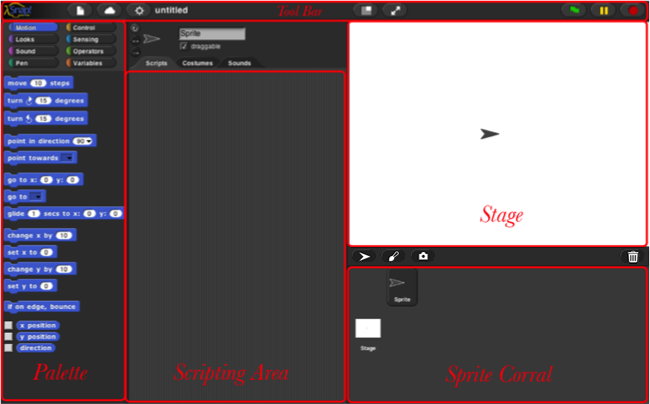
\includegraphics[width=4.32639in,height=2.68958in]{media/image5.png}Start
Snap\emph{!}\textsc{.} You should see the following arrangement of
regions in the window:

(The proportions of these areas may be different, depending on the size
and shape of your browser window.)

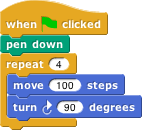
\includegraphics[width=1.47917in,height=1.35417in]{media/image6.png}A
Snap\emph{!} program consists of one or more \emph{scripts,} each of
which is made of \emph{blocks.} Here's a typical script:


\includegraphics[width=2.24653in,height=1.46944in]{media/image7.png}
\includegraphics[width=2.20833in,height=1.13889in]{media/image8.png}The
five blocks that make up this script have three different colors,
corresponding to three of the eight \emph{palettes} in which blocks can
be found. The palette area at the left edge of the window shows one
palette at a time, chosen with the eight buttons just above the palette
area. In this script, the gold blocks are from the Control palette; the
green block is from the Pen palette; and the blue blocks are from the
Motion palette. A script is assembled by dragging blocks from a palette
into the \emph{scripting area} in the middle part of the window. Blocks
snap together (hence the name Snap\emph{!} for the language) when you
drag a block so that its indentation is near the tab of the one above
it:

The white horizontal line is a signal that if you let go of the green
block it will snap into the tab of the gold one.

\subsubsection*{Hat Blocks and Command
Blocks}\label{hat-blocks-and-command-blocks}
\addcontentsline{toc}{subsubsection}{Hat Blocks and Command Blocks}

At the top of the script is a \emph{hat} block, which indicates when the
script should be carried out. Hat block names typically start with the
word ``when''; in the square-drawing example on page 5, the script
should be run when the green flag near the right end of the Snap\emph{!}
tool bar is clicked. (The Snap\emph{!} tool bar is part of the
Snap\emph{!} window, not the same as the browser's or operating system's
menu bar.) A script isn't required to have a hat block, but if not, then
the script will be run only if the user clicks on the script itself. A
script can't have more than one hat block, and the hat block can be used
only at the top of the script; its distinctive shape is meant to remind
you of that.\footnote{One of the hat blocks, the generic ``when
  anything'' block , is subtly different from the others. When the stop
  sign is clicked, or when a project or sprite is loaded, this block
  doesn't test whether the condition in its hexagonal input slot is
  true, so the script beneath it will not run, until some \emph{other}
  script in the project runs (because, for example, you click the green
  flag). When generic when blocks are disabled, the stop sign will be
  square instead of octagonal.}\phantomsection\label{generic_when}{}


\includegraphics[width=1.16667in,height=0.25in]{media/image9.png}The
other blocks in our example script are \emph{command} blocks. Each
command block corresponds to an action that Snap\emph{!} already knows
how to carry out. For example, the block tells the sprite (the arrowhead
shape on the \emph{stage} at the right end of the window) to move ten
steps (a step is a very small unit of distance) in the direction in
which the arrowhead is pointing. We'll see shortly that there can be
more than one sprite, and that each sprite has its own scripts. Also, a
sprite doesn't have to look like an arrowhead, but can have any picture
as a \emph{costume.} The shape of the move block is meant to remind you
of a Lego™ brick; a script is a stack of blocks. (The word ``block''
denotes both the graphical shape on the screen and the procedure, the
action, that the block carries out.)


\includegraphics[width=1.09722in,height=0.35417in]{media/image10.png}The
number 10 in the move block above is called an \emph{input} to the
block. By clicking on the white oval, you can type any number in place
of the 10. The sample script on the previous page uses 100 as the input
value. We'll see later that inputs can have non-oval shapes that accept
values other than numbers. We'll also see that you can compute input
values, instead of typing a particular value into the oval. A block can
have more than one input slot. For example, the glide block located
about halfway down the Motion palette has three inputs.

Most command blocks have that brick shape, but some, like the repeat
block in the sample script, are \emph{C‑shaped.} Most C-shaped blocks
are found in the Control palette. The slot inside the C shape is a
special kind of input slot that accepts a \emph{script} as the input.

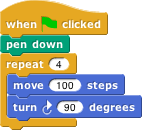
\includegraphics[width=1.47917in,height=1.35417in]{media/image6.png}

the repeat block has two inputs: the number~4 and the script


\includegraphics[width=1.40625in,height=0.48958in]{media/image11.png}In
the sample script

C-shaped blocks can be put in a script in two ways. If you see a white
line and let go, the block will be inserted into the script like any
command block:

But if you see an orange halo and let go, the block will \emph{wrap}
around the haloed blocks:

The halo will always extend from the cursor position to the bottom of
the script:

If you want only some of those blocks, after wrapping you can grab the
first block you don't want wrapped, pull it down, and snap it under the
C-shaped block.

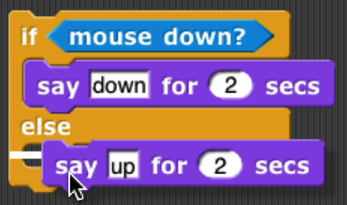
\includegraphics[width=2.31111in,height=1.36667in]{media/image24.png}For
``E-shaped'' blocks with more than one C-shaped slot, only the first
slot will wrap around existing blocks in a script, and only if that
C-shaped slot is empty before wrapping. (You can fill the other slots by
dragging blocks into the desired slot.)

\subsection[\hl{\hfill\break
}Sprites and Parallelism]{\texorpdfstring{\hl{\hfill\break
}\protect
\includegraphics[width=0.34028in,height=0.24306in]{media/image25.png}Sprites
and
Parallelism}{ Sprites and Parallelism}}\label{sprites-and-parallelism}

Just below the stage is the ``new sprite'' button . Click the button to
add a new sprite to the stage. The new sprite will appear in a random
position on the stage, with a random color, but always facing to the
right.

Each sprite has its own scripts. To see the scripts for a particular
sprite in the scripting area, click on the picture of that sprite in the
\emph{sprite corral} in the bottom right corner of the window. Try
putting one of the following scripts in each sprite's scripting area:

\begin{quote}
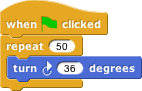
\includegraphics[width=1.55069in,height=0.99375in]{media/image26.png}
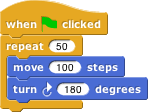
\includegraphics[width=1.54167in,height=1.16667in]{media/image27.png}
\end{quote}

When you click the green flag, you should see one sprite rotate while
the other moves back and forth. This experiment illustrates the way
different scripts can run in parallel. The turning and the moving happen
together. Parallelism can be seen with multiple scripts of a single
sprite also. Try this example:

\begin{quote}
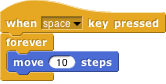
\includegraphics[width=1.72917in,height=0.875in]{media/image28.png}
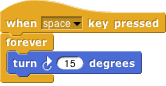
\includegraphics[width=1.72917in,height=0.89583in]{media/image29.png}
\end{quote}

When you press the space key, the sprite should move forever in a
circle, because the move and turn blocks are run in parallel. (To stop
the program, click the red stop sign at the right end of the tool bar.)

\subsubsection{Costumes and Sounds}\label{costumes-and-sounds}


\includegraphics[width=0.31944in,height=0.21528in]{media/image30.png}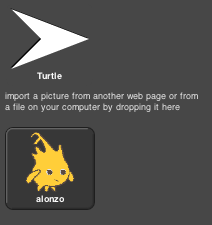
\includegraphics[width=1.76667in,height=1.875in]{media/image31.png}
\includegraphics[width=0.29167in,height=0.16667in]{media/image32.png}To
change the appearance of a sprite, paint or import a new \emph{costume}
for it. To paint a costume, click on the Costumes tab above the
scripting area, and click the paint button . The \emph{Paint Editor}
that appears is explained on page \hyperref[the-paint-editor]{128}.
There are three ways to import a costume. First select the desired
sprite in the sprite corral. Then, one way is to click on the file icon
in the tool bar , then choose the ``Costumes\ldots''menu item. You will
see a list of costumes from the public media library, and can choose
one. The second way, for a costume stored on your own computer, is to
click on the file icon and choose the ``Import\ldots'' menu item. You
can then select a file in any picture format (PNG, JPEG, etc.) supported
by your browser. The third way is quicker if the file you want is
visible on the desktop: Just drag the file onto the Snap\emph{!} window.
In any of these cases, the scripting area will be replaced by something
like this:

Just above this part of the window is a set of three tabs: Scripts,
Costumes, and Sounds. You'll see that the Costumes tab is now selected.
In this view, the sprite's \emph{wardrobe,} you can choose whether the
sprite should wear its Turtle costume or its Alonzo costume. (Alonzo,
the Snap\emph{!} mascot, is named after Alonzo Church, a mathematician
who invented the idea of procedures as data, the most important way in
which Snap\emph{!} is different from Scratch.) You can give a sprite as
many costumes as you like, and then choose which it will wear either by
clicking in its wardrobe or by using the or block in a script. (Every
costume has a number as well as a name. The next costume block selects
the next costume by number; after the highest-numbered costume it
switches to costume 1. The Turtle, costume 0, is never chosen by next
costume.) The Turtle costume is the only one that changes color to match
a change in the sprite's pen color. Protip: switches to the
\emph{previous} costume, wrapping like next costume.


\includegraphics[width=1.80556in,height=0.27778in]{media/image33.png}
\includegraphics[width=1.89583in,height=0.26042in]{media/image38.png}
\includegraphics[width=1.23958in,height=0.26042in]{media/image39.png}In
addition to its costumes, a sprite can have \emph{sounds;} the
equivalent for sounds of the sprite's wardrobe is called its
\emph{jukebox.} Sound files can be imported in any format (WAV, OGG,
MP3, etc.) supported by your browser. Two blocks accomplish the task of
playing sounds. If you would like a script to continue running while the
sound is playing, use the block . In contrast, you can use the block to
wait for the sound\textquotesingle s completion before continuing the
rest of the script\emph{.}

\subsubsection{Inter-Sprite Communication with
Broadcast}\label{inter-sprite-communication-with-broadcast}

Earlier we saw an example of two sprites moving at the same time. In a
more interesting program, though, the sprites on stage will
\emph{interact} to tell a story, play a game, etc. Often one sprite will
have to tell another sprite to run a script. Here's a simple example:


\includegraphics[width=1.71875in,height=0.24939in]{media/image40.png}
\includegraphics[width=0.56944in,height=1.11111in]{media/image41.png}
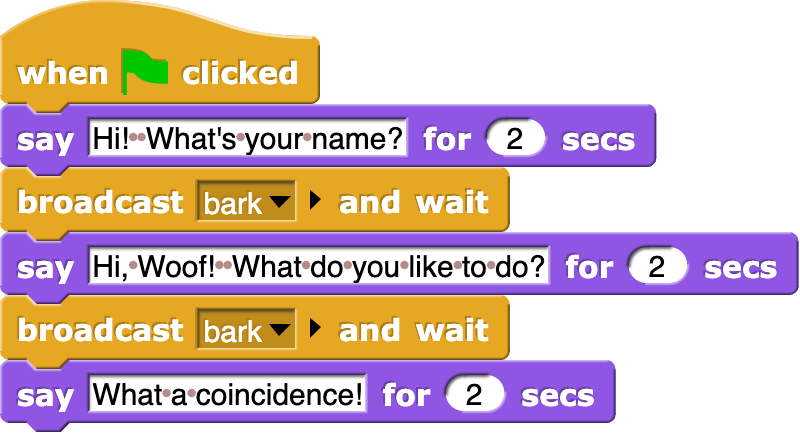
\includegraphics[width=2.78418in,height=1.51042in]{media/image42.png}

\includegraphics[width=1.24306in,height=0.86111in]{media/image43.png}
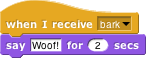
\includegraphics[width=1.52083in,height=0.60417in]{media/image44.png}


\includegraphics[width=1.78958in,height=0.2in]{media/image45.png}
\includegraphics[width=1.8in,height=0.19167in]{media/image46.png}In
the block, the word ``bark'' is just an arbitrary name I made up. When
you click on the downward arrowhead in that input slot, one of the
choices (the only choice, the first time) is ``new,'' which then prompts
you to enter a name for the new broadcast. When this block is run, the
chosen message is sent to \emph{every} sprite, which is why the block is
called ``broadcast.'' (But if you click the right arrow after the
message name, the block becomes , and you can change it to ~to send the
message just to one sprite.) In this program, though, only one sprite
has a script to run when that broadcast is sent, namely the dog. Because
the boy's script uses broadcast and wait rather than just broadcast, the
boy doesn't go on to his next say block until the dog's script finishes.
That's why the two sprites take turns talking, instead of both talking
at once. In Chapter VII, ``Object-Oriented Programming with Sprites,''
you'll see a more flexible way to send a message to a specific sprite
using the tell and ask blocks.

Notice, by the way, that the say block's first input slot is rectangular
rather than oval. This means the input can be any text string, not only
a number. In text input slots, a space character is shown as a brown
dot, so that you can count the number of spaces between words, and in
particular you can tell the difference between an empty slot and one
containing spaces. The brown dots are \emph{not} shown on the stage if
the text is displayed.

The stage has its own scripting area. It can be selected by clicking on
the Stage icon at the left of the sprite corral. Unlike a sprite,
though, the stage can't move. Instead of costumes, it has
\emph{backgrounds:} pictures that fill the entire stage area. The
sprites appear in front of the current background. In a complicated
project, it's often convenient to use a script in the stage's scripting
area as the overall director of the action.

\subsection{Nesting Sprites: Anchors and
Parts}\label{nesting-sprites-anchors-and-parts}

Sometimes it's desirable to make a sort of ``super-sprite'' composed of
pieces that can move together but can also be separately articulated.
The classic example is a person's body made up of a torso, limbs, and a
head. Snap\emph{!} allows one sprite to be designated as the
\emph{anchor} of the combined shape, with other sprites as its
\emph{parts.} To set up sprite nesting, drag the sprite corral icon of a
\emph{part} sprite onto the stage display (not the sprite corral icon!)
of the desired \emph{anchor} sprite. The precise place where you let go
of the mouse button will be the attachment point of the part on the
anchor.

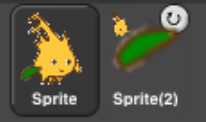
\includegraphics[width=1.63056in,height=0.96528in]{media/image47.png}Sprite
nesting is shown in the sprite corral icons of both anchors and parts:

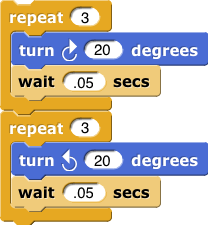
\includegraphics[width=1.44444in,height=1.5625in]{media/image56.png}In
this illustration, it is desired to animate Alonzo's arm. (The arm has
been colored green in this picture to make the relationship of the two
sprites clearer, but in a real project they'd be the same color,
probably.) Sprite, representing Alonzo's body, is the anchor; Sprite(2)
is the arm. The icon for the anchor shows small images of up to three
attached parts at the bottom. The icon for each part shows a small image
of the anchor in its top left corner, and a \emph{synchronous/dangling
rotation flag} in the top right corner. In its initial, synchronous
setting, as shown above, it means that the when the anchor sprite
rotates, the part sprite also rotates as well as revolving around the
anchor. When clicked, it changes from a circular arrow to a straight
arrow, and indicates that when the anchor sprite rotates, the part
sprite revolves around it, but does not rotate, keeping its original
orientation. (The part can also be rotated separately, using its turn
blocks.) Any change in the position or size of the anchor is always
extended to its parts. Also, cloning the anchor (see Section VII. B)
will also clone all its parts.

\emph{Top: turning the part: the green arm. Bottom: turning the anchor,
with the arm synchronous (left) and dangling (right).}

\subsection{Reporter Blocks and
Expressions}\label{reporter-blocks-and-expressions}


\includegraphics[width=1.47in,height=0.52in]{media/image65.png}
\includegraphics[width=0.72917in,height=0.15625in]{media/image66.png}So
far, we've used two kinds of blocks: hat blocks and command blocks.
Another kind is the \emph{reporter} block, which has an oval shape: .
It's called a ``reporter'' because when it's run, instead of carrying
out an action, it reports a value that can be used as an input to
another block. If you drag a reporter into the scripting area by itself
and click on it, the value it reports will appear in a speech balloon
next to the block:

When you drag a reporter block over another block's input slot, a white
``halo'' appears around that input slot, analogous to the white line
that appears when snapping command blocks together:

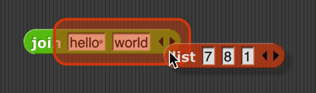
\includegraphics[width=2.11111in,height=0.61806in]{media/image71.png}Don't
drop the input over a \emph{red} halo:

That's used for a purpose explained on page
\hyperref[recursive-calls-to-multiple-input-blocks]{68}.

Here's a simple script that uses a reporter block:

Here the x position reporter provides the first input to the say block.
(The sprite's X position is its horizontal position, how far left
(negative values) or right (positive values) it is compared to the
center of the stage. Similarly, the Y position is measured vertically,
in steps above (positive) or below (negative) the center.)

You can do arithmetic using reporters in the Operators palette:

The round block rounds 35.3905\ldots{} to 35, and the + block adds 100
to that. (By the way, the round block is in the Operators palette, just
like +, but in this script it's a lighter color with black lettering
because Snap\emph{!} alternates light and dark versions of the palette
colors when a block is nested inside another block from the same
palette:

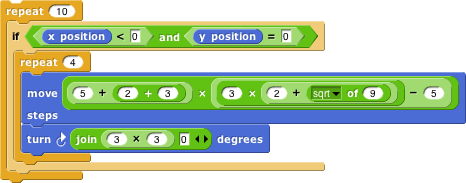
\includegraphics[width=4.85417in,height=1.90625in]{media/image80.png}


\includegraphics[width=1.91667in,height=0.23958in]{media/image81.png}This
aid to readability is called \emph{zebra coloring.}) A reporter block
with its inputs, maybe including other reporter blocks, such as , is
called an \emph{expression.}

\subsection{\texorpdfstring{\hfill\break
Predicates and Conditional
Evaluation}{ Predicates and Conditional Evaluation}}\label{predicates-and-conditional-evaluation}


\includegraphics[width=0.66667in,height=0.1875in]{media/image82.png}
\includegraphics[width=1.20833in,height=0.1875in]{media/image83.png}Most
reporters report either a number, like , or a text string, like . A
\emph{predicate} is a special kind of reporter that always reports true
or false. Predicates have a hexagonal shape:


\includegraphics[width=1.94792in,height=0.26042in]{media/image84.png}
\includegraphics[width=1.07292in,height=0.15625in]{media/image85.png}The
special shape is a reminder that predicates don't generally make sense
in an input slot of blocks that are expecting a number or text. You
wouldn't say , although (as you can see from the picture) Snap\emph{!}
lets you do it if you really want. Instead, you normally use predicates
in special hexagonal input slots like this one:


\includegraphics[width=0.66667in,height=0.56944in]{media/image86.png}The
C-shaped if block runs its input script if (and only if) the expression
in its hexagonal input reports true.

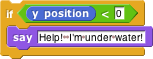
\includegraphics[width=1.59375in,height=0.61458in]{media/image87.png}A
really useful block in animations runs its input script
\emph{repeatedly} until a predicate is satisfied:

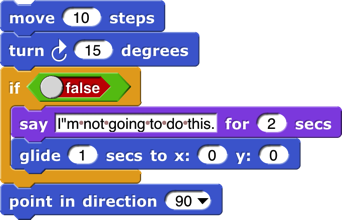
\includegraphics[width=2.28194in,height=1.46875in]{media/image88.png}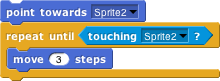
\includegraphics[width=2.29167in,height=0.84375in]{media/image89.png}If,
while working on a project, you want to omit temporarily some commands
in a script, but you don't want to forget where they belong, you can say

Sometimes you want to take the same action whether some condition is
true or false, but with a different input value. For this purpose you
can use the \emph{reporter} if block:


\includegraphics[width=4.20833in,height=0.38542in]{media/image90.png}The
technical term for a true or false value is a ``Boolean'' value; it has
a capital B because it's named after a person, George Boole, who
developed the mathematical theory of Boolean values. Don't get confused;
a hexagonal block is a \emph{predicate,} but the value it reports is a
\emph{Boolean.}

Another quibble about vocabulary: Many programming languages reserve the
name ``procedure'' for Commands (that carry out an action) and use the
name ``function'' for Reporters and Predicates. In this manual, a
\emph{procedure} is any computational capability, including those that
report values and those that don't. Commands, Reporters, and Predicates
are all procedures. The words ``a Procedure type'' are shorthand for
``Command type, Reporter type, or Predicate type.''


\includegraphics[width=1.375in,height=0.24306in]{media/image91.png}
\includegraphics[width=1.375in,height=0.24306in]{media/image92.png}If
you want to put a \emph{constant} Boolean value in a hexagonal slot
instead of a predicate-based expression, hover the mouse over the block
and click on the control that appears:

\subsection{Variables}\label{variables}

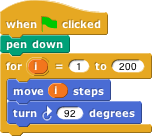
\includegraphics[width=1.58333in,height=1.41667in]{media/image93.png}Try
this script:

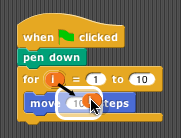
\includegraphics[width=1.88542in,height=1.4375in]{media/image94.png}The
input to the move block is an orange oval. To get it there, drag the
orange oval that's part of the for block:

The orange oval is a \emph{variable:} a symbol that represents a value.
(I took this screenshot before changing the second number input to the
for block from the default 10 to 200, and before dragging in a turn
block.) For runs its script input repeatedly, just like repeat, but
before each repetition it sets the variable i to a number starting with
its first numeric input, adding 1 for each repetition, until it reaches
the second numeric input. In this case, there will be 200 repetitions,
first with i=1, then with i=2, then 3, and so on until i=200 for the
final repetition. The result is that each move draws a longer and longer
line segment, and that's why the picture you see is a kind of spiral.
(If you try again with a turn of 90 degrees instead of 92, you'll see
why this picture is called a ``squiral.'')

\includegraphics[width=3.1875in,height=1.5in]{media/image95.png}The
variable i is created by the for block, and it can only be used in the
script inside the block's C-slot. (By the way, if you don't like the
name i, you can change it by clicking on the orange oval without
dragging it, which will pop up a dialog window in which you can enter a
different name:

``I'' isn't a very descriptive name; you might prefer ``length'' to
indicate its purpose in the script. ``I'' is traditional because
mathematicians tend to use letters between i and n to represent integer
values, but in programming languages we don't have to restrict ourselves
to single-letter variable names.)

\subsubsection{\texorpdfstring{\hfill\break
Global Variables}{ Global Variables}}\label{global-variables}

You can create variables ``by hand'' that aren't limited to being used
within a single block. At the top of the Variables palette, click the
``Make a variable'' button:

\includegraphics[width=3.1875in,height=1.84375in]{media/image96.png}\includegraphics[width=2.05208in,height=2.27083in]{media/image97.png}This
will bring up a dialog window in which you can give your variable a
name:

The dialog also gives you a choice to make the variable available to all
sprites (which is almost always what you want) or to make it visible
only in the current sprite. You'd do that if you're going to give
several sprites individual variables \emph{with the same name,} so that
you can share a script between sprites (by dragging it from the current
sprite's scripting area to the picture of another sprite in the sprite
corral), and the different sprites will do slightly different things
when running that script because each has a different value for that
variable name.

\includegraphics[width=1.65833in,height=2.29167in]{media/image98.png}If
you give your variable the name ``name'' then the Variables palette will
look like this:

\includegraphics[width=1.04167in,height=0.40625in]{media/image99.png}There's
now a ``Delete a variable'' button, and there's an orange oval with the
variable name in it, just like the orange oval in the for block. You can
drag the variable into any script in the scripting area. Next to the
oval is a checkbox, initially checked. When it's checked, you'll also
see a \emph{variable watcher} on the stage:

When you give the variable a value, the orange box in its watcher will
display the value.

\includegraphics[width=1.92708in,height=0.47917in]{media/image100.png}How
\emph{do} you give it a value? You use the set block:

Note that you \emph{don't} drag the variable's oval into the set block!
You click on the downarrow in the first input slot, and you get a menu
of all the available variable names.

If you do choose ``For this sprite only'' when creating a variable, its
block in the palette looks like this:

\includegraphics[width=0.65833in,height=0.14167in]{media/image101.png}
The \emph{location}-pin icon is a bit of a pun on a sprite-\emph{local}
variable. It's shown only in the palette.

\subsubsection{Script Variables}\label{script-variables}

In the name example above, our project is going to carry on an
interaction with the user, and we want to remember their name throughout
the project. That's a good example of a situation in which a
\emph{global} variable (the kind you make with the ``Make a variable''
button) is appropriate. Another common example is a variable called
``score'' in a game project. But sometimes you only need a variable
temporarily, during the running of a particular script. In that case you
can use the script variables block to make the variable:

As in the for block, you can click on an orange oval in the script
variables block without dragging to change its name. You can also make
more than one temporary variable by clicking on the right arrow at the
end of the block to add another variable oval:

\subsubsection[Renaming
variables]{\texorpdfstring{\protect\includegraphics[width=2.08333in,height=0.30208in]{media/image106.png}Renaming
variables}{Renaming variables}}\label{renaming-variables}

There are several reasons why you might want to change the name of a
variable:

\begin{enumerate}
\def\labelenumi{\arabic{enumi}.}
\item
  It has a default name, such as the ``a'' in script variables or the
  ``i'' in for.
\item
  It conflicts with another name, such as a global variable, that you
  want to use in the same script.
\item
  You just decide a different name would be more self-documenting.
\end{enumerate}

In the first and third case, you probably want to change the name
everywhere it appears in that script, or even in all scripts. In the
second case, if you've already used both variables in the script before
realizing that they have the same name, you'll want to look at each
instance separately to decide which ones to rename. Both of these
operations are possible by right-clicking or control-clicking on a
variable oval.

\includegraphics[width=1.61389in,height=1.50764in]{media/image107.png}\includegraphics[width=2.82639in,height=1.25694in]{media/image108.png}\includegraphics[width=1.38194in,height=0.74306in]{media/image109.png}If
you right-click on an orange oval in a context in which the variable is
\emph{used,} then you are able to rename just that one orange oval:

\includegraphics[width=1.70833in,height=0.83333in]{media/image110.png}\includegraphics[width=1.49306in,height=0.74306in]{media/image111.png}If
you right-click on the place where the variable is \emph{defined} (a
script variables block, the orange oval for a global variable in the
Variables palette, or an orange oval that's built into a block such as
the ``i'' in for), then you are given two renaming options, ``rename''
and ``rename all.'' If you choose ``rename,'' then the name is changed
only in that one orange oval, as in the previous case:

\includegraphics[width=1.49306in,height=0.74306in]{media/image112.png}\includegraphics[width=1.70833in,height=0.83333in]{media/image113.png}But
if you choose ``rename all,'' then the name will be changed throughout
the scope of the variable (the script for a script variable, or
everywhere for a global variable):

\subsubsection{Transient variables}\label{transient-variables}

\includegraphics[width=1.29167in,height=1.05556in]{media/image114.png}So
far we've talked about variables with numeric values, or with short text
strings such as someone's name. But there's no limit to the amount of
information you can put in a variable; in Chapter IV you'll see how to
use \emph{lists} to collect many values in one data structure, and in
Chapter VIII you'll see how to read information from web sites. When you
use these capabilities, your project may take up a lot of memory in the
computer. If you get close to the amount of memory available to
Snap\emph{!}, then it may become impossible to save your project. (Extra
space is needed temporarily to convert from Snap\emph{!} 's internal
representation to the form in which projects are exported or saved.) If
your program reads a lot of data from the outside world that will still
be available when you use it next, you might want to have values
containing a lot of data removed from memory before saving the project.
To do this, right-click or control-click on the orange oval in the
Variables palette, to see this menu:

You already know about the rename options, and help\ldots{} displays a
help screen about variables in general. Here we're interested in the
check box next to transient. If you check it, this variable's value will
not be saved when you save your project. Of course, you'll have to
ensure that when your project is loaded, it recreates the needed value
and sets the variable to it.

\subsection{Debugging}\label{debugging}

Snap\emph{!} provides several tools to help you debug a program. They
center around the idea of \emph{pausing} the running of a script partway
through, so that you can examine the values of variables.

\subsubsection{The pause button}\label{the-pause-button}

\includegraphics[width=0.29167in,height=0.16667in]{media/image115.png}\includegraphics[width=0.29167in,height=0.16667in]{media/image116.png}The
simplest way to pause a program is manually, by clicking the pause
button in the top right corner of the window. While the program is
paused, you can run other scripts by clicking on them, show variables on
stage with the checkbox next to the variable in the Variables palette or
with the show variable block, and do all the other things you can
generally do, including modifying the paused scripts by adding or
removing blocks. The button changes shape to and clicking it again
resumes the paused scripts.

\subsubsection{Breakpoints: the pause all
block}\label{breakpoints-the-pause-all-block}

\phantomsection\label{pause_all}{}\includegraphics[width=0.81944in,height=0.21528in]{media/image117.png}The
pause button is great if your program seems to be in an infinite loop,
but more often you'll want to set a \emph{breakpoint,} a particular
point in a script at which you want to pause. The block, near the bottom
of the Control palette, can be inserted in a script to pause when it is
run. So, for example, if your program is getting an error message in a
particular block, you could use pause all just before that block to look
at the values of variables just before the error happens.

\includegraphics[width=1.88333in,height=0.91111in]{media/image118.png}The
pause all block turns bright cyan while paused. Also, during the pause,
you can right-click on a running script and the menu that appears will
give you the option to show watchers for temporary variables of the
script:

But what if the block with the error is run many times in a loop, and it
only errors when a particular condition is true---say, the value of some
variable is negative, which shouldn't ever happen. In the iteration
library (see page \hyperref[libraries-1]{25} for more about how to use
libraries) is a breakpoint block that lets you set a \emph{conditional}
breakpoint, and automatically display the relevant variables before
pausing. Here's a sample use of it:

\includegraphics[width=1.19444in,height=1.33333in]{media/image119.png}(In
this contrived example, variable zot comes from outside the script but
is relevant to its behavior.) When you continue (with the pause button),
the temporary variable watchers are removed by this breakpoint block
before resuming the script. The breakpoint block isn't magic; you could
alternatively just put a pause all inside an if.\footnote{The hide
  variable and show variable blocks can also be used to hide and show
  primitives in the palette. The pulldown menu doesn't include primitive
  blocks, but there's a generally useful technique to give a block input
  values it wasn't expecting using run or
  call:\includegraphics[width=3.9375in,height=0.38889in]{media/image120.png}

  In order to use a block as an input this way, you must explicitly put
  a ring around it, by right-clicking on it and choosing ringify. More
  about rings in Chapter VI.}

\subsubsection{Visible stepping}\label{visible-stepping}

\includegraphics[width=0.29167in,height=0.16667in]{media/image121.png}\includegraphics[width=0.54563in,height=0.15278in]{media/image122.png}\includegraphics[width=0.29167in,height=0.16667in]{media/image123.png}Sometimes
you're not exactly sure where the error is, or you don't understand how
the program got there. To understand better, you'd like to watch the
program as it runs, at human speed rather than at computer speed. You
can do this by clicking the \emph{visible stepping button} ( ), before
running a script or while the script is paused. The button will light up
( ) and a speed control slider will appear in the toolbar. When you
start or continue the script, its blocks and input slots will light up
cyan one at a time:

In this simple example, the inputs to the blocks are constant values,
but if an input were a more complicated expression involving several
reporter blocks, each of those would light up as they are called. Note
that the input to a block is evaluated before the block itself is
called, so, for example, the 100 lights up before the move.

\textbf{. . .}

\includegraphics[width=0.29167in,height=0.16667in]{media/image134.png}The
speed of stepping is controlled by the slider. If you move the slider
all the way to the left, the speed is zero, the pause button turns into
a step button , and the script takes a single step each time you push
it. The name for this is \emph{single stepping.}

If several scripts that are visible in the scripting area are running at
the same time, all of them are stepped in parallel. However, consider
the case of two repeat loops with different numbers of blocks. While not
stepping, each script goes through a complete cycle of its loop in each
display cycle, despite the difference in the length of a cycle. In order
to ensure that the visible result of a program on the stage is the same
when stepped as when not stepped, the shorter script will wait at the
bottom of its loop for the longer script to catch up.

When we talk about custom blocks in Chapter III, we'll have more to say
about visible stepping as it affects those blocks.

\subsection{Etcetera}\label{etcetera}

This manual doesn't explain every block in detail. There are many more
motion blocks, sound blocks, costume and graphics effects blocks, and so
on. You can learn what they all do by experimentation, and also by
reading the ``help screens'' that you can get by right-clicking or
control-clicking a block and selecting ``help\ldots'' from the menu that
appears. If you forget what palette (color) a block is, but you remember
at least part of its name, type control-F and enter the name in the text
block that appears in the palette area.

Here are the primitive blocks that don't exist in Scratch:

\includegraphics[width=1.25in,height=0.22917in]{media/image135.png}\includegraphics[width=1.05208in,height=0.22917in]{media/image136.png}
reports a new costume consisting of everything that's drawn on the stage
by any sprite. Right-clicking the block in the scripting area gives the
option to change it to if vector logging is enabled. See page
\hyperref[logpenvectors]{116}.

\includegraphics[width=2.08333in,height=0.375in]{media/image137.png}Print
characters in the given point size on the stage, at the sprite's
position and in its direction. The sprite moves to the end of the text.
(That's not always what you want, but you can save the sprite's position
before using it, and sometimes you need to know how big the text turned
out to be, in turtle steps.) If the pen is down, the text will be
underlined.

\includegraphics[width=1.20069in,height=0.51389in]{media/image138.png}Takes
a sprite as input. Like stamp except that the costume is stamped onto
the selected sprite instead of onto the stage. (Does nothing if the
current sprite doesn't overlap the chosen sprite.)

\includegraphics[width=1.19167in,height=0.33889in]{media/image139.png}Takes
a sprite as input. Erases from that sprite's costume the area that
overlaps with the current sprite's costume. (Does not affect the costume
in the chosen sprite's wardrobe, only the copy currently visible.)

Runs only this script

until finished. In the Control palette even though it's gray.

\includegraphics[width=0.52986in,height=0.5in]{media/image140.png}\includegraphics[width=0.98958in,height=0.25972in]{media/image141.png}\includegraphics[width=1.32986in,height=0.42986in]{media/image142.png}
See page \hyperref[generic_when]{6}. See page \hyperref[pause_all]{17}.

\includegraphics[width=1.71in,height=0.23in]{media/image143.png}Reporter
version of the if/else primitive command block. Only one of the two
branches is evaluated, depending on the value of the first input.

\includegraphics[width=1.83in,height=0.61in]{media/image144.png}Looping
block like repeat but with an index variable.

\includegraphics[width=1.37986in,height=0.28958in]{media/image145.png}Declare
local variables in a script.

\includegraphics[width=0.86in,height=0.19in]{media/image146.png}\includegraphics[width=0.72in,height=0.2in]{media/image147.png}\includegraphics[width=1.17in,height=0.18in]{media/image148.png}
See page \hyperref[url]{91}.

reports the value of a graphics effect.

Constant true or false value. See page
\hyperref[predicates-and-conditional-evaluation]{12}.

\includegraphics[width=2.13in,height=0.18in]{media/image153.png} Create
a primitive using JavaScript. (This block is disabled by default; the
user must check ``Javascript extensions'' in the setting menu \emph{each
time} a project is loaded.)

The at block lets you examine the screen pixel directly behind the
rotation center of a sprite, the mouse, or an arbitrary (x,y) coordinate
pair dropped onto the second menu slot. The first five items of the left
menu let you examine the color visible at the position. (The ``RGBA''
option reports a list.) The ``sprites'' option reports a list of all
sprites, including this one, any point of which overlaps this sprite's
rotation center (behind or in front). This is a hyperblock with respect
to its second input.

\includegraphics[width=2.44583in,height=1.32639in]{media/image162.png}\includegraphics[width=2.35556in,height=0.38889in]{media/image163.png}
Checks the data type of a value.

\textbf{Blocks only for the Stage:}

Get or set selected global flags.

Turn the text into a list, using the second input as the delimiter
between items. The default delimiter, indicated by the brown dot in the
input slot, is a single space character. ``Letter'' puts each character
of the text in its own list item. ``Word'' puts each word in an item.
(Words are separated by any number of consecutive space, tab, carriage
return, or newline characters.) ``Line'' is a newline character (0xa);
``tab'' is a tab character (0x9); ``cr'' is a carriage return (0xd).
``Csv'' and ``json'' split formatted text into lists of lists; see page
\hyperref[comma-separated-values]{54}. ``Blocks'' takes a script as the
first input, reporting a list structure representing the structure of
the script. See Chapter XI.

\includegraphics[width=1.47986in,height=0.18958in]{media/image170.png}For
lists, reports true only if its two input values are the very same list,
so changing an item in one of them is visible in the other. (For =,
lists that look the same are the same.) For text strings, uses
case-sensitive comparison, unlike =, which is case-independent.

These \emph{hidden} blocks can be found with the relabel option of any
dyadic arithmetic block. They're hidden partly because writing them in
Snap\emph{!} is a good, pretty easy programming exercise. Note: the two
inputs to atan2 are Δ\emph{x} and Δ\emph{y} in that order, because we
measure angles clockwise from north. Max and min are \emph{variadic;} by
clicking the arrowhead, you can provide additional inputs.

\includegraphics[width=0.63in,height=0.19in]{media/image177.png}
\includegraphics[width=0.63in,height=0.19in]{media/image178.png}
\includegraphics[width=0.63in,height=0.19in]{media/image179.png}
Similarly, these hidden predicates can be found by relabeling the
relational predicates.

\textbf{Metaprogramming (see Chapter XI.} \textbf{, page
\hyperref[metaprogramming]{101})}

These blocks support \emph{metaprogramming,} which means manipulating
blocks and scripts as data. This is not the same as manipulating
procedures (see Chapter VI. ), which are what the blocks \emph{mean;} in
metaprogramming the actual blocks, what you see on the screen, are the
data. This capability is new in version 8.0.

\textbf{First class list blocks (see Chapter IV, page
\hyperref[first-class-lists]{46}):}

Numbers from will count up or down.

The script input to for each can refer to an

item of the list with the item variable.

\textbf{\hfill\break
}\includegraphics[width=0.83in,height=0.21in]{media/image224.png}
\includegraphics[width=1.43in,height=0.21in]{media/image225.png} report
the sprite or mouse position as a two-item vector (x,y).

\textbf{First class procedure blocks (see Chapter VI, page
\hyperref[procedures-as-data]{65}):}

\textbf{First class continuation blocks (see Chapter X, page
\hyperref[continuations]{93}):}

\textbf{First class sprite, costume, and sound blocks (see Chapter VII,
page \hyperref[object-oriented-programming-with-sprites]{73}):}

Object is a hyperblock.

\textbf{Scenes:}

\includegraphics[width=2.38in,height=1.32in]{media/image280.png}The
major new feature of version 7.0 is \emph{scenes:} A project can include
within it sub-projects, called scenes, each with its own stage, sprites,
scripts, and so on. This block makes another scene active, replacing the
current one.

Nothing is automatically shared between scenes: no sprites, no blocks,
no variables. But the old scene can send a message to the new one, to
start it running, with optional payload as in broadcast (page
\hyperref[broadcast]{23}).

\includegraphics[width=2.54in,height=0.31in]{media/image281.png}In
particular, you can say

\begin{quote}
if the new scene expects to be started with a green flag signal.
\end{quote}

\textbf{\hfill\break
These aren't new blocks but they have a new feature:}

These accept two-item (x,y) lists as input, and have extended menus
(also including other sprites):

``Center'' means the center of the stage, the point at (0,0).
``Direction'' is in the point in direction sense, the direction that
would leave this sprite pointing toward another sprite, the mouse, or
the center. ``Ray length'' is the distance from the center of this
sprite to the nearest point on the other sprite, in the current
direction.

The stop block has two extra menu choices. Stop this block is used
inside the definition of a custom block to stop just this invocation of
this custom block and continue the script that called it. Stop all but
this script is good at the end of a game to stop all the game pieces
from moving around, but keep running this script to provide the user's
final score. The last two menu choices add a tab at the bottom of the
block because the current script can continue after it.

The new ``pen trails'' option is true if the sprite is touching any
drawn or stamped ink on the stage. Also, touching will not detect hidden
sprites, but a hidden sprite can use it to detect visible sprites.

\includegraphics[width=1.05972in,height=0.27986in]{media/image304.png}\includegraphics[width=2.43333in,height=0.3in]{media/image305.png}The
video block has a snap option that takes a snapshot and reports it as a
costume. It is hyperized with
\includegraphics[width=1.05208in,height=0.28125in]{media/image306.png}respect
to its second input.

The ``neg'' option is a monadic negation operator, equivalent to .
``lg'' is log\textsubscript{2}. ``id'' is the identity function, which
reports its input. ``sign'' reports 1 for positive input, 0 for zero
input, or -1 for negative input.

name changed to clarify that it's different from

+ and × are \emph{variadic:} they take two or more inputs. If you drop a
list on the arrowheads, the block name changes to sum or product.

I

Extended mouse interaction events, sensing clicking, dragging, hovering,
etc. The ``stopped'' option triggers when all scripts are stopped, as
with the stop button; it is useful for robots whose hardware interface
must be told to turn off motors. A when I am stopped script can run only
for a limited time.

\phantomsection\label{broadcast}{}Extended broadcast: Click the right
arrowhead to direct the message to a single sprite or the stage. Click
again to add any value as a payload to the message.

Extended when I receive: Click the right arrowhead to expose a script
variable (click on it to change its name, like any script variable) that
will be set to the data of a matching broadcast. If the first input is
set to ``any message,'' then the data variable will be set to the
message, if no payload is included with the broadcast, or to a two-item
list containing the message and the payload.

\includegraphics[width=1.68in,height=0.38in]{media/image355.png} If the
input is set to ``any key,'' then a right arrowhead appears:

\begin{quote}
\includegraphics[width=2.25in,height=0.41944in]{media/image356.png}\includegraphics[width=1.81944in,height=0.37986in]{media/image357.png}and
if you click it, a script variable key is created whose value is the key
that was pressed. (If the key is one that' represented in the input menu
by a word or phrase, e.g., ``enter'' or ``up arrow,'' then the value of
key will be that word or phrase, \emph{except for} the space character,
which is represented as itself in key.)\\
\phantomsection\label{ask_lists}{}
\end{quote}

The RGB(A) option accepts a single number, which is a grayscale value
0-255; a two-number list, grayscale plus opacity 0-255; a three-item RGB
list, or a four-item RGBA list.

These ask features and more in the Menus library.

The of block has an extended menu of attributes of a sprite. Position
reports an (x,y) vector. Size reports the percentage of normal size, as
controlled by the set size block in the Looks category. Left, right,
etc. report the stage coordinates of the corresponding edge of the
sprite's bounding box. Variables reports a list of the names of all
variables in scope (global, sprite-local, and script variables if the
right input is a script.

\subsection{\texorpdfstring{\hfill\break
Libraries}{ Libraries}}\label{libraries}

\phantomsection\label{libraries-1}{}\includegraphics[width=0.31944in,height=0.18056in]{media/image384.png}There
are several collections of useful procedures that aren't Snap\emph{!}
primitives, but are provided as libraries. To include a library in your
project, choose the Libraries\ldots{} option in the file ( ) menu.

The library menu is divided into five broad categories. The first is,
broadly, utilities: blocks that might well be primitives. They might be
useful in all kinds of projects.

The second category is blocks related to media computation: ones that
help in dealing with costumes and sounds (a/k/a Jens libraries). There
is some overlap with ``big data'' libraries, for dealing with large
lists of lists.

The third category is, roughly, specific to non-media applications
(a/k/a Brian libraries). Three of them are imports from other
programming languages: words and sentences from Logo, array functions
from APL, and streams from Scheme. Most of the others are to meet the
needs of the BJC curriculum.

The fourth category is major packages (extensions) provided by users.

The fifth category provides support for hardware devices such as robots,
through general interfaces, replacing specific hardware libraries in
versions before 7.0.

When you click on the one-line description of a library, you are shown
the actual blocks in the library and a longer explanation of its
purpose. You can browse the libraries to find one that will satisfy your
needs.

The libraries and their contents may change, but as of this writing the
list library has these blocks:

\includegraphics[width=1.84861in,height=2.49236in]{media/image387.png}
(The lightning bolt before the name in several of these blocks means
that they use compiled HOFs or JavaScript primitives to achieve optimal
speed. They are officially considered experimental.) Remove duplicates
from reports a list in which no two items are equal. The sort block
takes a list and a two-input comparison predicate, such as \textless,
and reports a list with the items sorted according to that comparison.
The assoc block is for looking up a key in an \emph{association list:} a
list of two-item lists. In each two-item list, the first is a \emph{key}
and the second is a \emph{value.} The inputs are a key and an
association list; the block reports the first key-value pair whose key
is equal to the input key.

For each item is a variant of the primitive version that provides a \#
variable containing the position in the input list of the currently
considered item. Multimap is a version of map that allows multiple list
inputs, in which case the mapping function must take as many inputs as
there are lists; it will be called with all the first items, all the
second items, and so on. Zip takes any number of lists as inputs; it
reports a list of lists: all the first items, all the second items, and
so on. The no-name identity function reports its input.

Sentence and sentence➔list are borrowed from the word and sentence
library (page \hyperref[wordsent]{27}) to serve as a variant of append
that accepts non-lists as inputs. Printable takes a list structure of
any depth as input and reports a compact representation of the list as a
text string.

The iteration, composition library has these blocks:

\includegraphics[width=1.68889in,height=4.75in]{media/image388.png}Catch
and throw provide a nonlocal exit facility. You can drag the tag from a
catch block to a throw inside its C-slot, and the throw will then jump
directly out to the matching catch without doing anything in between.

If do and pause all is for setting a breakpoint while debugging code.
The idea is to put show variable blocks for local variables in the
C-slot; the watchers will be deleted when the user continues from the
pause.

Ignore is used when you need to call a reporter but you don't care about
the value it reports. (For example, you are writing a script to time how
long the reporter takes.)

The cascade blocks take an initial value and call a function repeatedly
on that value, \emph{f}(\emph{f}(\emph{f}(\emph{f}\ldots(\emph{x})))).

The compose block takes two functions and reports the function
\emph{f}(\emph{g}(\emph{x})).

\includegraphics[width=1.04444in,height=0.16111in]{media/image389.png}\includegraphics[width=3.15278in,height=0.29861in]{media/image390.png}The
first three repeat blocks are variants of the primitive repeat until
block, giving all four combinations of whether the first test happens
before or after the first repetition, and whether the condition must be
true or false to continue repeating. The last repeat block is like the
repeat primitive, but makes the number of repetitions so far available
to the repeated script. The next two blocks are variations on for: the
first allows an explicit step instead of using ±1, and the second allows
any values, not just numbers; inside the script you say

\includegraphics[width=3.44097in,height=1.36111in]{media/image391.png}\includegraphics[width=3.70972in,height=1.17153in]{media/image392.png}replacing
the grey block in the picture with an expression to give the next
desired value for the loop index. Pipe allows reordering a nested
composition with a left-to-right one:

The stream library has these blocks:

\includegraphics[width=3.16111in,height=2.15347in]{media/image393.png}\emph{Streams}
are a special kind of list whose items are not computed until they are
needed. This makes certain computations more efficient, and also allows
the creation of lists with infinitely many items, such as a list of all
the positive integers. The first five blocks are stream versions of the
list blocks in front of, item 1 of, all but first of, map, and keep.
Show stream takes a stream and a number as inputs, and reports an
ordinary list of the first \emph{n} items of the stream. Stream is like
the primitive list; it makes a finite stream from explicit items. Sieve
is an example block that takes as input the stream of integers starting
with 2 and reports the stream of all the prime numbers. Stream with
numbers from is like the numbers from block for lists, except that there
is no endpoint; it reports an infinite stream of numbers.

The \phantomsection\label{wordsent}{}word and sentence library has these
blocks:

\includegraphics[width=1.67986in,height=3.64306in]{media/image394.png}This
library has the goal of recreating the Logo approach to handling text: A
text isn't best viewed as a string of characters, but rather as a
\emph{sentence}, made of \emph{words,} each of which is a string of
\emph{letters.} With a few specialized exceptions, this is why people
put text into computers: The text is sentences of natural (i.e., human)
language, and the emphasis is on words as constitutive of sentences. You
barely notice the letters of the words, and you don't notice the spaces
between them at all, unless you're proof-reading. (Even then:
Proofreading is \emph{diffciult,} because you see what you expect to
see, what will make the snetence make sense, rather than the misspelling
in front of of your eyes.) Internally, Logo stores a sentence as a list
of words, and a word as a string of letters.

Inexplicably, the designers of Scratch chose to abandon that tradition,
and to focus on the representation of text as a string of characters.
The one vestige of the Logo tradition from which Scratch developed is
the block named letter (1) of (world), rather than character (1) of
(world). Snap\emph{!} inherits its text handling from Scratch.

In Logo, the visual representation of a sentence (a list of words) looks
like a natural language sentence: a string of words with spaces between
them. In Snap\emph{!}, the visual representation of a list looks nothing
at all like natural language. On the other hand, representing a sentence
as a string means that the program must continually re-parse the text on
every operation, looking for spaces, treating multiple consecutive
spaces as one, and so on. Also, it's more convenient to treat a sentence
as a list of words rather than a string of words because in the former
case you can use the higher order functions map, keep, and combine on
them. This library attempts to be agnostic as to the internal
representation of sentences. The sentence selectors accept any
combination of lists and strings; there are two sentence constructors,
one to make a string (join words) and one to make a list (sentence).

The selector names come from Logo, and should be self-explanatory.
However, because in a block language you don't have to type the block
name, instead of the terse butfirst or the cryptic bf we spell out ``all
but first of'' and include ``word'' or ``sentence'' to indicate the
intended domain. There's no first letter of block because letter 1 of
serves that need. Join words (the sentence-as-string constructor) is
like the primitive join except that it puts a space in the reported
value between each of the inputs. Sentence (the List-colored
sentence-as-list constructor) accepts any number of inputs, which can be
words, sentences-as-lists, or sentences-as-strings. (If inputs are lists
of lists, only one level of flattening is done.) Sentence reports a list
of words; there will be no empty words or words containing spaces. The
four blocks with right-arrows in their names convert back and forth
between text strings (words or sentences) and lists. (Splitting a word
into a list of letters is unusual unless you're a linguist investigating
orthography.) Printable takes a list (including a deep list) of words as
input and reports a text string in which parentheses are used to show
the structure, as in Lisp/Scheme.

The pixels library has one block:

\includegraphics[width=0.77917in,height=0.62986in]{media/image395.png}Costumes
are first class data in Snap\emph{!}. Most of the processing of costume
data is done by primitive blocks in the Looks category. (See page
\hyperref[media-computation-with-costumes]{79}.) This library provides
snap, which takes a picture using your computer's camera and reports it
as a costume.

The bar charts library has these blocks:

\includegraphics[width=3.43056in,height=1.91667in]{media/image396.png}Bar
chart takes a table (typically from a CSV data set) as input and reports
a summary of the table grouped by the field in the specified column
number. The remaining three inputs are used only if the field values are
numbers, in which case they can be grouped into buckets (e.g., decades,
centuries, etc.). Those inputs specify the smallest and largest values
of interest and, most importantly, the width of a bucket (10 for
decades, 100 for centuries). If the field isn\textquotesingle t numeric,
leave these three inputs empty or set them to zero. Each string value of
the field is its own bucket, and they appear sorted alphabetically.

Bar chart reports a new table with three columns. The first column
contains the bucket name or smallest number. The second column contains
a nonnegative integer that says how many records in the input table fall
into this bucket. The third column is a subtable containing the actual
records from the original table that fall into the bucket. Plot bar
chart takes the table reported by bar chart and graphs it on the stage,
with axes labelled appropriately. The remaining blocks are helpers for
those.

If your buckets aren\textquotesingle t of constant width, or you want to
group by some function of more than one field, load the "Frequency
Distribution Analysis" library instead.

The multi-branched conditional library has these blocks:

\includegraphics[width=1.85in,height=2.47986in]{media/image397.png}The
catch and throw blocks duplicate ones in the iteration library, and are
included because they are used to implement the others. The cases block
sets up a multi-branch conditional, similar to cond in Lisp or switch in
C-family languages. The first branch is built into the cases block; it
consists of a Boolean test in the first hexagonal slot and an action
script, in the C-slot, to be run if the test reports true. The remaining
branches go in the variadic hexagonal input at the end; each branch
consists of an else if block, which includes the Boolean test and the
corresponding action script, except possibly for the last branch, which
can use the unconditional else block. As in other languages, once a
branch succeeds, no other branches are tested.

\subsubsection{}\label{section-1}

The variadic library has these blocks:

\includegraphics[width=1.19653in,height=0.41667in]{media/image398.png}These
are versions of the associative operators and, and or that take any
number of inputs instead of exactly two inputs. As with any variadic
input, you can also drop a list of values onto the arrowheads instead of
providing the inputs one at a time As of version 8.0, the arithmetic
operators sum, product, minimum, and maximum are no longer included,
because the primitive operators +. ×, min, and max are themselves
variadic.

The colors and crayons library has these blocks:

It is intended as a more powerful replacement for the primitive set pen
block, including \emph{first class color} support; HSL color
specification as a better alternative to the HSV that Snap\emph{!}
inherits from JavaScript; a ``fair hue'' scale that compensates for the
eye's grouping a wide range of light frequencies as green while
labelling mere slivers as orange or yellow; the X11/W3C standard color
names; RGB in hexadecimal; a linear color scale (as in the old days, but
better) based on fair hues and including shades (darker colors) and
grayscale. Another linear scale is a curated set of 100 ``crayons,''
explained further on the next page.

\includegraphics[width=1.13333in,height=0.23333in]{media/image413.png}\includegraphics[width=0.95in,height=0.225in]{media/image414.png}Colors
are created by the block (for direct user selection), the color from
block to specify a color numerically, or by , which reports the color
currently in use by the pen. The from color block reports names or
numbers associated with a color:

\includegraphics[width=4.83333in,height=0.43056in]{media/image415.png}Colors
can be created from other colors:

The three blocks with pen in their names are improved versions of
primitive Pen blocks. In principle set pen, for example, could be
implemented using a (hypothetical) set pen to color composed with the
color from block, but in fact set pen benefits from knowing how the pen
color was set in its previous invocation, so it's implemented separately
from color from. Details in Appendix A.

\includegraphics[width=7.5in,height=0.25in]{media/image416.png}The
recommended way to choose a color is from one of two linear scales: the
continuous \emph{color numbers} and the discrete \emph{crayons:}

\includegraphics[width=7.5in,height=0.25in]{media/image417.png}

\includegraphics[width=4in,height=0.20833in]{media/image418.png}Color
numbers are based on \emph{fair hues,} a modification of the spectrum
(rainbow) hue scale that devotes less space to green and more to orange
and yellow, as well as promoting brown to a real color. Here is the
normal hue scale, for reference:

\includegraphics[width=4in,height=0.20833in]{media/image419.png}Here is
the fair hue scale:

\includegraphics[width=5in,height=0.20833in]{media/image416.png}Here is
the color number scale:

(The picture is wider so that pure spectral colors line up with the fair
hue scale.)

\includegraphics[width=5in,height=0.20833in]{media/image417.png}And here
are the 100 crayons:

The color from block, for example, provides different pulldown menus
depending on which scale you choose:

\includegraphics[width=2.41667in,height=0.34444in]{media/image420.png}You
can also type the crayon name: There are many scales:

\includegraphics[width=4.29167in,height=1.90972in]{media/image427.png}

The white slot at the end of some of the blocks has two purposes. It can
be used to add a transparency to a color (0=opaque, 100=transparent):

or it can be expanded to enter three or four numbers for a vector
directly into the block, so these are equivalent:

But note that a transparency number in a four-number RGBA vector is on
the scale 255=opaque, 0=transparent, so the following are \emph{not}
equivalent:

Set pen crayon to provides the equivalent of a box of 100 crayons. They
are divided into color groups, so the menu in the set pen crayon to
input slot has submenus. The colors are chosen so that starting
\includegraphics[width=4.36528in,height=0.51528in]{media/image440.png}from
crayon 0, change pen crayon by 10 rotates through an interesting, basic
set of ten colors:

\includegraphics[width=4.35556in,height=0.28194in]{media/image441.png}Using
change pen crayon by 5 instead gives ten more colors, for a total of 20:

(Why didn't we use the colors of the 100-crayon Crayola™ box? A few
reasons, one of which is that some Crayola colors aren't representable
on RGB screens. Some year when you have nothing else to do, look up
``color space'' on Wikipedia. Also ``crayon.'' Oh, it's deliberate that
change pen crayon by 5 doesn't include white, since that's the usual
stage background color. White is crayon 14.) Note that crayon 43 is
``Variables''; all the standard block colors are included.

See Appendix A (page \hyperref[crayons-and-color-numbers]{139}) for more
information.

\includegraphics[width=1.51in,height=0.9in]{media/image442.png}The
\textbf{crayon library} has only the crayon features, without the rest
of the colors package.

The catch errors library has these blocks:

\includegraphics[width=0.43056in,height=0.15278in]{media/image443.png}\includegraphics[width=3.04167in,height=1.39583in]{media/image444.png}The
safely try block allows you to handle errors that happen when your
program is run within the program, instead of stopping the script with a
red halo and an obscure error message. The block runs the script in its
first C-slot. If it finishes without an error, nothing else happens. But
if an error happens, the code in the second C-slot is run. While that
second script is running, the variable contains the text of the error
message that would have been displayed if you weren't catching the
error. The error block is sort of the opposite: it lets your program
\emph{generate} an error message, which will be displayed with a red
halo unless it is caught by safely try. Safely try reporting is the
reporter version of safely try.

The text costumes library has only two blocks:

\includegraphics[width=0.53472in,height=0.20833in]{media/image445.png}\includegraphics[width=1.92in,height=0.45078in]{media/image446.png}Costume
from text reports a costume that can be used with the switch to
\includegraphics[width=3.25972in,height=0.18958in]{media/image447.png}costume
block to make a button:

Costume with background reports a costume made from another costume by
coloring its background, taking a color input like the set pen color to
RGB(A) block and a number of turtle steps of padding around the original
costume. These two blocks work together to make even better buttons:

\includegraphics[width=5.51in,height=0.68in]{media/image448.png}

The text to speech library has these blocks:

\includegraphics[width=2.275in,height=0.8in]{media/image449.png}This
library interfaces with a capability in up-to-date browsers, so it might
not work for you. It works best if the accent matches the text!

The parallelization library contains these blocks:

\includegraphics[width=1.17986in,height=1.25972in]{media/image450.png}The
two do in parallel blocks take any number of scripts as inputs. Those
scripts will be run in parallel, like ordinary independent scripts in
the scripting area. The and wait version waits until all of those
scripts have finished before continuing the script below the block.

\includegraphics[width=1.37778in,height=1.48333in]{media/image451.png}The
create variables library has these blocks:

These blocks allow a program to perform the same operation as the

button, making global, sprite local, or script variables, but allowing
the program to compute the variable name(s). It can also set and find
the values of these variables, show and hide their stage watchers,
delete them, and find out if they already exist.

The getters and setters library has these blocks:

\includegraphics[width=1.875in,height=1.05in]{media/image452.png}\includegraphics[width=0.29167in,height=0.16667in]{media/image453.png}The
purpose of this library is to allow program access to the settings
controlled by user interface elements, such as the settings menu. The
setting block reports a setting; the set flag block sets yes-or-no
options that have checkboxes in the user interface, while the set value
block controls settings with numeric or text values, such as project
name.

Certain settings are ordinarily remembered on a per-user basis, such as
the ``zoom blocks'' value. But when these settings are changed by this
library, the change is in effect only while the project using the
library is loaded. No permanent changes are made. Note: this library has
not been converted for version 7.0, so you'll have to enable Javascript
extensions to use it.

The bignums, rationals, complex \#s library has these blocks:

\includegraphics[width=1.875in,height=1.55in]{media/image454.png}The USE
BIGNUMS block takes a Boolean input, to turn the infinite precision
feature on or off. When on, all of the arithmetic operators are
redefined to accept and report integers of any number of digits (limited
only by the memory of your computer) and, in fact, the entire Scheme
numeric tower, with exact rationals and with complex numbers. The Scheme
number block has a list of functions applicable to Scheme numbers,
including subtype predicates such as rational? and infinite?, and
selectors such as numerator and real-part.

The ! block computes the factorial function, useful to test whether
bignums are turned on. Without bignums:

With bignums:

The 375-digit value of 200! isn't readable on this page, but if you
right-click on the block and choose ``result pic,'' you can open the
resulting picture in a browser window and scroll through it. (These
values end with a bunch of zero digits. That's not roundoff error; the
prime factors of 100! and 200! include many copies of 2 and 5.) The
block with no name is a way to enter things like 3/4 and 4+7i into
numeric input slots by converting the slot to Any type.

The strings, multi-line input library provides these blocks:

\includegraphics[width=3.9375in,height=2.04167in]{media/image463.png}All
of these could be written in Snap\emph{!} itself, but these are
implemented using the corresponding JavaScript library functions
directly, so they run fast. They can be used, for example, in scraping
data from a web site. The command use case-independent comparisons
applies only to this library. The multiline block accepts and reports a
text input that can include newline characters.

The animation library has these blocks:

\includegraphics[width=4.0125in,height=2.33125in]{media/image464.png}Despite
the name, this isn't only about graphics; you can animate the values of
a variable, or anything else that's expressed numerically.

\includegraphics[width=0.96528in,height=0.19444in]{media/image465.png}The
central idea of this library is an \emph{easing function,} a reporter
whose domain and range are real numbers between 0 and 1 inclusive. The
function represents what fraction of the ``distance'' (in quotes because
it might be any numeric value, such as temperature in a simulation of
weather) from here to there should be covered in what fraction of the
time. A linear easing function means steady progression. A quadratic
easing function means starting slowly and accelerating. (Note that,
since it's a requirement that \emph{f}(0)=0 and \emph{f}(1)=1, there is
only one linear easing function, \emph{f}(\emph{x})=\emph{x}, and
similarly for other categories.) The block reports some of the common
easing functions.

\includegraphics[width=4.63194in,height=0.63194in]{media/image466.png}The
two Motion blocks in this library animate a sprite. Glide always
animates the sprite's motion. Animate's first pulldown menu input allows
you to animate horizontal or vertical motion, but will also animate the
sprite's direction or size. The animate block in Control lets you
animate any numeric quantity with any easing function. The getter and
setter inputs are best explained by example:

\includegraphics[width=3.40972in,height=0.25694in]{media/image467.png}is
equivalent to

The other blocks in the library are helpers for these four.

The serial ports library contains these blocks:

\includegraphics[width=1.73264in,height=1.03472in]{media/image468.png}It
is used to allow hardware developers to control devices such as robots
that are

connected to your computer via a serial port.

The frequency distribution analysis library has these blocks:

\includegraphics[width=4.02708in,height=2.39583in]{media/image469.png}

This is a collection of tools for analyzing large data sets and plotting
histograms of how often some value is found in some column of the table
holding the data.

For more information go here:

https://tinyurl.com/jens-data

The audio comp library includes these blocks:

\includegraphics[width=3.54167in,height=2.98125in]{media/image470.png}This
library takes a sound, one that you record or one from our collection of
sounds, and manipulates it by systematically changing the intensity of
the samples in the sound and by changing the sampling rate at which the
sound is reproduced. Many of the blocks are helpers for the plot sound
block, used to plot the waveform of a sound. The play sound (primitive)
block plays a sound. \_\_ Hz for reports a sine wave as a list of
samples.

The web services library has these blocks:

\includegraphics[width=3.40972in,height=1.10417in]{media/image471.png}The
first block is a generalization of the primitive url block, allowing
more control over the various options in web requests: GET, POST, PUT,
and DELETE, and fine control over the content of the message sent to the
server. Current location reports your latitude and longitude. Listify
takes some text in JSON format (see page
\hyperref[multi-dimensional-lists-and-json]{54}) and converts it to a
structured list. Value at key looks up a key-value pair in a (listified)
JSON dictionary. The key:value: block is just a constructor for an
abstract data type used with the other blocks

The database library contains these blocks:

\includegraphics[width=2.26389in,height=1.22222in]{media/image472.png}It
is used to keep data that persist from one Snap\emph{!} session to the
next, if you use the same browser and the same login.

The world map library has these blocks:

\includegraphics[width=2.44236in,height=3.40278in]{media/image473.png}Using
any of the command blocks puts a map on the screen, in a layer in front
of the stage's background but behind the pen trails layer (which is in
turn behind all the sprites). The first block asks your browser for your
current physical location, for which you may be asked to give
permission. The next two blocks get and set the map's zoom amount; the
default zoom of 10 fits from San Francisco not quite down to Palo Alto on
the screen. A zoom of 1 fits almost the entire world. A zoom of 3 fits
the United States; a zoom of 5 fits Germany. The zoom can be changed in
half steps, i.e., 5.5 is different from 5, but 5.25 isn't.

The next five blocks convert between stage coordinates (pixels) and
Earth coordinates (latitude and longitude). The change by x: y: block
shifts the map relative to the stage. The distance to block measures the
map distance (in meters) between two sprites. The three reporters with
current in their names find \emph{your} actual location, again supposing
that geolocation is enabled on your device. Update redraws the map; as
costume reports the visible section of the map as a costume. Set style
allows things like satellite pictures.

The APL primitives library contains these blocks:

\includegraphics[width=5.73333in,height=1.11333in]{media/image474.png}

\includegraphics[width=6.45333in,height=2.04in]{media/image475.png}

For more information about APL, see Appendix B (page
\hyperref[appendix-b.-apl-features]{148}).

The
\includegraphics[width=1.2in,height=0.48958in]{media/image476.png}\textbf{list
comprehension library} has one block, zip. Its first input is a function
of two inputs. The two Any-type inputs are deep lists (lists of lists
of\ldots) interpreted as trees, and the function is called with every
possible combination of a leaf node of the first tree and a leaf node of
the second tree. But instead of taking atoms (non-lists) as the leaves,
zip allows the leaves of each tree to be vectors (one-dimensional
lists), matrices (two-dimensional lists), etc. The Number-type inputs
specify the leaf dimension for each tree, so the function input might be
called with a vector from the first tree and an atom from the second
tree.

\includegraphics[width=0.89in,height=1.51in]{media/image477.png}The
\textbf{bitwise library} provides bitwise logic functions; each bit of
the reported value is the result of applying the corresponding Boolean
function to the corresponding bits of the input(s). The Boolean
functions are not for ¬, and for ∧, or for ∨, and xor (exclusive or) for
⊻. The remaining functions shift their first input left or right by the
number of bits given by the second input. \textless\textless{} is left
shift, \textgreater\textgreater{} is arithmetic right shift (shifting in
one bits from the left), and \textgreater\textgreater\textgreater{} is
logical right shift (shifting in zero bits from the left). If you don't
already know what these mean, find a tutorial online.

The \textbf{MQTT library} supports the Message Queuing Telemetry
Transport protocol, for connecting with IOT devices. See
\url{https://mqtt.org/} for more information.

The \textbf{Signada library} allows you to control a microBit or similar
device that works with the Signada MicroBlocks project.

\includegraphics[width=3.39in,height=1.9in]{media/image486.png}

The \textbf{menus library} provides the ability to display hierarchical
menus on the stage, using the ask block's ability to take lists as
inputs. See page \hyperref[ask_lists]{24}.

The \textbf{SciSnap\emph{!} library} and the \textbf{TuneScope library}
are too big to discuss here and are documented separately at
\url{http://emu-online.de/ProgrammingWithSciSnap.pdf} and
\url{https://maketolearn.org/creating-art-animations-and-music/}
respectively.

\section{Saving and Loading Projects and
Media}\label{saving-and-loading-projects-and-media}

After you've created a project, you'll want to save it, so that you can
have access to it the next time you use Snap\emph{!}. There are two ways
to do that. You can save a project on your own computer, or you can save
it at the Snap\emph{!} web site. The advantage of saving on the net is
that you have access to your project even if you are using a different
computer, or a mobile device such as a tablet or smartphone. The
advantage of saving on your computer is that you have access to the
saved project while on an airplane or otherwise not on the net. Also,
cloud projects are limited in size, but you can have all the costumes
and sounds you like if you save locally. This is why we have multiple
ways to save.

\phantomsection\label{saveas}{}\includegraphics[width=3.54861in,height=2.57639in]{media/image487.png}In
either case, if you choose ``Save as\ldots'' from the File menu. You'll
see something like this:

(If you are not logged in to your Snap\emph{!} cloud account, Computer
will be the only usable option.) The text box at the bottom right of the
Save dialog allows you to enter project notes that are saved with the
project.

\subsection{Local Storage}\label{local-storage}

Click on Computer and Snap\emph{!}'s Save Project dialog window will be
replaced by your operating system's standard save window. If your
project has a name, that name will be the default filename if you don't
give a different name. Another, equivalent way to save to disk is to
choose ``Export project'' from the File menu.

\subsection[Creating a Cloud
Account]{\texorpdfstring{\protect\includegraphics[width=1.23403in,height=2.32986in]{media/image488.png}Creating
a Cloud
Account}{Creating a Cloud Account}}\label{creating-a-cloud-account}

\includegraphics[width=0.29167in,height=0.16667in]{media/image489.png}The
other possibility is to save your project ``in the cloud,'' at the
Snap\emph{!} web site. In order to do this, you need an account with us.
Click on the Cloud button ( ) in the Tool Bar. Choose the
``Signup\ldots'' option. This will show you a window that looks like the
picture at the right.

You must choose a user name that will identify you on the web site, such
as Jens or bh. If you're a Scratch user, you can use your Scratch name
for Snap\emph{!} too. If you're a kid, don't pick a user name that
includes your family name, but first names or initials are okay. Don't
pick something you'd be embarrassed to have other users (or your
parents) see! If the name you want is already taken, you'll have to
choose another one. You must also supply a password.

We ask for your month and year of birth; we use this information only to
decide whether to ask for your own email address or your parent's email
address. (If you're a kid, you shouldn't sign up for anything on the
net, not even Snap\emph{!}, without your parent's knowledge.) We do not
store your birthdate information on our server; it is used on your own
computer only during this initial signup. We do not ask for your
\emph{exact} birthdate, even for this one-time purpose, because that's
an important piece of personally identifiable information.

When you click OK, an email will be sent to the email address you gave,
asking you to verify (by clicking a link) that it's really your email
address. We keep your email address on file so that, if you forget your
password, we can send you a password-reset link. We will also email you
if your account is suspended for violation of the Terms of Service. We
do not use your address for any other purpose. You will never receive
marketing emails of any kind through this site, neither from us nor from
third parties. If, nevertheless, you are worried about providing this
information, do a web search for ``temporary email.''

Finally, you must read and agree to the Terms of Service. A quick
summary: Don't interfere with anyone else's use of the web site, and
don't put copyrighted media or personally identifiable information in
projects that you share with other users. And we're not responsible if
something goes wrong. (Not that we \emph{expect} anything to go wrong;
since Snap\emph{!} runs in JavaScript in your browser, it is strongly
isolated from the rest of your computer. But the lawyers make us say
this.)

\subsection{Saving to the Cloud}\label{saving-to-the-cloud}

Once you've created your account, you can log into it using the
``Login\ldots'' option from the Cloud menu:

\includegraphics[width=1.6875in,height=2.02778in]{media/image490.png}Use
the user name and password that you set up earlier. If you check the
``Stay signed in'' box, then you will be logged in automatically the
next time you run Snap\emph{!} from the same browser on the same
computer. Check the box if you're using your own computer and you don't
share it with siblings. \emph{Don't} check the box if you're using a
public computer at the library, at school, etc.

Once logged in, you can choose the ``Cloud'' option in the ``Save
Project'' dialog shown on page \hyperref[saveas]{37}. You enter a
project name, and optionally project notes; your project will be saved
online and can be loaded from anywhere with net access. The project
notes will be visible to other users if you publish your project.

\subsection{Loading Saved Projects}\label{loading-saved-projects}

Once you've saved a project, you want to be able to load it back into
Snap\emph{!}. There are two ways to do this:

1. If you saved the project in your online Snap\emph{!} account, choose
the ``Open\ldots'' option from the File menu. Choose the ``Cloud''
button, then select your project from the list in the big text box and
click OK, or choose the ``Computer'' button to open an operating system
open dialog. (A third button, ``Examples,'' lets you choose from example
projects that we provide. You can see what each of these projects is
about by clicking on it and reading its project notes.)

2. If you saved the project as an XML file on your computer, choose
``Import\ldots'' from the File menu. This will give you an ordinary
browser file-open window, in which you can navigate to the file as you
would in other software. Alternatively, find the XML file on your
desktop, and just drag it onto the Snap\emph{!} window.

The second technique above also allows you to import media (costumes and
sounds) into a project. Just choose ``Import\ldots'' and then select a
picture or sound file instead of an XML file.

Snap\emph{!} can also import projects created in BYOB 3.0 or 3.1, or
(with some effort; see our web site) in Scratch 1.4, 2.0 or 3.0. Almost
all such projects work correctly in Snap\emph{!}, apart from a small
number of incompatible blocks.

If you saved projects in an earlier version of Snap\emph{!} using the
``Browser'' option, then a Browser button will be shown in the Open
dialog to allow you to retrieve those projects. But you can save them
only with the Computer and Cloud options.

\subsection{If you lose your project, do this
first!}\label{if-you-lose-your-project-do-this-first}

\includegraphics[width=0.31944in,height=0.18056in]{media/image384.png}If
you are still in \textbf{Snap\emph{!}} and realize that you've loaded
another project without saving the one you were working on:
\emph{\textbf{Don't edit the new project.}} From the File menu choose
the Restore unsaved project option.

Restore unsaved project will also work if you log out of Snap\emph{!}
and later log back in, as long as you don't edit another project
meanwhile. Snap\emph{!} remembers only the most recent project that
you've edited (not just opened, but actually changed in the project
editor).

If your project on the cloud is missing, empty, or otherwise broken and
isn't the one you edited most recently, or if Restore unsaved project
fails: \emph{\textbf{Don't edit the broken project.}} In the
Open\ldots{} box, enter your project name, then push the Recover button.
\emph{Do this right away,} because we save only the version before the
most recent, and the latest before today. So don't keep saving bad
versions; Recover right away. The Recover feature works only on a
project version that you actually saved, so Restore unsaved project is
your first choice if you switch away from a project without saving it.

To help you remember to save your projects, when you've edited the
project and haven't yet saved it, Snap\emph{!} displays a pencil icon to
the left of the project name on the toolbar at the top of the window:

nnnnnnnnnnnnnnnnnnnnnnnnnnnnnnnn

\subsection{Private and Public
Projects}\label{private-and-public-projects}

By default, a project you save in the cloud is private; only you can see
it. There are two ways to make a project available to others. If you
share a project, you can give your friends a project URL (in your
browser's URL bar after you open the project) they can use to read it.
If you publish a project, it will appear on the Snap\emph{!} web site,
and the whole world can see it. In any case, nobody other than you can
ever overwrite your project; if others ask to save it, they get their
own copy in their own account.

\section{\texorpdfstring{\hfill\break
Building a Block}{ Building a Block}}\label{building-a-block}

The first version of Snap\emph{!} was called BYOB, for ``Build Your Own
Blocks.'' This was the first and is still the most important capability
we added to Scratch. (The name was changed because a few teachers have
no sense of humor. ☹ You pick your battles.) Scratch 2.0 and later also
has a partial custom block capability.

\subsection{Simple Blocks}\label{simple-blocks}

In every palette, at or near the bottom, is a button labeled ``Make a
block.'' Also, floating near the top of the palette is a plus sign.
Also, the menu you get by right-clicking on the background of the
scripting area has a ``make a block'' option.

\includegraphics[width=2.27083in,height=2.34722in]{media/image501.png}Clicking
any of these will display a dialog window in which you choose the
block's name, shape, and palette/color. You also decide whether the
block will be available to all sprites, or only to the current sprite
and its children.

In this dialog box, you can choose the block\textquotesingle s palette,
shape, and name. With one exception, there is one color per palette,
e.g., all Motion blocks are blue. But the Variables palette includes the
orange variable-related blocks and the red list-related blocks. Both
colors are available, along with an ``Other'' option that makes grey
blocks in the Variables palette for blocks that don't fit any category.

There are three block shapes, following a convention that should be
familiar to Scratch users: The jigsaw-puzzle-piece shaped blocks are
Commands, and don't report a value. The oval blocks are Reporters, and
the hexagonal blocks are Predicates, which is the technical term for
reporters that report Boolean (true or false) values.

Suppose you want to make a block named ``square'' that draws a square.
You would choose Motion, Command, and type ``square'' into the name
field. When you click OK, you enter the Block Editor. This works just
like making a script in the sprite's scripting area, except that the
``hat'' block at the top, instead of saying something like ``when I am
clicked,'' has a picture of the block you're building. This hat block is
called the \emph{prototype} of your custom block.\footnote{This use of
  the word ``prototype'' is unrelated to the \emph{prototyping object
  oriented programming} discussed later.} You drag blocks under the hat
to program your custom block, then click OK:

\includegraphics[width=4.21094in,height=1.3364in]{media/image502.png}

\includegraphics[width=4.61556in,height=3.64778in]{media/image503.png}

Your block appears at the bottom of the Motion palette. Here's the block
and the result of using it:

\subsubsection{\texorpdfstring{\hfill\break
Custom Blocks with
Inputs}{ Custom Blocks with Inputs}}\label{custom-blocks-with-inputs}

But suppose you want to be able to draw squares of different sizes.
Control-click or right-click on the block, choose ``edit,'' and the
Block Editor will open. Notice the plus signs before and after the word
square in the prototype block. If you hover the mouse over one, it
lights up:

\includegraphics[width=3.44444in,height=2.72222in]{media/image508.png}

\includegraphics[width=2.58333in,height=1.60417in]{media/image509.png}Click
on the plus on the right. You will then see the ``input name'' dialog:

Type in the name ``size'' and click OK. There are other options in this
dialog; you can choose ``title text'' if you want to add words to the
block name, so it can have text after an input slot, like the ``move ( )
steps'' block. Or you can select a more extensive dialog with a lot of
options about your input name. But we'll leave that for later. When you
click OK, the new input appears in the block prototype:

\includegraphics[width=1.47917in,height=1.48958in]{media/image510.png}You
can now drag the orange variable down into the script, then click okay:

\includegraphics[width=1.47472in,height=1.4955in]{media/image511.png}

\includegraphics[width=0.69792in,height=0.25in]{media/image512.png}Your
block now appears in the Motion palette with an input box: You can draw
any size square by entering the length of its side in the box and
running the block as usual, by clicking it or by putting it in a script.

\subsubsection{Editing Block Properties}\label{editing-block-properties}

\includegraphics[width=0.99931in,height=0.76042in]{media/image513.png}What
if you change your mind about a block's color (palette) or shape
(command, reporter, predicate)? If you click in the hat block at the top
that holds the prototype, but not in the prototype itself, you'll see a
window in which you can change the color, and \emph{sometimes} the
shape, namely, if the block is not used in any script, whether in a
scripting area or in another custom block. (This includes a one-block
script consisting of a copy of the new block pulled out of the palette
into the scripting area, seeing which made you realize it's the wrong
category. Just delete that copy (drag it back to the palette) and then
change the category.)

If you right-click/control-click the hat block, you get this menu:

Script pic exports a picture of the script. (Many of the illustrations
in this manual were made that way.) Translations opens a window in which
you can specify how your block should be translated if the user chooses
a language other than the one in which you are programming. Block
variables lets you create a variant of script variables for this block:
A script variable is created when a block is called, and it disappears
when that call finishes. What if you want a variable that's local to
this block, as a script variable is, but doesn't disappear between
invocations? That's a block variable. If the definition of a block
includes a block variable, then every time that (custom) block is
dragged from the palette into a script, the block variable is created.
Every time \emph{that copy} of the block is called, it uses the same
block variable, which preserves its value between calls. Other copies of
the block have their own block variables. The in palette checkbox
determines whether or not this block will be visible in the palette.
It's normally checked, but you may want to hide custom blocks if you're
a curriculum writer creating a Parsons problem. To unhide blocks, choose
``Hide blocks'' from the File menu and uncheck the checkboxes. Edit does
the same thing as regular clicking, as described earlier.

\subsection{Recursion}\label{recursion}

\includegraphics[width=2.96528in,height=2.36319in]{media/image514.png}\includegraphics[width=1.95833in,height=2.35417in]{media/image515.png}\includegraphics[width=1.42361in,height=0.91181in]{media/image516.png}Since
the new custom block appears in its palette as soon as you \emph{start}
editing it, you can write recursive blocks (blocks that call themselves)
by dragging the block into its own definition:

(If you added inputs to the block since opening the editor, click Apply
before finding the block in the palette, or drag the block from the top
of the block editor rather than from the palette.)

If recursion is new to you, here are a few brief hints: It's crucial
that the recursion have a \emph{base case,} that is, some small(est)
case that the block can handle without using recursion. In this example,
it's the case depth=0, for which the block does nothing at all, because
of the enclosing if. Without a base case, the recursion would run
forever, calling itself over and over.

Don't try to trace the exact sequence of steps that the computer follows
in a recursive program. Instead, imagine that inside the computer there
are many small people, and if Theresa is drawing a tree of size 100,
depth 6, she hires Tom to make a tree of size 70, depth 5, and later
hires Theo to make another tree of size 70, depth~5. Tom in turn hires
Tammy and Tallulah, and so on. Each little person has his or her own
local variables size and depth, each with different values.

You can also write recursive reporters, like this block to compute the
factorial function:

Note the use of the report block. When a reporter block uses this block,
the reporter finishes its work and reports the value given; any further
blocks in the script are not evaluated. Thus, the if else block in the
script above could have been just an if, with the second report block
below it instead of inside it, and the result would be the same, because
when the first report is seen in the base case, that finishes the block
invocation, and the second report is ignored. There is also a stop this
block block that has a similar purpose, ending the block invocation
early, for command blocks. (By contrast, the stop this script block
stops not only the current block invocation, but also the entire
toplevel script that called it.)

\includegraphics[width=4.29167in,height=0.86458in]{media/image521.png}Here's
a slightly more compact way to write the factorial function:

For more on recursion, see \emph{Thinking Recursively} by Eric Roberts.
(The original edition is ISBN 978‑0471816522; a more recent
\emph{Thinking Recursively in Java} is ISBN 978-0471701460.)

\subsection{Block Libraries}\label{block-libraries}

When you save a project (see Chapter II above), any custom blocks you've
made are saved with it. But sometimes you'd like to save a collection of
blocks that you expect to be useful in more than one project. Perhaps
your blocks implement a particular data structure (a stack, or a
dictionary, etc.), or they're the framework for building a multilevel
game. Such a collection of blocks is called a \emph{block library.}

\emph{\hfill\break
}To create a block library, choose ``Export blocks\ldots'' from the File
menu. You then see a window like this:

\includegraphics[width=2.02153in,height=2.72222in]{media/image522.png}The
window shows all of your global custom blocks. You can uncheck some of
the checkboxes to select exactly which blocks you want to include in
your library. (You can right-click or control-click on the export window
for a menu that lets you check or uncheck all the boxes at once.) Then
press OK. An XML file containing the blocks will appear in your
Downloads location.

To import a block library, use the ``Import\ldots'' command in the File
menu, or just drag the XML file into the Snap\emph{!} window.

Several block libraries are included with Snap\emph{!}; for details
about them, see page \hyperref[libraries-1]{25}.

\subsection{Custom blocks and Visible
Stepping}\label{custom-blocks-and-visible-stepping}

Visible stepping normally treats a call to a custom block as a single
step. If you want to see stepping inside a custom block you must take
these steps \emph{in order:}

\begin{enumerate}
\def\labelenumi{\arabic{enumi}.}
\item
  \includegraphics[width=0.29167in,height=0.16667in]{media/image123.png}Turn
  on Visible Stepping.
\item
  Select ``Edit'' in the context menu(s) of the block(s) you want to
  examine.
\item
  Then start the program.
\end{enumerate}

The Block Editor windows you open in step 2 do not have full editing
capability. You can tell because there is only one ``OK'' button at the
bottom, not the usual three buttons. Use the button to close these
windows when done stepping.

\section{First class lists}\label{first-class-lists}

A data type is \emph{first class} in a programming language if data of
that type can be

\begin{itemize}
\item
  the value of a variable
\item
  an input to a procedure
\item
  the value returned by a procedure
\item
  a member of a data aggregate
\item
  anonymous (not named)
\end{itemize}

In Scratch, numbers and text strings are first class. You can put a
number in a variable, use one as the input to a block, call a reporter
that reports a number, or put a number into a list.

But Scratch's lists are not first class. You create one using the ``Make
a list'' button, which requires that you give the list a name. You can't
put the list into a variable, into an input slot of a block, or into a
list item---you can't have lists of lists. None of the Scratch reporters
reports a list value. (You can use a reduction of the list into a text
string as input to other blocks, but this loses the list structure; the
input is just a text string, not a data aggregate.)

A fundamental design principle in Snap\emph{!} is that
\emph{\textbf{\ul{all data should be first class}}.} If it's in the
language, then we should be able to use it fully and freely. We believe
that this principle avoids the need for many special-case tools, which
can instead be written by Snap\emph{!} users themselves.

\includegraphics[width=2.83958in,height=0.41597in]{media/image523.png}Note
that it's a data \emph{type} that's first class, not an individual value.
Don't think, for example, that some lists are first class, while others
aren't. In Snap\emph{!}, lists are first class, period.

\subsection{\texorpdfstring{ The list
Block}{ The list Block}}\label{the-list-block}

At the heart of providing first class lists is the ability to make an
``anonymous'' list---to make a list without simultaneously giving it a
name. The list reporter block does that.

At the right end of the block are two left-and-right arrowheads.
Clicking on these changes the number of inputs to list, i.e., the number
of elements in the list you are building. Shift-clicking changes by
three at a time.

\includegraphics[width=1.50347in,height=1.8125in]{media/image534.png}\includegraphics[width=2.24375in,height=0.32153in]{media/image535.png}You
can use this block as input to many other blocks:

\includegraphics[width=3.09375in,height=0.77083in]{media/image536.png}\includegraphics[width=1.82292in,height=0.29167in]{media/image537.png}Snap\emph{!}
does not have a ``Make a list'' button like the one in Scratch. If you
want a global ``named list,'' make a global variable and use the set
block to put a list into the variable.

\subsection{Lists of Lists}\label{lists-of-lists}

\includegraphics[width=5.88889in,height=1.04861in]{media/image538.png}Lists
can be inserted as elements in larger lists. We can easily create ad hoc
structures as needed:

Notice that this list is presented in a different format from the ``She
Loves You'' list above. A two-dimensional list is called a \emph{table}
and is by default shown in \emph{table view.} We'll have more to say
about this later.

We can also build any classic computer science data structure out of
lists of lists, by defining \emph{constructors} (blocks to make an
instance of the structure), \emph{selectors} (blocks to pull out a piece
of the structure), and \emph{mutators} (blocks to change the contents of
the structure) as needed. Here we create binary trees with selectors
that check for input of the correct data type; only one selector is
shown but the ones for left and right children are analogous.

\subsection{\texorpdfstring{\hfill\break
Functional and Imperative List
Programming}{ Functional and Imperative List Programming}}\label{functional-and-imperative-list-programming}

There are two ways to create a list inside a program. Scratch users will
be familiar with the \emph{imperative} programming style, which is based
on a set of command blocks that modify a list:

As an example, here are two blocks that take a list of numbers as input,
and report a new list containing only the even numbers from the original
list:\footnote{Note to users of earlier versions: From the beginning,
  there has been a tension in our work between the desire to provide
  tools such as for (used in this example) and the higher order
  functions introduced on the next page as primitives, to be used as
  easily as other primitives, and the desire to show how readily such
  tools can be implemented in Snap\emph{!} itself. This is one instance
  of our general pedagogic understanding that learners should both use
  abstractions and be permitted to see beneath the abstraction barrier.
  Until version 5.0, we used the uneasy compromise of a library of tools
  written in Snap\emph{!} and easily, but not easily enough, loaded into
  a project. By \emph{not} loading the tools, users or teachers could
  explore how to program them. In 5.0 we made them true primitives,
  partly because that's what some of us wanted all along and partly
  because of the increasing importance of fast performance as we explore
  ``big data'' and media computation. But this is not the end of the
  story for us. In a later version, after we get the design firmed up,
  we intend to introduce ``hybrid'' primitives, implemented in high
  speed Javascript but with an ``Edit'' option that will open, not the
  primitive implementation, but the version written in Snap\emph{!}. The
  trick is to ensure that this can be done without dramatically slowing
  users' projects.}

or

In this script, we first create a temporary variable, then put an empty
list in it, then go through the items of the input list using the add
\textbf{\ldots{}} to (result) block to modify the result list, adding
one item at a time, and finally report the result.

\emph{Functional} programming is a different approach that is becoming
important in ``real world'' programming because of parallelism, i.e.,
the fact that different processors can be manipulating the same data at
the same time. This makes the use of mutation (changing the value
associated with a variable, or the items of a list) problematic because
with parallelism it's impossible to know the exact sequence of events,
so the result of mutation may not be what the programmer expected. Even
without parallelism, though, functional programming is sometimes a
simpler and more effective technique, especially when dealing with
recursively defined data structures. It uses reporter blocks, not
command blocks, to build up a list value:

In a functional program, we often use recursion to construct a list, one
item at a time. The in front of block makes a list that has one item
added to the front of an existing list, \emph{without changing the value
of the original list.} A nonempty list is processed by dividing it into
its first item (item 1 of) and all the rest of the items (all but first
of), which are handled through a recursive call:

\includegraphics[width=4.75in,height=2.24097in]{media/image555.png}Snap\emph{!}
uses two different internal representations of lists, one (dynamic
array) for imperative programming and the other (linked list) for
functional programming. Each representation makes the corresponding
built-in list blocks (commands or reporters, respectively) most
efficient. It's possible to mix styles in the same program, but if
\emph{the same list} is used both ways, the program will run more slowly
because it converts from one representation to the other repeatedly.
(The item ( ) of {[} {]} block doesn't change the representation.) You
don't have to know the details of the internal representations, but it's
worthwhile to use each list in a consistent way.

\subsection[Higher Order List Operations and
Rings]{\texorpdfstring{\protect\includegraphics[width=5.86458in,height=1.07153in]{media/image556.png}Higher
Order List Operations and
Rings}{Higher Order List Operations and Rings}}\label{higher-order-list-operations-and-rings}

There's an even easier way to select the even numbers from a list:

\includegraphics[width=2.375in,height=0.27778in]{media/image557.png}The
keep block takes a Predicate expression as its first input, and a list
as its second input. It reports a list containing those elements of the
input list for which the predicate returns true. Notice two things about
the predicate input: First, it has a grey ring around it. Second, the
mod block has an empty input. Keep puts each item of its input list, one
at a time, into that empty input before evaluating the predicate. (The
empty input is supposed to remind you of the ``box'' notation for
variables in elementary school: ☐+3=7.) The grey ring is part of the
keep block as it appears in the palette:

What the ring means is that this input is a block (a predicate block, in
this case, because the interior of the ring is a hexagon), rather than
the value reported by that block. Here's the difference:

Evaluating the = block without a ring reports true or false; evaluating
the block \emph{with} a ring reports the block itself. This allows keep
to evaluate the = predicate repeatedly, once for each list item. A block
that takes another block as input is called a \emph{higher order} block
(or higher order procedure, or higher order function).

\includegraphics[width=2.39in,height=0.22in]{media/image562.png}
Snap\emph{!} provides four higher order function blocks for operating on
lists:

\includegraphics[width=7.5in,height=1.71389in]{media/image571.emf}\phantomsection\label{map}{}You've
already seen keep. Find first is similar, but it reports just the first
item that satisfies the predicate, not a list of all the matching items.
It's equivalent to but faster because it

stops looking as soon as it finds a match. If there are no matching
items, it returns an empty string.

Map takes a Reporter block and a list as inputs. It reports a new list
in which each item is the value reported by the Reporter block as
applied to one item from the input list. That's a mouthful, but an
example will make its meaning clear:

These examples use small lists, to fit the page, but the higher order
blocks work for any size list.

By the way, we've been using arithmetic examples, but the list items can
be of any type, and any reporter can be used. We'll make the plurals of
some words:

An \emph{empty} gray ring represents the \emph{identity function,} which
just reports its input. Leaving the ring in map empty is the most
concise way to make a shallow copy of a list (that is, in the case of a
list of lists, the result is a new toplevel list whose items are the
same (uncopied) lists that are items of the toplevel input list). To
make a deep copy of a list (that is, one in which all the sublists,
sublists of sublists, etc. are copied), use the list as input to the
\includegraphics[width=0.74306in,height=0.19444in]{media/image576.png}
block (one of the variants of the sqrt of block). This works because id
of is a hyperblock (page \hyperref[hyperblocks]{55}).

The third higher order block, combine, computes a single result from
\emph{all} the items of a list, using a \emph{two-input} reporter as its
second input. In practice, there are only a few blocks you'll ever use
with combine:

These blocks take the sum of the list items, take their product, string
them into one word, combine them into a sentence (with spaces between
items), see if all items of a list of Booleans are true, see if any of
the items is true, find the smallest, or find the largest.

\includegraphics[width=6.27917in,height=0.37569in]{media/image585.png}\includegraphics[width=3.86806in,height=0.34514in]{media/image586.png}Why
+ but not −? It only makes sense to combine list items using an
\emph{associative} function: one that doesn't care in what order the
items are combined (left to right or right to left). (2+3)+4 = 2+(3+4),
but (2−3)−4 ≠ 2−(3−4).

\includegraphics[width=5.80833in,height=1.19097in]{media/image587.png}The
functions map, keep, and find first have an advanced mode with
rarely-used features: If their function input is given explicit input
names (by clicking the arrowhead at the right end of the gray ring; see
page \hyperref[formal-parameters]{69}), then it will be called for each
list item with \emph{three} inputs: the item's value (as usual), the
item's position in the input list (its index), and the entire input
list. No more than three input names can be used in this contex

\subsection*{}\label{section-2}
\addcontentsline{toc}{subsection}{}

\subsection{Table View vs. List View}\label{table-view-vs.-list-view}

We mentioned earlier that there are two ways of representing lists
visually. For one-dimensional lists (lists whose items are not
themselves lists) the visual differences are small:

For one-dimensional lists, it's not really the appearance that's
important. What matters is that the \emph{list view} allows very
versatile direct manipulation of the list through the picture: you can
edit the individual items, you can delete items by clicking the tiny
buttons next to each item, and you can add new items at the end by
clicking the tiny plus sign in the lower left corner. (You can just
barely see that the item deletion buttons have minus signs in them.)
Even if you have several watchers for the same list, all of them will be
updated when you change anything. On the other hand, this versatility
comes at an efficiency cost; a list view watcher for a long list would
be way too slow. As a partial workaround, the list view can only contain
100 items at a time; the downward-pointing arrowhead opens a menu in
which you can choose which 100 to display.

By contrast, because it doesn't allow direct editing, the \emph{table
view} watcher can hold hundreds of thousands of items and still scroll
through them efficiently. The table view has flatter graphics for the
items to remind you that they're not clickable to edit the values.

Right-clicking on a list watcher (in either form) gives you the option
to switch to the other form. The right-click menu also offers an open in
dialog\ldots{} option that opens an \emph{offstage} table view watcher,
because the watchers can take up a lot of stage space that may make it
hard to see what your program is actually doing. Once the offstage
dialog box is open, you can close the stage watcher. There's an OK
button on the offstage dialog to close it if you want. Or you can
right-click it to make \emph{another} offstage watcher, which is useful
if you want to watch two parts of the list at once by having each
watcher scrolled to a different place.

\includegraphics[width=5.88889in,height=1.04861in]{media/image538.png}Table
view is the default if the list has more than 100 items, or if any of
the first ten items of the list are lists, in which case it makes a very
different-looking two-dimensional picture:

In this format, the column of red items has been replaced by a
spreadsheet-looking display. For short, wide lists, this display makes
the content of the list very clear. A vertical display, with much of the
space taken up by the ``machinery'' at the bottom of each sublist, would
make it hard to show all the text at once. (The pedagogic cost is that
the structure is no longer explicit; we can't tell just by looking that
this is a list of row-lists, rather than a list of column-lists or a
primitive two-dimensional array type. But you can choose list view to
see the structure.)

Beyond such simple cases, in which every item of the main list is a list
of the same length, it's important to keep in mind that the design of
table view has to satisfy two goals, not always in agreement: (1) a
visually compelling display of two-dimensional arrays, and (2) highly
efficient display generation, so that Snap\emph{!} can handle very large
lists, since ``big data'' is an important topic of study. To meet the
first goal perfectly in the case of ``ragged right'' arrays in which
sublists can have different lengths, Snap\emph{!} would scan the entire
list to find the maximum width before displaying anything, but that
would violate the second goal.

Snap\emph{!} uses the simplest possible compromise between the two
goals: It examines only the first ten items of the list to decide on the
format. If none of those are lists, or they're all lists of one item,
and the overall length is no more than 100, list view is used. If the
any of first ten items is a list, then table view is used, and the
number of columns in the table is equal to the largest number of items
among the first ten items (sublists) of the main list.

Table views open with standard values for the width and height of a
cell, regardless of the actual data. You can change these values by
dragging the column letters or row numbers. Each column has its own
width, but changing the height of a row changes the height for all rows.
(This distinction is based not on the semantics of rows vs. columns, but
on the fact that a constant row height makes scrolling through a large
list more efficient.) Shift-dragging a column label will change the
width of that column.

If you tried out the adjustments in the previous paragraph, you may have
noticed that a column letter turns into a number when you hover over it.
Labeling rows and columns differently makes cell references such as
``cell 4B'' unambiguous; you don't have to have a convention about
whether to say the row first or the column first. (``Cell B4'' is the
same as ``cell 4B.'') On the other hand, to extract a value from column
B in your program, you have to say item 2 of, not item B of. So it's
useful to be able to find out a column number by hovering over its
letter.

\includegraphics[width=3.81736in,height=0.81111in]{media/image596.png}Any
value that can appear in a program can be displayed in a table cell:

This display shows that the standard cell dimensions may not be enough
for large value images. By expanding the entire speech balloon and then
the second column and all the rows, we can make the result fit:

\includegraphics[width=3.34097in,height=0.57708in]{media/image601.png}But
we make an exception for cases in which the value in a cell is a list
(so that the entire table is three-dimensional). Because lists are
visually very big, we don't try to fit the entire value in a cell:

Even if you expand the size of the cells, Snap\emph{!} will not display
sublists of sublists in table view. There are two ways to see these
inner sublists: You can switch to list view, or you can double-click on
a list icon in the table to open a dialog box showing just that
sub-sub-list in table view.

\includegraphics[width=3.35417in,height=0.69444in]{media/image602.png}One
last detail: If the first item of a list is a list (so table view is
used), but a later item \emph{isn't} a list, that later item will be
displayed on a red background, like an item of a single-column list:

So, in particular, if only the first item is a list, the display will
look almost like a one-column display.

\subsubsection{Comma-Separated Values}\label{comma-separated-values}

Spreadsheet and database programs generally offer the option to export
their data as CSV (comma-separated values lists. You can import these
files into Snap\emph{!} and turn them into tables (lists of lists), and
you can export tables in CSV format. Snap\emph{!} recognizes a CSV file
by the extension .csv in its filename.

A CSV file has one line per table row, with the fields separated by
commas within a row:

John,Lennon,rhythm guitar

table view

list view

Paul,McCartney,bass guitar

George,Harrison,lead guitar

Ringo,Starr,drums

Here's what the corresponding table looks like:

Here's how to read a spreadsheet into Snap\emph{!}:

\includegraphics[width=1.20833in,height=0.27083in]{media/image607.png}1.
Make a variable with a watcher on stage:

2. Right-click on the watcher and choose the ``import'' option. (If the
variable's value is already a list, be sure to click on the outside
border of the watcher; there is a different menu if you click on the
list itself.) Select the file with your csv data.

3. There is no 3; that's it! Snap\emph{!} will notice that the name of
the file you're importing is something.csv and will turn the text into a
list of lists automatically.

Or, even easier, just drag and drop the file from your desktop onto the
Snap\emph{!} window, and Snap\emph{!} will automatically create a
variable named after the file and import the data into it.

If you actually want to import the raw CSV data into a variable, either
change the file extension to .txt before loading it, or choose ``raw
data'' instead of ``import'' in the watcher menu.

If you want to export a list, put a variable watcher containing the list
on the stage, right-click its border, and choose ``Export.'' (Don't
right-click an item instead of the border; that gives a different menu.)

\subsubsection{Multi-dimensional lists and
JSON}\label{multi-dimensional-lists-and-json}

CSV format is easy to read, but works only for one- or two-dimensional
lists. If you have a list of lists of lists, Snap\emph{!} will instead
export your list as a JSON (JavaScript Object Notation) file. I modified
my list:

\includegraphics[width=6.33333in,height=0.44792in]{media/image608.png}and
then exported again, getting this file:

{[}{[}"John","Lennon","rhythm
guitar"{]},{[}{[}"James","Paul"{]},"McCartney","bass
guitar"{]},{[}"George","Harrison","lead
guitar"{]},{[}"Ringo","Starr","drums"{]}{]}

You can also import lists, including tables, from a .json file. (And you
can import plain text from a .txt file.) Drag and drop works for these
formats also.

\subsection{\texorpdfstring{\hfill\break
Hyperblocks}{ Hyperblocks}}\label{hyperblocks}

A \emph{scalar} is anything other than a list. The name comes from
mathematics, where it means a magnitude without direction, as opposed to
a vector, which points toward somewhere. A scalar function is one whose
domain and range are scalars, so all the arithmetic operations are
scalar functions, but so are the text ones such as letter and the
Boolean ones such as not.

The major new feature in Snap\emph{!} 6.0 is that the domain and range
of most scalar function blocks is extended to multi-dimensional lists,
with the underlying scalar function applied termwise:

\includegraphics[width=2.5625in,height=0.91667in]{media/image609.png}\includegraphics[width=3.34028in,height=0.91667in]{media/image610.png}

\includegraphics[width=4.94444in,height=0.69444in]{media/image611.png}

\includegraphics[width=5.74306in,height=0.69444in]{media/image612.png}Mathematicians,
note in the last example above that the result is just a termwise
application of the underlying function (7×3, 8×5, etc.), \emph{not}
matrix multiplication. See Appendix B for that. For a dyadic (two-input)
function, if the lengths don't agree, the length of the result (in each
dimension) is the length of the shorter input:

\includegraphics[width=6.79167in,height=0.86806in]{media/image613.png}However,
if the \emph{number of dimensions} differs in the two inputs, then the
number of dimensions in the result agrees with the
\emph{higher-}dimensional input; the lower-dimensional one is used
repeatedly in the missing dimension(s):

(7×6. 8×10, 1×20, \emph{40}×\emph{6, 20}×\emph{10,} etc.). In
particular, a \emph{scalar} input is paired with every scalar in the
other input:

\includegraphics[width=7.48333in,height=0.63125in]{media/image614.png}One
important motivation for this feature is how it simplifies and speeds up
media computation, as in this shifting of the Alonzo costume to be
bluer:

\includegraphics[width=1.6875in,height=1.04861in]{media/image619.png}\includegraphics[width=5.19444in,height=1.04861in]{media/image620.png}Each
pixel of the result has ¾ of its original red and green, and three times
its original blue (with its transparency unchanged). By putting some
sliders on the stage, you can play with colors dynamically:

\includegraphics[width=1.02986in,height=0.18958in]{media/image621.png}\includegraphics[width=0.88958in,height=0.2in]{media/image193.png}There
are a few naturally scalar functions that have already had specific
meanings when applied to lists and therefore are not hyperblocks: = and
identical to (because they compare entire structures, not just scalars,
always reporting a single Boolean result), and and or (because they
don't evaluate their second input at all if the first input determines
the result), join (because it converts non-scalar (and other non-text)
inputs to text string form), and is a (type) (because it applies to its
input as a whole). Blocks whose inputs are ``natively'' lists, such as
and , are never hyperblocks.

\includegraphics[width=5.23958in,height=1.67986in]{media/image622.png}\includegraphics[width=2.09917in,height=0.2475in]{media/image205.png}The
reshape block takes a list (of any depth) as its first input, and then
takes zero or more sizes along the dimensions of an array. In the
example it will report a table (a matrix) of four rows and three
columns. If no sizes are given, the result is an empty list. Otherwise,
the cells of the specified shape are filled with the atomic values from
the input list. If more values are needed than provided, the block
starts again at the head of the list, using values more than once. If
more values are provided than needed, the extras are ignored; this isn't
an error.

\includegraphics[width=1.76in,height=0.2in]{media/image203.png} The
combinations block takes any number of lists as input; it reports a list
in which each item is a list whose length is the number of inputs; item
\emph{i} of a sublist is an item of input \emph{i.} Every possible
combination of items of the inputs is included, so the length of the
reported list is the product of the lengths of the inputs.

\includegraphics[width=1.34in,height=0.25in]{media/image204.png} The
item of block has a special set of rules, designed to preserve its
pre-hyperblock meaning and also provide a useful behavior when given a
list as its first (index) input:

\begin{enumerate}
\def\labelenumi{\arabic{enumi}.}
\item
  If the index is a number, then item of reports the indicated top-level
  item of the list input; that item may be a sublist, in which case the
  entire sublist is reported (the original meaning of item
  of):\includegraphics[width=5.50694in,height=0.91667in]{media/image623.png}
\item
  If the index is a list of numbers (no sublists), then item of reports
  a list of the indicated top-level items (rows, in a matrix; a
  straightforward hyperization):
  \includegraphics[width=6.00694in,height=0.86806in]{media/image624.png}
\item
  If the index is a list of lists of numbers, then item of reports an
  array of only those scalars whose position in the list input matches
  the index input in all dimensions (changed in Snap\emph{!}
  6.6!):\includegraphics[width=6.00694in,height=0.6875in]{media/image625.png}
\item
  If a list of list of numbers includes an empty sublist, then all items
  are chosen along that
  dimension:\includegraphics[width=6.00694in,height=0.6875in]{media/image626.png}
\end{enumerate}

\includegraphics[width=6.60417in,height=1.04861in]{media/image627.png}To
get a column or columns of a spreadsheet, use an empty list in the row
selector (changed in Snap\emph{!} 6.6!):

The length of block is extended to provide various ways of looking at
the shape and contents of a list. The options other than length are
mainly useful for \emph{lists of lists,} to any depth. These new options
work well with hyperblocks and the APL library. (Examples are on the
next page.)

length: reports the number of (toplevel) items in the list, as always.

rank: reports the number of \emph{dimensions} of the list, i.e., the
maximum depth of lists of lists of lists of lists. (That example would
be rank 4.)

dimensions: reports a list of numbers, each of which is the maximum
length in one dimension, so a spreadsheet of 1000 records, each with 4
fields, would report the list {[}1000 4{]}.

flatten: reports a flat, one-dimensional list containing the
\emph{atomic} (non-list) items anywhere in the input list.

columns: reports a list in which the rows and columns of the input list
are interchanged, so the shape of the transpose of a shape {[}1000 4{]}
list would be {[}4 1000{]}. This option works only for lists whose rank
is at most 2. The name reflects the fact that the toplevel items of the
reported table are the columns of the original table.

reverse: reports a list in which the (toplevel) items of the input list
are in reverse order.

The remaining three options report a (generally multi-line) text string.
The input list may not include any atomic (non-list) data other than
text or numbers. The lines option is intended for use with rank-one
lists of text strings; it reports a string in which each list item
becomes a line of text. You can think of it as the opposite of the split
by line block. The csv option (comma-separated values) is intended for
rank-two lists that represent a spreadsheet or other tabular data. Each
item of the input list should be a list of atoms; the block reports a
text string in which each item of the big list becomes a line of text in
which the items of that sublist are separated by commas. The json option
is for lists of any rank; it reports a text string in which the list
structure is explicitly represented using square brackets. These are the
opposites of split by csv and split by json.

input

The idea of extending the domain and range of scalar functions to
include arrays comes from the language APL. (All the great programming
languages are based on mathematical ideas. Our primary ancestors are
Smalltalk, based on models, and Lisp, based on lambda calculus. Prolog,
a great language not (so far) influencing Snap\emph{!}, is based on
logic. And APL, now joining our family, is based on linear algebra,
which studies vectors and matrices. Those \emph{other} programming
languages are based on the weaknesses of computer hardware.) Hyperblocks
are not the whole story about APL, which also has mixed-domain functions
and higher order functions. Some of what's missing is provided in the
APL library. (See Appendix B.)

\section{\texorpdfstring{\hfill\break
Typed Inputs}{ Typed Inputs}}\label{typed-inputs}

\subsection{\texorpdfstring{ Scratch's Type
Notation}{ Scratch's Type Notation}}\label{scratchs-type-notation}

\includegraphics[width=1.375in,height=0.2125in]{media/image654.png}Prior
to version 3, Scratch block inputs came in two types: Text-or-number
type and Number type. The former is indicated by a rectangular box, the
latter by a rounded box: . A third Scratch type, Boolean (true/false),
can be used in certain Control blocks with hexagonal slots.

The Snap\emph{!} types are an expanded collection including Procedure,
List, and Object types. Note that, with the exception of Procedure
types, all of the input type shapes are just reminders to the user of
what the block expects; they are not enforced by the language.

\subsection{\texorpdfstring{The Snap\emph{!} Input Type
Dialog}{The Snap! Input Type Dialog}}\label{the-snap-input-type-dialog}

In the Block Editor input name dialog, there is a right-facing arrowhead
after the ``Input name'' option:

Clicking that arrowhead opens the ``long'' input name dialog:

\includegraphics[width=5.17083in,height=4.13542in]{media/image657.png}\includegraphics[width=0.19792in,height=0.19792in]{media/image658.png}There
are twelve input type shapes, plus three mutually exclusive modifiers,
listed in addition to the basic choice between title text and an input
name. The default type, the one you get if you don't choose anything
else, is ``Any,'' meaning that this input slot is meant to accept any
value of any type. If the size input in your block should be an
oval-shaped numeric slot rather than a generic rectangle, click
``Number.''

\includegraphics[width=6.82222in,height=2.75694in]{media/image659.png}The
arrangement of the input types is systematic. As the pictures on this
and the next page show, each row of types is a category, and parts of
each column form a category. Understanding the arrangement will make it
a little easier to find the type you want.

\includegraphics[width=0.13194in,height=0.13194in]{media/image658.png}The
second row of input types contains the ones found in Scratch: Number,
Any, and Boolean. (The reason these are in the second row rather than
the first will become clear when we look at the column arrangement.) The
first row contains the new Snap\emph{!} types other than procedures:
Object, Text, and List. The last two rows are the types related to
procedures, discussed more fully below.

The List type is used for first class lists, discussed in Chapter IV
above. The red rectangles inside the input slot are meant to resemble
the appearance of lists as Snap\emph{!} displays them on the stage: each
element in a red rectangle.

The Object type is for sprites, costumes, sounds, and similar data
types.

The Text type is really just a variant form of the Any type, using a
shape that suggests a text input.\footnote{In Scratch, every block that
  takes a Text-type input has a default value that makes the rectangles
  for text wider than tall. The blocks that aren't specifically about
  text either are of Number type or have no default value, so those
  rectangles are taller than wide. At first some of us (bh) thought that
  Text was a separate type that always had a wide input slot; it turns
  out that this isn't true in Scratch (delete the default text and the
  rectangle narrows), but we thought it a good idea anyway, so we allow
  Text-shaped boxes even for empty input slots. (This is why Text comes
  just above Any in the input type selection box.)}

\subsubsection{Procedure Types}\label{procedure-types}

Although the procedure types are discussed more fully later, they are
the key to understanding the column arrangement in the input types. Like
Scratch, Snap\emph{!} has three block shapes: jigsaw-piece for command
blocks, oval for reporters, and hexagonal for predicates. (A
\emph{predicate} is a reporter that always reports true or false.) In
Snap\emph{!} these blocks are first class data; an input to a block can
be of Command type, Reporter type, or Predicate type. Each of these
types is directly below the type of value that that kind of block
reports, except for Commands, which don't report a value at all. Thus,
oval Reporters are related to the Any type, while hexagonal Predicates
are related to the Boolean (true or false) type.

The unevaluated procedure types in the fourth row are explained in
Section VI.E below. In one handwavy sentence, they combine the
\emph{meaning} of the procedure types with the \emph{appearance} of the
reported value types two rows higher. (Of course, this isn't quite right
for the C-shaped command input type, since commands don't
\includegraphics[width=3.64583in,height=3.11389in]{media/image660.png}report
values. But you'll see later that it's true in spirit.)

\subsubsection[Pulldown
inputs]{\texorpdfstring{\protect\includegraphics[width=0.13194in,height=0.13194in]{media/image658.png}Pulldown
inputs}{Macintosh HD:Users:bh:Desktop:gear-part.pngPulldown inputs}}\label{macintosh-hdusersbhdesktopgear-part.pngpulldown-inputs}

\includegraphics[width=1.68056in,height=0.94097in]{media/image661.png}Certain
primitive blocks have \emph{pulldown} inputs, either \emph{read-only,}
like the input to the touching block:

\includegraphics[width=1.90208in,height=1.32292in]{media/image662.png}(indicated
by the input slot being the same (cyan, in this case) color as the body
of the block), or \emph{writeable,} like the input to the point in
direction block:

(indicated by the white input slot), which means that the user can type
in an arbitrary input instead of using the pulldown menu.

\includegraphics[width=0.83264in,height=0.65278in]{media/image663.png}\includegraphics[width=0.13194in,height=0.13194in]{media/image658.png}Custom
blocks can also have such inputs. To make a pulldown input, open the
long form input dialog, choose a text type (Any, Text, or Number) and
click the icon in the bottom right corner, or control/right-click in the
dialog. You will see this menu:

\includegraphics[width=3.07639in,height=1.875in]{media/image664.png}Click
the read-only checkbox if you want a read-only pulldown input. Then from
the same menu, choose options\ldots{} to get this dialog box:

Each line in the text box represents one menu item. If the line does not
contain any of the characters =\textasciitilde\{\} then the text is both
what's shown in the menu and the value of the input if that entry is
chosen.

If the line contains an equal sign =, then the text to the left of the
equal sign is shown in the menu, and the text to the right is what
appears in the input slot if that entry is chosen, and is also the value
of the input as seen by the procedure.

If the line consists of a tilde \textasciitilde, then it represents a
separator (a horizontal line) in the menu, used to divide long menus
into visible categories. There should be nothing else on the line. This
separator is not choosable, so there is no input value corresponding to
it.

If the line ends with the two characters equal sign and open brace =\{,
then it represents a \emph{submenu.} The text before the equal sign is a
name for the submenu, and will be displayed in the menu with an
arrowhead ► at the end of the line. This line is not clickable, but
hovering the mouse over it displays the submenu next to the original
menu. A line containing a close brace \} ends the submenu; nothing else
should be on that line. Submenus may be nested to arbitrary depth.

\subsubsection{}\label{section-3}

Alternatively, instead of giving a menu listing as described above, you
can put a JavaScript function that returns the desired menu in the
textbox. This is an experimental feature and requires that JavaScript be
enabled in the Settings menu.\\
It is also possible to get the special menus used in some primitive
blocks, by choosing from the menu submenu: broadcast messages, sprites
and stage, costumes, sounds, variables that can be set in this scope,
the play note piano keyboard, or the point in direction 360° dial.
Finally, you can make the input box accept more than one line of text
(that is, text including a newline character) from the special submenu,
either ``multi-line'' for regular
\includegraphics[width=0.60417in,height=0.31944in]{media/image669.png}text
or ``code'' for monospace-font computer code.

\includegraphics[width=0.13056in,height=0.1375in]{media/image670.png}\includegraphics[width=1.68056in,height=0.25694in]{media/image671.png}If
the input type is something other than text, then clicking the button
will instead show this menu:

As an example, we want to make this block: The second input must be a
read-only object menu:

the move (10) steps block. In the prototype block input at the top of
the script in the Block Editor, an input with name ``size'' and default
value 10 looks like this:

The ``single input'' option: In Scratch, all inputs are in this
category. There is one input slot in the block as it appears in its
palette. If a single input is of type Any, Number, Text, or Boolean,
then you can specify a default value that will be shown in that slot in
the palette, like the ``10'' in the move (10) steps block. In the
prototype block at the top of the script in the Block editor, an

\subsubsection*{Input variants}\label{input-variants}
\addcontentsline{toc}{subsubsection}{Input variants}

We now turn to the three mutually exclusive options that come below the
type array.

\includegraphics[width=1.63889in,height=0.52083in]{media/image678.png}

\includegraphics[width=1.76389in,height=0.93056in]{media/image679.png}\includegraphics[width=3.56944in,height=1.29444in]{media/image680.png}The
``Multiple inputs'' option: The list block introduced earlier accepts
any number of inputs to specify the items of the new list. To allow
this, Snap\emph{!} introduces the arrowhead notation (⏴⏵) that expands
and contracts the block, adding and removing input slots.
(Shift-clicking on an arrowhead adds or removes three input slots at
once.) Custom blocks made by the Snap\emph{!} user have that capability,
too. If you choose the ``Multiple inputs'' button, then arrowheads will
appear after the input slot in the block. More or fewer slots (as few as
zero) may be used. When the block runs, all of the values in all of the
slots for this input name are collected into a list, and the value of
the input as seen inside the script is that list of values:

The ellipsis (\ldots) in the orange input slot name box in the prototype
indicates a multiple or \emph{variadic} input.

The third category, ``Upvar - make internal variable visible to
caller,'' isn't really an input at all, but rather a sort of output from
the block to its user. It appears as an orange variable oval in the
block, rather than as an input slot. Here's an example; the uparrow
(\textbf{↑}) in the prototype indicates this kind of internal variable
name:

➜

The variable i (in the block on the right above) can be dragged from the
for block into the blocks used in its C-shaped command slot. Also, by
clicking on the orange i, the user can change the name of the variable
as seen in the calling script (although the name hasn't changed inside
the block's definition). This kind of variable is called an \emph{upvar}
for short, because it is passed \emph{upward} from the custom block to
the script that uses it.

Note about the example: for is a primitive block, but it doesn't need to
be. You're about to see (next chapter) how it can be written in
Snap\emph{!}. Just give it a different name to avoid confusion, such as
my for as above.

\subsubsection{Prototype Hints}\label{prototype-hints}

We have mentioned three notations that can appear in an input slot in
the prototype to remind you of what kind of input this is. Here is the
complete list of such notations:

\includegraphics[width=0.73472in,height=6.11806in]{media/image685.png}=
default value \ldots{} multiple input ↑ upvar \# number

\includegraphics[width=0.16319in,height=0.13542in]{media/image686.png}λ
procedure types ⫶ list ? Boolean object ¶ multi-line text

\subsubsection{Title Text and Symbols}\label{title-text-and-symbols}

\includegraphics[width=1.21875in,height=0.23472in]{media/image687.png}Some
primitive blocks have symbols as part of the block name: . Custom blocks
can use symbols too. In the Block Editor, click the plus sign in the
prototype at the point where you want to insert the symbol. Then click
the title text picture below the text box that's expecting an input slot
name. The dialog will then change to look like this:

\includegraphics[width=1.24444in,height=0.26667in]{media/image688.png}\includegraphics[width=2.03472in,height=1.26389in]{media/image689.png}The
important part to notice is the arrowhead that has appeared at the right
end of the text box. Click it to see the menu shown here at the left.

Choose one of the symbols. The result will have the symbol you want: The
available symbols are, pretty much, the ones that are used in
Snap\emph{!} icons.

\includegraphics[width=2.03472in,height=1.26389in]{media/image690.png}But
I'd like the arrow symbol bigger, and yellow, so I edit its name:

\includegraphics[width=1.19792in,height=0.27083in]{media/image691.png}This
makes the symbol 1.5 times as big as the letters in the block text,
using a color with red-green-blue values of 255-255-150 (each between 0
and 255). Here's the result:

The size and color controls can also be used with text:
\$foo-8-255-120-0 will make a huge orange ``foo.''

Note the last entry in the symbol menu: ``new line.'' This can be used
in a block with many inputs to control where the text continues on
another line, instead of letting Snap\emph{!} choose the line break
itself.

\section{Procedures as Data}\label{procedures-as-data}

\subsection{Call and Run}\label{call-and-run}

\includegraphics[width=3.67292in,height=1.58333in]{media/image692.png}In
the for block example above, the input named action has been declared as
type ``Command (C-shaped)''; that's why the finished block is C-shaped.
But how does the block actually tell Snap\emph{!} to carry out the
commands inside the C-slot? Here is a simple version of the block
script:

This is simplified because it assumes, without checking, that the ending
value is greater than the starting value; if not, the block should
(depending on the designer's purposes) either not run at all, or change
the variable by −1 for each repetition instead of by 1.

\includegraphics[width=0.5in,height=0.15625in]{media/image693.png}The
important part of this script is the run block near the end. This is a
Snap\emph{!} built-in command block that takes a Command-type value (a
script) as its input, and carries out its instructions. (In this
example, the value of the input is the script that the user puts in the
C-slot of the my for block.) There is a similar call reporter block for
invoking a Reporter or Predicate block. The call and run blocks are at
the heart of Snap\emph{!}'s first class procedure feature; they allow
scripts and blocks to be used as data---in this example, as an input to
a block---and eventually carried out under control of the user's
program.

Here's another example, this time using a Reporter-type input in a map
block (see page \hyperref[map]{50}):

Here we are calling the Reporter ``multiply by 10'' three times, once
with each item of the given list as its input, and collecting the
results as a list. (The reported list will always be the same length as
the input list.) Note that the multiplication block has two inputs, but
here we have specified a particular value for one of them (10), so the
call block knows to use the input value given to it just to fill the
other (empty) input slot in the multiplication block. In the my map
definition, the input function is declared to be type Reporter, and data
is of type List.

\subsubsection{Call/Run with inputs}\label{callrun-with-inputs}

\includegraphics[width=1.8125in,height=0.20833in]{media/image698.png}The
call block (like the run block) has a right arrowhead at the end;
clicking on it adds the phrase ``with inputs'' and then a slot into
which an input can be inserted:

If the left arrowhead is used to remove the last input slot, the ``with
inputs'' disappears also. The right arrowhead can be clicked as many
times as needed for the number of inputs required by the reporter block
being called.

\includegraphics[width=2.72917in,height=0.31806in]{media/image699.png}If
the number of inputs given to call (not counting the Reporter-type input
that comes first) is the same as the number of empty input slots, then
the empty slots are filled from left to right with the given input
values. If call is given exactly one input, then \emph{every} empty
input slot of the called block is filled with the same value:

If the number of inputs provided is neither one nor the number of empty
slots, then there is no automatic filling of empty slots. (Instead you
must use explicit parameters in the ring, as discussed in Section C
below.)

An even more important thing to notice about these examples is the
\emph{ring} around the Reporter-type input slots in call and map above.
This notation indicates that \emph{the block itself,} not the number or
other value that the block would report when called, is the input. If
you want to use a block itself in a non-Reporter-type (e.g., Any-type)
input slot, you can enclose it explicitly in a ring, found at the top of
the Operators palette.

As a shortcut, if you right-click or control-click on a block (such as
the + block in this example), one of the choices in the menu that
appears is ``ringify'' and/or ``unringify.'' The ring indicating a
Reporter-type or Predicate-type input slot is essentially the same idea
for reporters as the C-shaped input slot with which you're already
familiar; with a C-shaped slot, it's \emph{the script} you put in the
slot that becomes the input to the C-shaped block.

There are three ring shapes. All are oval on the outside, indicating
that the ring reports a value, the block or script inside it, but the
inside shapes are command, reporter, or predicate, indicating what kind
of block or script is expected. Sometimes you want to put something more
complicated than a single reporter inside a reporter ring; if so, you
can use a script, but the script must report a value, as in a custom
reporter definition.

\subsubsection{Variables in Ring Slots}\label{variables-in-ring-slots}

Note that the run block in the definition of the my for block (page
\hyperref[call-and-run]{65}) doesn't have a ring around its input
variable action. When you drag a variable into a ringed input slot, you
generally \emph{do} want to use \emph{the value of} the variable, which
will be the block or script you're trying to run or call, rather than
the orange variable reporter itself. So Snap\emph{!} automatically
removes the ring in this case. If you ever do want to use the variable
\emph{block itself,} rather than the value of the variable, as a
Procedure-type input, you can drag the variable into the input slot,
then control-click or right-click it and choose ``ringify'' from the
menu that appears. (Similarly, if you ever want to call a function that
will report a block to use as the input, such as item 1 of applied to a
list \emph{of blocks,} you can choose ``unringify'' from the menu.
Almost all the time, though, Snap\emph{!} does what you mean without
help.)

\subsection{Writing Higher Order
Procedures}\label{writing-higher-order-procedures}

A \emph{higher order procedure} is one that takes another procedure as
an input, or that reports a procedure. In this document, the word
``procedure'' encompasses scripts, individual blocks, and nested
reporters. (Unless specified otherwise, ``reporter'' includes
predicates. When the word is capitalized inside a sentence, it means
specifically oval-shaped blocks. So, ``nested reporters'' includes
predicates, but ``a Reporter-type input'' doesn't.)

Although an Any-type input slot (what you get if you use the small
input-name dialog box) will accept a procedure input, it doesn't
automatically ring the input as described above. So the declaration of
Procedure-type inputs makes the use of your custom higher order block
much more convenient.

\includegraphics[width=2.375in,height=1.35417in]{media/image708.png}Why
would you want a block to take a procedure as input? This is actually
not an obscure thing to do; the primitive conditional and looping blocks
(the C-shaped ones in the Control palette) take a script as input. Users
just don't usually think about it in those terms! We could write the
repeat block as a custom block this way, if Snap\emph{!} didn't already
have one:

The lambda (λ) next to action in the prototype indicates that this is a
C-shaped block, and that the script enclosed by the C when the block is
used is the input named action in the body of the script. The only way
to make sense of the variable action is to understand that its value is
a script.

\includegraphics[width=2.58333in,height=1.60417in]{media/image509.png}To
declare an input to be Procedure-type, open the input name dialog as
usual, and click on the arrowhead:

Then, in the long dialog, choose the appropriate Procedure type. The
third row of input types has a ring in the shape of each block type
(jigsaw for Commands, oval for Reporters, and hexagonal for Predicates).
In practice, though, in the case of Commands it's more common to choose
the C-shaped slot on the fourth row, because this ``container'' for
command scripts is familiar to Scratch users. Technically the C-shaped
slot is an \emph{unevaluated} procedure type, something discussed in
Section E below. The two Command-related input types (inline and
C-shaped) are connected by the fact that if a variable, an item (\#) of
{[}list{]} block, or a custom Reporter block is dropped onto a C-shaped
slot of a custom block, it turns into an inline slot, as in the repeater
block's recursive call above. (Other built-in Reporters can't report
scripts, so they aren't accepted in a C-shaped slot.)

\includegraphics[width=0.19792in,height=0.19792in]{media/image658.png}\includegraphics[width=3.65278in,height=2.75455in]{media/image709.png}\\
Why would you ever choose an inline Command slot rather than a C shape?
Other than the run block
\includegraphics[width=2.11458in,height=0.46875in]{media/image710.png}discussed
below, the only case I can think of is something like the C/C++/Java for
loop, which actually has \emph{three} command script inputs (and one
predicate input), only one of which is the ``featured'' loop body:

Okay, now that we have procedures as inputs to our blocks, how do we use
them? We use the blocks run (for commands) and call (for reporters). The
run block's script input is an inline ring, not C-shaped, because we
anticipate that it will be rare to use a specific, literal script as the
input. Instead, the input will generally be a variable whose
\emph{value} is a script.

The run and call blocks have arrowheads at the end that can be used to
open slots for inputs to the called procedures. How does Snap\emph{!}
know where to use those inputs? If the called procedure (block or
script) has empty input slots, Snap\emph{!} ``does the right thing.''
This has several possible meanings:

\includegraphics[width=3.44792in,height=0.34406in]{media/image711.png}1.
If the number of empty slots is exactly equal to the number of inputs
provided, then Snap\emph{!} fills the empty slots from left to right:

2. If exactly one input is provided, Snap\emph{!} will fill any number
of empty slots with it:

\includegraphics[width=2.80208in,height=0.30694in]{media/image712.png}

3. Otherwise, Snap\emph{!} won't fill any slots, because the user's
intention is unclear.

If the user wants to override these rules, the solution is to use a ring
with explicit input names that can be put into the given block or script
to indicate how inputs are to be used. This will be discussed more fully
below.

\subsubsection{Recursive Calls to Multiple-Input
Blocks}\label{recursive-calls-to-multiple-input-blocks}

A relatively rare situation not yet considered here is the case of a
recursive block that has a variable number of inputs. Let's say the user
of your project calls your block with five inputs one time, and 87
inputs another time. How do you write the recursive call to your block
when you don't know how many inputs to give it? The answer is that you
collect the inputs in a list (recall that, when you declare an input
name to represent a variable number of inputs, your block sees those
inputs as a list of values in the first place), and then, in the
recursive call, you drop that input list \emph{onto the arrowheads} that
indicate a variable-input slot, rather than onto the input slot:

\includegraphics[width=0.13194in,height=0.13194in]{media/image658.png}\includegraphics[width=2.50139in,height=1.94444in]{media/image713.png}\includegraphics[width=2.225in,height=1.17083in]{media/image714.png}\includegraphics[width=2.27569in,height=1.59722in]{media/image715.png}\\
Note that the halo you see while dragging onto the arrowheads is red
instead of white, and covers the input slot as well as the arrowheads.
And when you drop the expression onto the arrowheads, the words ``input
list:'' are added to the block text and the arrowheads disappear (in
this invocation only) to remind you that the list represents all of the
multiple inputs, not just a single input. The items in the list are
taken \emph{individually} as inputs to the script. Since numbers is a
list of numbers, each individual item is a number, just what sizes
wants. This block will take any number of numbers as inputs, and will
make the sprite grow and shrink accordingly:

\includegraphics[width=2.95833in,height=0.6875in]{media/image722.png}The
user of this block calls it with any number of \emph{individual numbers}
as inputs. But inside the definition of the block, all of those numbers
form \emph{a} \emph{list} that has a single input name, numbers. This
recursive definition first checks to make sure there are any inputs at
all. If so, it processes the first input (item 1 of the list), then it
wants to make a recursive call with all but the first number. But sizes
doesn't take a list as input; it takes numbers as inputs! So this would
be wrong:

\subsection{Formal Parameters}\label{formal-parameters}

The rings around Procedure-type inputs have an arrowhead at the right.
Clicking the arrowhead allows you to give the inputs to a block or
script explicit names, instead of using empty input slots as we've done
until now.

The names \#1, \#2, etc. are provided by default, but you can change a
name by clicking on its orange oval in the input names list. Be careful
not to \emph{drag} the oval when clicking; that's how you use the input
inside the ring. The names of the input variables are called the
\emph{formal parameters} of the encapsulated procedure.

\includegraphics[width=4.32292in,height=0.45417in]{media/image731.png}Here's
a simple but contrived example using explicit names to control which
input goes where inside the ring:

Here we just want to put one of the inputs into two different slots. If
we left all three slots empty, Snap\emph{!} would not fill any of them,
because the number of inputs provided (2) would not match the number of
empty slots (3).

\includegraphics[width=4.67986in,height=3.01806in]{media/image732.png}Here
is a more realistic, much more advanced example:

\includegraphics[width=4.34722in,height=1.40278in]{media/image733.png}

This is the definition of a block that takes any number of lists, and
reports the list of all possible combinations of one item from each
list. The important part for this discussion is that near the bottom
there are two \emph{nested} calls to map, the higher order function that
applies an input function to each item of an input list. In the inner
block, the function being mapped is in front of, and that block takes
two inputs. The second, the empty List-type slot, will get its value in
each call from an item of the inner map's list input. But there is no
way for the outer map to communicate values to empty slots of the in
front of block. We must give an explicit name, newitem, to the value
that the outer map is giving to the inner one, then drag that variable
into the in front of block.

By the way, once the called block provides names for its inputs,
Snap\emph{!} will not automatically fill empty slots, on the theory that
the user has taken control. In fact, that's another reason you might
want to name the inputs explicitly: to stop Snap\emph{!} from filling a
slot that should really remain empty.

\subsection{Procedures as Data}\label{procedures-as-data-1}

\includegraphics[width=5.1875in,height=1.65625in]{media/image734.png}Here's
an example of a situation in which a procedure must be explicitly marked
as data by pulling a ring from the Operators palette and putting the
procedure (block or script) inside it:

Here, we are making a list of procedures. But the list block accepts
inputs of any type, so its input slots are not ringed. We must say
explicitly that we want the block \emph{itself} as the input, rather
than whatever value would result from evaluating the block.

\includegraphics[width=3.83333in,height=0.84375in]{media/image735.png}Besides
the list block in the example above, other blocks into which you may
want to put procedures are set (to set the value of a variable to a
procedure), say and think (to display a procedure to the user), and
report (for a reporter that reports a procedure):

\subsection{Special Forms}\label{special-forms}

\includegraphics[width=2.49931in,height=0.27847in]{media/image736.png}\includegraphics[width=2.40208in,height=1.42708in]{media/image737.png}The
primitive if else block has two C-shaped command slots and chooses one
or the other depending on a Boolean test. Because Scratch doesn't
emphasize functional programming, it lacks a corresponding reporter
block to choose between two expressions. Snap\emph{!} has one, but we
could write our own:

\includegraphics[width=4.29167in,height=0.84861in]{media/image738.png}\includegraphics[width=3.81899in,height=0.27433in]{media/image739.png}Our
block works for these simple examples, but if we try to use it in
writing a recursive operator, it'll fail:

The problem is that when any block is called, all of its inputs are
computed (evaluated) before the block itself runs. The block itself
knows only the values of its inputs, not what expressions were used to
compute them. In particular, all of the inputs to our if then else block
are evaluated first thing. That means that even in the base case,
factorial will try to call itself recursively, causing an infinite loop.
We need our if then else block to be able to select only one of the two
alternatives to be evaluated.

We have a mechanism to allow that: declare the then and else inputs to
be of type Reporter rather than type Any. Then, when calling the block,
those inputs will be enclosed in a ring so that the expressions
themselves, rather than their values, become the inputs:

\includegraphics[width=1.11458in,height=0.69792in]{media/image740.png}\includegraphics[width=4.52083in,height=1.02292in]{media/image741.png}\includegraphics[width=2.61736in,height=1.51042in]{media/image742.png}

In this version, the program works, with no infinite loop. But we've
paid a heavy price: this reporter-if is no longer as intuitively obvious
as the Scratch command-if. You have to know about procedures as data,
about rings, and about a trick to get a constant value in a ringed slot.
(The id block implements the identity function, which reports its
input.\footnote{There is a primitive id function in the menu of the sqrt
  of block, but we think seeing its (very simple) implementation will
  make this example easier to understand.} We need it because rings take
only reporters as input, not numbers.) What we'd like is a reporter-if
that \emph{behaves} like this one, delaying the evaluation of its
inputs, but \emph{looks} like our first version, which was easy to use
except that it didn't work.

Such blocks are indeed possible. A block that seems to take a simple
expression as input, but delays the evaluation of that input by wrapping
an ``invisible ring'' around it (and, if necessary, an id-like
transformation of constant data into constant functions) is called a
\emph{special form}. To turn our if block into a special form, we edit
the block's prototype, declaring the inputs yes and no to be of type
``Any (unevaluated)'' instead of type Reporter. The script for the block
is still that of the second version, including the use of call to
evaluate either yes or no but not both. But the slots appear as white
Any-type rectangles, not Reporter-type rings, and the factorial block
will look like our first attempt.

In a special form's prototype, the unevaluated input slot(s) are
indicated by a lambda (λ) next to the input name, just as if they were
declared as Procedure type. They \emph{are} Procedure type, really;
they're just disguised to the user of the block.

Special forms trade off implementor sophistication for user
sophistication. That is, you have to understand all about procedures as
data to make sense of the special form implementation of my if then
else. But any experienced Scratch programmer can \emph{use} my if then
else without thinking at all about how it works internally.

\subsubsection{Special Forms in Scratch}\label{special-forms-in-scratch}

Special forms are actually not a new invention in Snap\emph{!}. Many of
Scratch's conditional and looping blocks are really special forms. The
hexagonal input slot in the if block is a straightforward Boolean value,
because the value can be computed once, before the if block makes its
decision about whether or not to run its action input. But the forever
if, repeat until, and wait until blocks' inputs can't be Booleans; they
have to be of type ``Boolean (unevaluated),'' so that Scratch can
evaluate them over and over again. Since Scratch doesn't have custom
C‑shaped blocks, it can afford to handwave away the distinction between
evaluated and unevaluated Booleans, but Snap\emph{!} can't. The
pedagogic value of special forms is proven by the fact that no Scratcher
ever notices that there's anything strange about the way in which the
hexagonal inputs in the Control blocks are evaluated.

Also, the C-shaped slot familiar to Scratch users is an unevaluated
procedure type; you don't have to use a ring to keep the commands in the
C-slot from being run before the C-shaped block is run. Those commands
themselves, not the result of running them, are the input to the
C-shaped Control block. (This is taken for granted by Scratch users,
especially because Scratchers don't think of the contents of a C-slot as
an input at all.) This is why it makes sense that ``C‑shaped'' is on the
fourth row of types in the long form input dialog, with other
unevaluated types.

\section{\texorpdfstring{\hfill\break
Object Oriented Programming with
Sprites}{ Object Oriented Programming with Sprites}}\label{object-oriented-programming-with-sprites}

Object oriented programming is a style based around the abstraction
\emph{object:} a collection of \emph{data} and \emph{methods}
(procedures, which from our point of view are just more data) that you
interact with by sending it a \emph{message} (just a name, maybe in the
form of a text string, and perhaps additional inputs). The object
responds to the message by carrying out a method, which may or may not
report a value back to the asker. Some people emphasize the \emph{data
hiding} aspect of OOP (because each object has local variables that
other objects can access only by sending request messages to the owning
object) while others emphasize the \emph{simulation} aspect (in which
each object abstractly represents something in the world, and the
interactions of objects in the program model real interactions of real
people or things). Data hiding is important for large multi-programmer
industrial projects, but for Snap\emph{!} users it's the simulation
aspect that's important. Our approach is therefore less restrictive than
that of some other OOP languages; we give objects easy access to each
others' data and methods.

Technically, object oriented programming rests on three legs: (1)
\emph{Message passing:} There is a notation by which any object can send
a message to another object. (2) \emph{Local state:} Each object can
remember the important past history of the computation it has performed.
(``Important'' means that it need not remember every message it has
handled, but only the lasting effects of those messages that will affect
later computation.) (3) \emph{Inheritance:} It would be impractical if
each individual object had to contain methods, many of them identical to
those of other objects, for all of the messages it can accept. Instead,
we need a way to say that this new object is just like that old object
except for a few differences, so that only those differences need be
programmed explicitly.

\subsection{\texorpdfstring{ First Class
Sprites}{ First Class Sprites}}\label{first-class-sprites}

Like Scratch, Snap\emph{!} comes with things that are natural objects:
its sprites. Each sprite can own local variables; each sprite has its
own scripts (methods). A Scratch animation is plainly a simulation of
the interaction of characters in a play. There are two ways in which
Scratch sprites are less versatile than the objects of an OOP language.
First, Scratch message passing is weak in three respects: Messages can
only be broadcast, not addressed to an individual sprite; messages can't
take inputs; and methods can't return values to their caller. Second,
and more basic, in the OOP paradigm objects are \emph{data;} they can be
the value of a variable, an element of a list, and so on, but that's not
the case for Scratch sprites.

Snap\emph{!} sprites are first class data. They can be created and
deleted by a script, stored in a variable or list, and sent messages
individually. The children of a sprite can inherit sprite-local
variables, methods (sprite-local procedures), and other attributes
(e.g., x position).

\includegraphics[width=0.96528in,height=0.19444in]{media/image743.png}\includegraphics[width=1.08333in,height=0.19444in]{media/image744.png}\includegraphics[width=0.66667in,height=0.19444in]{media/image745.png}The
fundamental means by which programs get access to sprites is the my
reporter block. It has a dropdown-menu input slot that, when clicked,
gives access to all the sprites, plus the stage. reports a single
sprite, the one asking the question. reports a list of all sprites other
than the one asking the question. reports a list of all sprites that are
\emph{near} the one asking---the ones that are candidates for having
collided with this one, for example. The my block has many other
options, discussed below. If you know the name of a particular sprite,
the object reporter will report the sprite itself.

\includegraphics[width=3.55208in,height=0.51042in]{media/image746.png}\includegraphics[width=2.69143in,height=1.25in]{media/image747.png}An
object or list of objects reported by my or object can be used as input
to any block that accepts any input type, such as set's second input. If
you say an object, the resulting speech balloon will contain a smaller
image of the object's costume or (for the stage) background.

\subsection{\texorpdfstring{ Permanent and Temporary
Clones}{ Permanent and Temporary Clones}}\label{permanent-and-temporary-clones}

\includegraphics[width=1.51389in,height=0.19444in]{media/image748.png}The
block is used to create and report an instance (a clone) of any sprite.
(There is also a command version, for historical reasons.) There are two
different kinds of situations in which clones are used. One is that
you've made an example sprite and, when you start the project, you want
a fairly large number of essentially identical sprites that behave like
the example. (Hereafter we'll call the example sprite the ``parent'' and
the others the ``children.'') Once the game or animation is over, you
don't need the copies any more. (As we'll see, ``copies'' is the wrong
word because the parent and the children \emph{share} a lot of
properties. That's why we use the word ``clones'' to describe the
children rather than ``copies.'') These are \emph{temporary} clones.
They are automatically deleted when the user presses either the green
flag or the red stop sign. In Scratch 2.0 and later, all clones are
temporary.

The other kind of situation is what happens when you want
specializations of sprites. For example, let's say you have a sprite
named Dog. It has certain behaviors, such as running up to a person who
comes near it. Now you decide that the family in your story really likes
dogs, so they adopt a lot of them. Some are cocker spaniels, who wag
their tails when they see you. Others are rottweilers, who growl at you
when they see you. So you make a clone of Dog, perhaps rename it Cocker
Spaniel, and give it a new costume and a script for what to do when
someone gets near. You make another clone of Dog, perhaps rename it
Rottweiler, and give it a new costume, etc. Then you make three clones
of Cocker Spaniel (so there are four altogether) and two clones of
Rottweiler. Maybe you hide the Dog sprite after all this, since it's no
breed in particular. Each dog has its own position, special behaviors,
and so on. You want to save all of these dogs in the project. These are
\emph{permanent} clones. In BYOB 3.1, the predecessor to Snap\emph{!,}
all clones are permanent.

\includegraphics[width=1.51389in,height=0.19444in]{media/image748.png}One
advantage of temporary clones is that they don't slow down Snap\emph{!}
even when you have a lot of them. (If you're curious, one reason is that
permanent clones appear in the sprite corral, where their pictures have
to be updated to reflect the clone's current costume, direction, and so
on.) We have tried to anticipate your needs, as follows: When you make a
clone in a script, using the block, it is ``born'' temporary. But when
you make a clone from the user interface, for example by right-clicking
on a sprite and choosing ``clone,'' it is born permanent. The reason
this makes sense is that you don't create 100 \emph{kinds} of dogs
automatically. Each kind has many different characteristics, programmed
by hand. But when your project is running, it might create 100
rottweilers, and those will be identical unless you change them in the
program.

\includegraphics[width=1.51389in,height=0.25694in]{media/image749.png}You
can change a temporary sprite to permanent by right-clicking it and
choosing ``edit.'' (It's called ``edit'' rather than, say, ``permanent''
because it also shifts the scripting area to reflect that sprite, as if
you'd pressed its button in the sprite corral.) You can change a
permanent sprite to temporary by right-clicking it and choosing
``release.'' You can also change the status of a clone in your program
with with true or false as the second input.

\subsection{\texorpdfstring{ Sending Messages to
Sprites}{ Sending Messages to Sprites}}\label{sending-messages-to-sprites}

The messages that a sprite accepts are the blocks in its palettes,
including both all-sprites and this-sprite-only blocks. (For custom
blocks, the corresponding methods are the scripts as seen in the Block
Editor.

The way to send a message to a sprite (or the stage) is with the tell
block (for command messages) or the ask block (for reporter messages).

A small point to note in the examples above: all dropdown menus include
an empty entry at the top, which can be selected for use in higher order
procedures like the for each and map examples. Each of the sprites in my
neighbors or my other sprites is used to fill the blank space in turn.

By the way, if you want a list of \emph{all} the sprites, including this
sprite, you can use either of these:

\includegraphics[width=3.54514in,height=0.82639in]{media/image762.png}Tell
and ask wait until the other sprite has carried out its method before
this sprite's script continues. (That has to be the case for ask, since
we want to do something with the value it reports.) So tell is analogous
to broadcast and wait. Sometimes the other sprite's method may take a
long time, or may even be a forever loop, so you want the originating
script to continue without waiting. For this purpose we have the launch
block:

Launch is analogous to broadcast without the ``wait.''

Snap\emph{!} 4.1, following BYOB 3.1, used an extension of the of block
to provide access to other sprites' methods. That interface was designed
back when we were trying hard to avoid adding new primitive blocks; it
allowed us to write ask and tell as tool procedures in Snap\emph{!}
itself. That technique still works, but is deprecated, because nobody
understood it, and now we have the more straightforward primitives.

\subsubsection{Polymorphism}\label{polymorphism}

\includegraphics[width=1.67361in,height=1.40208in]{media/image763.png}Suppose
you have a Dog sprite with two clones CockerSpaniel and PitBull. In the
Dog sprite you define this method (``For this sprite only'' block):

Note the \emph{loca}tion (map-pin) symbol before the block's name. The
symbol is not part of the block title; it's a visual reminder that this
is a sprite-\emph{loca}l block. Sprite-local variables are similarly
marked.

But you don't define greet as friend or greet as enemy in Dog. Each kind
of dog has a different behavior. Here's what a CockerSpaniel does:

And here's what a PitBull does:

Greet is defined in the Dog sprite. If Fido is a particular cocker
spaniel, and you ask Fido to greet someone, Fido inherits the greet
method from Dog, but Dog itself couldn't actually run that method,
because Dog doesn't have greet as friend or greet as enemy. And perhaps
only individual dogs such as Fido have friend? methods. Even though the
greet method is defined in the Dog sprite, when it's running it
remembers what specific dog sprite called it, so it knows which greet as
friend to use. Dog's greet block is called a \emph{polymorphic} method,
because it means different things to different dogs, even though they
all share the same script.

\subsection{\texorpdfstring{ Local State in Sprites: Variables and
Attributes}{ Local State in Sprites: Variables and Attributes}}\label{local-state-in-sprites-variables-and-attributes}

A sprite's memory of its own past history takes two main forms. It has
\emph{variables,} created explicitly by the user with the ``Make a
variable'' button; it also has \emph{attributes,} the qualities every
sprite has automatically, such as position, direction, and pen color.
Each variable can be examined using its own orange oval block; there is
one set block to modify all variables. Attributes, however, have a less
uniform programming interface in Scratch:

\begin{itemize}
\item
  A sprite's \emph{direction} can be examined with the direction block,
  and modified with the point in direction block. It can also be
  modified less directly using the blocks turn, point towards, and if on
  edge, bounce.
\item
  There is no way for a script to examine a sprite's \emph{pen color,}
  but there are blocks set pen color to \textless color\textgreater, set
  pen color to \textless number\textgreater, and change pen color to
  modify it.
\item
  A sprite's \emph{name} can be neither examined nor modified by
  scripts; it can be modified by typing a new name directly into the box
  that displays the name, above the scripting area.
\end{itemize}

The block, if any, that examines a variable or attribute is called its
\emph{getter;} a block (there may be more than one, as in the direction
example above) that modifies a variable or attribute is called a
\emph{setter.}

In Snap\emph{!} we allow virtually all attributes to be examined. But
instead of adding dozens of reporters, we use a more uniform interface
for attributes: The my block's menu (in Sensing; see page
\hyperref[attrib.pnglist-of-attributes]{78}) includes many of the
attributes of a sprite. It serves as a general getter for those
attributes, e.g., my {[}anchor{]} to find the sprite, if any, to which
this sprite is attached in a nesting arrangement (see page
\hyperref[nesting-sprites-anchors-and-parts]{10}). Similarly, the same
set block used to set variable values allows setting some sprite
attributes.

\subsection{\texorpdfstring{ Prototyping: Parents and
Children}{ Prototyping: Parents and Children}}\label{prototyping-parents-and-children}

Most current OOP languages use a \emph{class/instance} approach to
creating objects. A class is a particular \emph{kind of object,} and an
instance is an \emph{actual object} of that type. For example, there
might be a Dog class, and several instances Fido, Spot, and Runt. The
class typically specifies the methods shared by all dogs (RollOver,
SitUpAndBeg, Fetch, and so on), and the instances contain data such as
species, color, and friendliness. Snap\emph{!} uses a different approach
called \emph{prototyping,} in which there is no distinction between
classes and instances. Prototyping is better suited to an experimental,
tinkering style of work: You make a single dog sprite, with both methods
(blocks) and data (variables); you can actually watch it and interact
with it on the stage; and when you like it, you use it as the prototype
from which to clone other dogs. If you later discover a bug in the
behavior of dogs, you can edit a method in the parent, and all of the
children will automatically share the new version of the method block.
Experienced class/instance programmers may find prototyping strange at
first, but it is actually a more expressive system, because you can
easily simulate a class/instance hierarchy by hiding the prototype
sprite! Prototyping is also a better fit with the Scratch design
principle that everything in a project should be concrete and visible on
the stage; in class/instance OOP the programming process begins with an
abstract, invisible entity, the class, that must be designed before any
concrete objects can be made.\footnote{Some languages popular in the
  ``real world'' today, such as JavaScript, claim to use prototyping,
  but their object system is much more complicated than what we are
  describing (we're guessing it's because they were designed by people
  too familiar with class/instance programming); that has, in some
  circles, given prototyping a bad name. Our prototyping design comes
  from Object Logo, and before that, from Henry Lieberman. {[}Lieberman,
  H., Using Prototypical Objects to Implement Shared Behavior in
  Object-Oriented Systems, First Conference on Object-Oriented
  Programming Languages, Systems, and Applications {[}OOPSLA-86{]}, ACM
  SigCHI, Portland, OR, September, 1986. Also in \emph{Object-Oriented
  Computing,} Gerald Peterson, Ed., IEEE Computer Society Press,
  1987.{]}}

There are three ways to make a child sprite. If you control-click or
right-click on a sprite in the ``sprite corral'' at the bottom right
corner of the window, you get a menu that includes ``clone'' as one of
the choices. There is an a new clone of block in the Control palette
that creates and reports a child sprite. And sprites have a ``parent''
attribute that can be set, like any attribute, thereby \emph{changing}
the parent of an existing sprite.

\subsection{\texorpdfstring{ Inheritance by
Delegation}{ Inheritance by Delegation}}\label{inheritance-by-delegation}

A clone \emph{inherits} properties of its parent. ``Properties'' include
scripts, custom blocks, variables, named lists, system attributes,
costumes, and sounds. Each individual property can be shared between
parent and child, or not shared (with a separate one in the child). The
getter block for a shared property, in the child's palette, is displayed
in a lighter color; separate properties of the child are displayed in
the traditional colors.

\begin{quote}
When a new clone is created, by default it shares only its methods,
wardrobe, and jukebox with its parent. All other properties are copied
to the clone, but not shared. (One exception is that a new
\emph{permanent} clone is given a random position. Another is that
\emph{temporary} clones share the scripts in their parent's scripting
area. A third is that sprite-local variables that the parent creates
\emph{after} cloning are shared with its children.) If the value of a
shared property is changed in the parent, then the children see the new
value. If the value of a shared property is changed in the \emph{child},
then the sharing link is broken, and a new private version is created in
that child. (This is the mechanism by which a child chooses not to share
a property with its parent.) ``Changed'' in this context means using the
set or change block for a variable, editing a block in the Block Editor,
editing a costume or sound, or inserting, deleting, or reordering
costumes or sounds. To change a property from unshared to shared, the
child uses the inherit command block. The pulldown menu in the block
lists all the things this sprite can inherit from its parent (which
might be nothing, if this sprite has no parent) and is not already
inheriting. But that would prevent telling a child to inherit, so if the
inherit block is inside a ring, its pulldown menu includes all the
things a child could inherit from this sprite. Right-clicking on the
scripting area of a permanent clone gives a menu option to share the
entire collection of scripts from its parent, as a temporary clone does.
\end{quote}

The rules are full of details, but the basic idea is simple: Parents can
change their children, but children can't directly change their parents.
That's what you'd expect from the word ``inherit'': the influence just
goes in one direction. When a child changes some property, it's
declaring independence from its parent (with respect to that one
property). What if you really want the child to be able to make a change
in the parent (and therefore in itself and all its siblings)? Remember
that in this system any object can tell any other object to do
something:

\includegraphics[width=5.07292in,height=0.58333in]{media/image779.png}When
a sprite gets a message for which it doesn't have a corresponding block,
the message is \emph{delegated} to that sprite's parent. When a sprite
does have the corresponding block, then the message is not delegated. If
the script that implements a delegated message refers to my (self), it
means the child to which the message was originally sent, not the parent
to which the message was delegated.

\subsection[List of
attributes]{\texorpdfstring{\protect\includegraphics[width=0.78958in,height=3.46806in]{media/image780.png}List
of
attributes}{attrib.pngList of attributes}}\label{attrib.pnglist-of-attributes}

\includegraphics[width=1.19in,height=0.25in]{media/image781.png}\includegraphics[width=1.17569in,height=6.11667in]{media/image782.png}At
the right is a picture of the dropdown menu of attributes in the my
block.

Several of these are not real attributes, but things related to
attributes:

\begin{itemize}
\item
  self: this sprite
\item
  neighbors: a list of \emph{nearby} sprites\footnote{\emph{Neighbors}
    are all other sprites whose bounding boxes intersect the doubled
    dimensions of the requesting sprite\textquotesingle s bounds.}
\item
  other sprites: a list of all sprites except myself
\item
  stage: the stage, which is first-class, like a sprite
\item
  clones: a list of my \emph{temporary} clones
\item
  other clones: a list of my \emph{temporary} siblings
\item
  parts: a list of sprites whose anchor attribute is this sprite
\item
  children: a list of all my clones, temporary and permanent
\end{itemize}

The others are individual attributes:

\begin{itemize}
\item
  anchor: the sprite of which I am a (nested) part
\item
  parent: the sprite of which I am a clone
\item
  temporary?: am I a temporary clone?
\item
  name: my name (same as parent's name if I'm temporary)
\item
  costumes: a list of the sprite's costumes
\item
  sounds: a list of the sprite's sounds
\item
  blocks: a list of the blocks visible in this sprite
\item
  categories: a list of all the block category names
\item
  dangling?: True if I am a part and not in synchronous orbit
\item
  draggable?: True if the user can move me with the mouse
\item
  width, height, left, right, top, bottom: The width or height of my
  costume \emph{as seen right now,} or the left, etc., edge of my
  bounding box, taking rotation into account.
\item
  rotation x, rotation y: when reading with my, the same as x position,
  y~position. When set, changes the sprite's rotation center
  \emph{without moving the sprite,} like dragging the rotation center in
  the paint editor.
\item
  center x, center y: the x and y position of the center of my
\end{itemize}

\begin{quote}
bounding box, rounded off--the geometric center of the costume.
\end{quote}

\subsection{First Class Costumes and
Sounds}\label{first-class-costumes-and-sounds}

Costumes and sounds don't have methods, as sprites do; you can't ask
them to do things. But they \emph{are} first class: you can make a list
of them, put them in variables, use them as input to a procedure, and so
on. My {[}costumes{]} and my {[}sounds{]} report lists of them.

\subsubsection{Media Computation with
Costumes}\label{media-computation-with-costumes}

\includegraphics[width=1.63194in,height=0.1875in]{media/image783.png}The
components of a costume are its name, width, height, and pixels. The
block gives access to these components using its left menu. From its
right menu you can choose the current costume, the Turtle costume, or
any costume in the sprite's wardrobe. Since costumes are first class,
you can also drop an expression whose value is a costume, or a list of
costumes, on that second input slot. (Due to a misfeature, even though
you can select Turtle in the right menu, the block reports 0 for its
width and height, and an empty string for the other components.) The
costume's width and height are in its standard orientation, regardless
of the sprite's current direction. (This is different from the
\emph{sprite's} width and height, reported by the my block.)

But the really interesting part of a costume is its bitmap, a list of
\emph{pixels}. (A pixel, short for ``picture element,'' represents one
dot on your display.) Each pixel is itself a list of four items, the
red, green, and blue components of its color (in the range 0-255) and
what is standardly called its ``transparency'' but should be called its
opacity, also in the range 0-255, in which 0 means that the pixel is
invisible and 255 means that it's fully opaque: you can't see anything
from a rearward layer at that point on the stage. (Costume pixels
typically have an opacity of 0 only for points inside the bounding box
of the costume but not actually part of the costume; points in the
interior of a costume typically have an opacity of 255. Intermediate
values appear mainly at the edge of a costume, or at sharp boundaries
between colors inside the costume, where they are used to reduce
``jaggies'': the stairstep-like shape of a diagonal line displayed on an
array of discrete rectangular screen coordinates. Note that the opacity
of a \emph{sprite} pixel is determined by combining the costume's
opacity with the sprite's ghost effect. (The latter really is a measure
of transparency: 0 means opaque and 100 means invisible.)

The bitmap is a one-dimensional list of pixels, not an array of
\emph{height} rows of \emph{width} pixels each. That's why the pixel
list has to be combined with the dimensions to produce a costume. This
choice partly reflects the way bitmaps are stored in the computer's
hardware and operating system, but also makes it easy to produce
transformations of a costume with map:

In this simplest possible transformation, the red value of all the
pixels have been changed to a constant 150. Colors that were red in the
original (such as the logo printed on the t-shirt) become closer to
black (the other color components being near zero); the blue jeans
become purple (blue plus red); perhaps counterintuitively, the white
t-shirt, which has the maximum value for all three color components,
loses some of its red and becomes cyan, the color opposite red on the
color wheel. In reading the code, note that the function that is the
first input to map is applied to a single pixel, whose first item is its
red component. Also note that this process works only on bitmap
costumes; if you call pixels of on a vector costume (one with ``svg'' in
the corner of its picture), it will be converted to pixels first.

\includegraphics[width=2.25694in,height=0.28472in]{media/image790.png}One
important point to see here is that a bitmap (list of pixels) is not, by
itself, a costume. The new costume block creates a costume by combining
a bitmap, a width, and a height. But, as in the example above, switch to
costume will accept a bitmap as input and will automatically use the
width and height of the current costume. Note that there's no name
input; costumes computed in this way are all named costume. Note also
that the use of switch to costume does \emph{not} add the computed
costume to the sprite's wardrobe; to do that, say

Here's a more interesting example of color manipulation:

\includegraphics[width=4.5625in,height=0.40694in]{media/image797.png}Each
color value is constrained to be 0, 80, 160, or 240. This gives the
picture a more cartoonish look. Alternatively, you can do the
computation taking advantage of hyperblocks:

Here's one way to exchange red and green values:

\includegraphics[width=0.95833in,height=0.18056in]{media/image804.png}It's
the list that determines the rearrangement of colors: green➔red,
red➔green, and the other two unchanged. That list is inside another list
because otherwise it would be selecting \emph{rows} of the pixel array,
and we want to select columns. We use pixels of costume current rather
than costume apple because the latter is always a red apple, so this
little program would get stuck turning it green, instead of alternating
colors.

\includegraphics[width=1.72222in,height=0.22917in]{media/image809.png}The
stretch block takes a costume as its first input, either by selecting a
costume from the menu or by dropping a costume-valued expression such as
onto it. The other two inputs are percents of the original width and
height, as advertised, so you can make fun house mirror versions of
costumes:

The resulting costumes can be used with switch to costume and so on.

Finally, you can use pictures from your computer's camera in your
projects using these blocks:

\includegraphics[width=1.47222in,height=0.24306in]{media/image813.png}Using
the video on block turns on the camera and displays what it sees on the
stage, regardless of the inputs given. The camera remains on until you
click the red stop button, your program runs the stop all block, or you
turn it off explicitly with the block. The video image on the stage is
partly ghosted, to an extent determined by the set video transparency
block, whose input really is transparency and not opacity. (Small
numbers make the video more visible.) By default, the video image is
mirrored, like the selfie camera on your cell phone: When you raise your
left hand, your image raises its right hand. You can control this
\includegraphics[width=1.40278in,height=0.24306in]{media/image814.png}mirroring
with the block.

\includegraphics[width=1.20417in,height=1.6125in]{media/image815.png}The
video snap on block then takes a still picture from the camera, and
trims it to fit on the selected sprite. (Video snap on stage means to
use the entire stage-sized rectangle.) For example, here's a camera
snapshot trimmed to fit Alonzo:

\includegraphics[width=2.67014in,height=1.29861in]{media/image816.png}The
``Video Capture'' project in the Examples collection repeatedly takes
such trimmed snapshots and has the Alonzo sprite use the current
snapshot as its costume, so it looks like this:

\includegraphics[width=2.66667in,height=2in]{media/image817.png}\includegraphics[width=3.33333in,height=2.5in]{media/image818.png}(The
picture above was actually taken with transparency set to 50, to make
the background more visible for printing.) Because the sprite is always
still in the place where the snapshot was taken, its costume exactly
fits in with the rest of the full-stage video. If you were to add a move
100 steps block after the switch to costume, you'd see something like
this:

This time, the sprite's costume was captured at one position, and then
the sprite is shown at a different position. (You probably wouldn't want
to do this, but perhaps it's helpful for explanatory purposes.)

What you \emph{would} want to do is push the sprite around the stage:

\includegraphics[width=3.09028in,height=1.92361in]{media/image825.png}(Really
these should be Jens's picture; it's his project. But he's vacationing.
☺) Video motion compares two snapshots a moment apart, looking only at
the part within the given trim (here myself, meaning the current sprite,
not the person looking into the camera), to detect a difference between
them. It reports a number, measuring the number of pixels through which
some part of the picture has moved. Video direction also compares two
snapshots to detect motion, but what it reports is the direction (in the
point in direction sense) of the motion. So the script above moves the
sprite in the direction in which it's being pushed, but only if a
significant amount of motion is found; otherwise the sprite would jiggle
around too much. And yes, you can run the second script without the
first to push a balloon around the stage.

\subsubsection*{Media Computation with
Sounds}\label{media-computation-with-sounds}
\addcontentsline{toc}{subsubsection}{Media Computation with Sounds}

The starting point for computation with sound is the microphone block.
It starts by recording a brief burst of sound from your microphone. (How
brief? On my computer, 0.010667 seconds, but you'll see shortly how to
find out or control the sample size on your computer.)

\includegraphics[width=1.96528in,height=0.25694in]{media/image826.png}\includegraphics[width=5.99931in,height=2.62014in]{media/image827.png}Just
as the \emph{pixel} is the smallest piece of a picture, the
\emph{sample} is the smallest piece of a sound. It says here: that on my
computer, 48,000 samples are recorded per second, so each sample is
1/48,000 of a second. The value of a sample is between -1 and 1, and
represents the sound pressure on the microphone---how hard the air is
pushing---at that instant. (You can skip the next page or so if you know
about Fourier analysis.) Here's a picture of 400 samples:

In this graph, the \emph{x} axis represents the time at which each
sample was measured; the \emph{y} axis measures the value of the sample
at that time. The first obvious thing about this graph is that it has a
lot of ups and downs. The most basic up-and-down function is the
\emph{sine wave:}

Every periodic function (more or less, any sample that sounds like music
rather than sounding like static) is composed of a sum of sine waves of
different frequencies.

Look back at the graph of our sampled sound. There is a green dot every
seven samples. There's nothing magic about the number seven; I tried
different values until I found one that looked right. What ``right''
means is that, for the first few dots at least, they coincide almost
perfectly with the high points and low points of the graph. Near the
middle (horizontally) of the graph, the green dots don't seem anywhere
near the high and low points, but if you find the very lowest point of
the graph, about 2/3 of the way along, the dots start lining up almost
perfectly again.

The red graph above shows two \emph{cycles} of a sine wave. One cycle
goes up, then down, then up again. The amount of time taken for one
cycle is the \emph{period} of the sine function. If the green dots match
both ups and downs in the captured sound, then two dots---14 samples, or
14/48000 of a second---represent the period. The first cycle and a half
of the graph looks like it could be a pure sine wave, but after that,
the tops and bottoms don't line up, and there are peculiar little
jiggles, such as the one before the fifth green dot. This happens
because sine waves of different periods are added together.

It turns out to be more useful to measure the reciprocal of the period,
in our case, 48000/14 or about 3429 \emph{cycles per second.} Another
name for ``cycles per second'' is ``Hertz,'' abbreviated Hz, so our
sound has a component at 3249 Hz. As a musical note, that's about an A
(a little flat), four octaves above middle C. (Don't worry too much
about the note being a little off; remember that the 14-sample period
was just eyeballed and is unlikely to be exactly right.)

Four octaves above middle C is really high! That would be a
shrill-sounding note. But remember that a complex waveform is the sum of
multiple sine waves at different frequency. Here's a different
up-and-down regularity:

\includegraphics[width=2.79514in,height=1.22222in]{media/image828.png}\includegraphics[width=2.78472in,height=1.04861in]{media/image829.png}It's
not obvious, but in the left part of the graph, the signal is more above
the \emph{x} axis than below it. Toward the right, it seems to be more
below than above the axis. At the very right it looks like it might be
climbing again.

The period of the red sine wave is 340 samples, or 340/48000 second.
That's a frequency of about 141 Hz, about D below middle C. Again, this
is measuring by eyeball, but likely to be close to the right frequency.

All this eyeballing doesn't seem very scientific. Can't we just get the
computer to find all the relevant frequencies? Yes, we can, using a
mathematical technique called \emph{Fourier analysis.} (Jean-Baptiste
Joseph Fourier, 1768--1830, made many contributions to mathematics and
physics, but is best known for working out the nature of periodic
functions as a sum of sine waves.) Luckily we don't have to do the math;
the microphone block will do it for us, if we ask for microphone
spectrum:

These are frequency spectra from (samples of) three different songs. The
most obvious thing about these graphs is that their overall slope is
downward; the loudest frequency is the lowest frequency. That's typical
of music.

The next thing to notice is that there's a regularity in the spacing of
spikes in the graph. This is partly just an artifact; the frequency
(horizontal) axis isn't continuous. There are a finite number of
``buckets'' (default: 512), and all the frequencies within a bucket
contribute to the amplitude (vertical axis) of that bucket. The spectrum
is a list of that many amplitudes. But the patterns of alternating
rising and falling values are real; the frequencies that are multiples
of the main note being sampled will have higher amplitude than other
frequencies.

Samples and spectrum are the two most detailed representations of a
sound. But the microphone block has other, simpler options also:

volume the instantaneous volume when the block is called

note the MIDI note number (as in play note) of the main note heard

frequency the frequency in Hz of the main note heard

sample rate the number of samples being collected per second

\includegraphics[width=2.91667in,height=0.28125in]{media/image258.png}resolution
the size of the array in which data are collected (typically 512, must
be a power of 2)

The block for sounds that corresponds to new picture for pictures is

Its first input is a list of samples, and its second input specifies how
many samples occupy one second.

\section{\texorpdfstring{\hfill\break
OOP with Procedures}{ OOP with Procedures}}\label{oop-with-procedures}

The idea of object oriented programming is often taught in a way that
makes it seem as if a special object oriented programming language is
necessary. In fact, any language with first class procedures and lexical
scope allows objects to be implemented explicitly; this is a useful
exercise to help demystify objects.

The central idea of this implementation is that an object is represented
as a \emph{dispatch procedure} that takes a message as input and reports
the corresponding method. In this section we start with a stripped-down
example to show how local state works, and build up to full
implementations of class/instance and prototyping OOP.

\subsection{Local State with Script
Variables}\label{local-state-with-script-variables}

\includegraphics[width=2.23958in,height=1.51042in]{media/image852.png}This
script implements an object \emph{class}, a type of object, namely the
counter class. In this first simplified version there is only one method,
so no explicit message passing is necessary. When the make a counter
block is called, it reports a procedure, the ringed script inside its
body. That procedure implements a specific counter object, an
\emph{instance} of the counter class. When invoked, a counter instance
increases and reports its count variable. Each counter has its own local
count:

This example will repay careful study, because it isn't obvious why each
instance has a separate count. From the point of view of the make a
counter procedure, each invocation causes a new count variable to be
created. Usually such \emph{script variables} are temporary, going out
of existence when the script ends. But this one is special, because make
a counter returns \emph{another script} that makes reference to the
count variable, so it remains active. (The script variables block makes
variables local to a script. It can be used in a sprite's script area or
in the Block Editor. Script variables can be ``exported'' by being used
in a reported procedure, as here.)

In this approach to OOP, we are representing both classes and instances
as procedures. The make a counter block represents the class, while each
instance is represented by a nameless script created each time make a
counter is called. The script variables created inside the make a
counter block but outside the ring are \emph{instance variables,}
belonging to a particular counter.

\subsection{Messages and Dispatch
Procedures}\label{messages-and-dispatch-procedures}

\includegraphics[width=4.41667in,height=3.16667in]{media/image853.png}In
the simplified class above, there is only one method, and so there are
no messages; you just call the instance to carry out its one method.
Here is a more refined version that uses message passing:

Again, the make a counter block represents the counter class, and again
the script creates a local variable count each time it is invoked. The
large outer ring represents an instance. It is a \emph{dispatch
procedure:} it takes a message (just a text word) as input, and it
reports a method. The two smaller rings are the methods. The top one is
the next method; the bottom one is the reset method. The latter requires
an input, named value.

In the earlier version, calling the instance did the entire job. In this
version, calling the instance gives access to a method, which must then
be called to finish the job. We can provide a block to do both procedure
calls in one:

\includegraphics[width=4.01042in,height=0.70772in]{media/image854.png}

The ask block has two required inputs: an object and a message. It also
accepts optional additional inputs, which Snap\emph{!} puts in a list;
that list is named args inside the block. Ask has two nested call
blocks. The inner one calls the object, i.e., the dispatch procedure.
The dispatch procedure always takes exactly one input, namely the
message. It reports a method, which may take any number of inputs; note
that this is the situation in which we drop a list of values onto the
arrowheads of a multiple input (in the outer call block). Note also that
this is one of the rare cases in which we must unringify the inner call
block, whose \emph{value when called} gives the method.

\subsection{Inheritance via
Delegation}\label{inheritance-via-delegation}

So, our objects now have local state variables and message passing. What
about inheritance? We can provide that capability using the technique of
\emph{delegation}. Each instance of the child class contains an instance
of the parent class, and simply passes on the messages it doesn't want
to specialize:

\includegraphics[width=3.8125in,height=3.58333in]{media/image857.png}

This script implements the buzzer class, which is a child of counter.
Instead of having a count (a number) as a local state variable, each
buzzer has a counter (an object) as a local state variable. The class
specializes the next method, reporting what the counter reports unless
that result is divisible by 7, in which case it reports ``buzz.'' (Yeah,
it should also check for a digit 7 in the number, but this code is
complicated enough already.) If the message is anything other than next,
though, such as reset, then the buzzer simply invokes its counter's
dispatch procedure. So the counter handles any message that the buzzer
doesn't handle explicitly. (Note that in the non-next case we call the
counter, not ask it something, because we want to report a method, not
the value that the message reports.) So, if we ask a buzzer to reset to
a value divisible by 7, it will end up reporting that number, not
``buzz.''

\subsection{An Implementation of Prototyping
OOP}\label{an-implementation-of-prototyping-oop}

In the class/instance system above, it is necessary to design the
complete behavior of a class before you can make any instances of the
class. This is okay for top-down design, but not great for
experimentation. Here we sketch the implementation of a
\emph{prototyping} OOP system: You make an object, tinker with it, make
clones of it, and keep tinkering. Any changes you make in the parent are
inherited by its children. In effect, that first object is both the
class and an instance of the class. In the implementation below,
children share properties (methods and local variables) of their parent
unless and until a child changes a property, at which point that child
gets a private copy. (If a child wants to change something for its
entire family, it must ask the parent to do it.)

Because we want to be able to create and delete properties dynamically,
we won't use Snap\emph{!} variables to hold an object's variables or
methods. Instead, each object has two \emph{tables,} called methods and
data, each of which is an \emph{association list:} a list of two-item
lists, in which each of the latter contains a \emph{key} and a
corresponding \emph{value.} We provide a lookup procedure to locate the
key-value pair corresponding to a given key in a given table.

\includegraphics[width=3.21528in,height=2.36111in]{media/image858.png}

\includegraphics[width=2.625in,height=0.78125in]{media/image859.png}

\includegraphics[width=5.60417in,height=1.15625in]{media/image860.png}\includegraphics[width=5.60417in,height=1.15625in]{media/image861.png}

There are also commands to insert and delete entries:

\includegraphics[width=3.71875in,height=1.82639in]{media/image862.png}\includegraphics[width=3.22917in,height=2.12831in]{media/image863.png}

As in the class/instance version, an object is represented as a dispatch
procedure that takes a message as its input and reports the
corresponding method. When an object gets a message, it will first look
for that keyword in its methods table. If it's found, the corresponding
value is the method we want. If not, the object looks in its data table.
If a value is found there, what the object returns is \emph{not} that
value, but rather a reporter method that, when called, will report the
value. This means that what an object returns is \emph{always} a method.

If the object has neither a method nor a datum with the desired name,
but it does have a parent, then the parent (that is, the parent's
dispatch procedure) is invoked with the message as its input.
Eventually, either a match is found, or an object with no parent is
found; the latter case is an error, meaning that the user has sent the
object a message not in its repertoire.

Messages can take any number of inputs, as in the class/instance system,
but in the prototyping version, every method automatically gets the
object to which the message was originally sent as an extra first input.
We must do this so that if a method is found in the parent (or
grandparent, etc.) of the original recipient, and that method refers to
a variable or method, it will use the child's variable or method if the
child has its own version.

\includegraphics[width=4.375in,height=7.46944in]{media/image864.png}The
clone of block below takes an object as its input and makes a child
object. It should be considered as an internal part of the
implementation; the preferred way to make a child of an object is to
send that object a clone message.

\includegraphics[width=1.57292in,height=0.6875in]{media/image865.png}Every
object is created with predefined methods for set, method, delete-var,
delete-method, and clone. It has one predefined variable, parent.
Objects without a parent are created by calling new object:

As before, we provide procedures to call an object's dispatch procedure
and then call the method. But in this version, we provide the desired
object as the first method input. We provide one procedure for Command
methods and one for Reporter methods:

(Remember that the ``Input list:'' variant of the run and call blocks is
made by dragging the input expression over the arrowheads rather than
over the input slot.)

The script below demonstrates how this prototyping system can be used to
make counters. We start with one prototype counter, called counter1. We
count this counter up a few times, then create a child counter2 and give
it its own count variable, but \emph{not} its own total variable. The
next method always sets counter1's total variable, which therefore keeps
count of the total number of times that \emph{any} counter is
incremented. Running this script should {[}say{]} and (think) the
following lists:

\includegraphics[width=4.20833in,height=4.39583in]{media/image870.png}{[}1
1{]} {[}2 2{]} {[}3 3{]} {[}4 4{]} (1 5) (2 6) (3 7) {[}5 8{]} {[}6 9{]}
{[}7 10{]} {[}8 11{]}

\section{\texorpdfstring{\hfill\break
The Outside World}{ The Outside World}}\label{the-outside-world}

\includegraphics[width=1.62014in,height=0.25in]{media/image148.png}The
facilities discussed so far are fine for projects that take place
entirely on your computer's screen. But you may want to write programs
that interact with physical devices (sensors or robots) or with the
World Wide Web. For these purposes Snap\emph{!} provides a
\phantomsection\label{url}{}single primitive block:

This might not seem like enough, but in fact it can be used to build the
desired capabilities.

\subsection{The World Wide Web}\label{the-world-wide-web}

The input to the url block is the URL (Uniform Resource Locator) of a
web page. The block reports the body of the Web server's response (minus
HTTP header), \emph{without interpretation.} This means that in most
cases the response is a description of the page in HTML (HyperText
Markup Language) notation. Often, especially for commercial web sites,
the actual information you're trying to find on the page is actually at
another URL included in the reported HTML. The Web page is typically a
very long text string, and so the primitive split block is useful to get
the text in a manageable form, namely, as a list of lines:

\includegraphics[width=6.52083in,height=4.27778in]{media/image871.png}

The second input to split is the character to be used to separate the
text string into a list of lines, or one of a set of common cases (such
as line, which separates on carriage return and/or newline characters.

This might be a good place for a reminder that list-view watchers scroll
through only 100 items at a time. The downarrow near the bottom right
corner of the speech balloon in the picture presents a menu of
hundred-item ranges. (This may seem unnecessary, since the scroll bar
should allow for any number of items, but doing it this way makes
Snap\emph{!} much faster.) In table view, the entire list is included.

If you include a protocol name in the input to the url block (such as
http:// or https://), that protocol will be used. If not, the block
first tries HTTPS and then, if that fails, HTTP.

A security restriction in JavaScript limits the ability of one web site
to initiate communication with another site. There is an official
workaround for this limitation called the CORS protocol (Cross-Origin
Resource Sharing), but the target site has to allow snap.berkeley.edu
explicitly, and of course most don't. To get around this problem, you
can use third-party sites (``cors proxies'') that are not limited by
JavaScript and that forward your requests.

\subsection{Hardware Devices}\label{hardware-devices}

Another JavaScript security restriction prevents Snap\emph{!} from
having direct access to devices connected to your computer, such as
sensors and robots. (Mobile devices such as smartphones may also have
useful devices built in, such as accelerometers and GPS receivers.) The
url block is also used to interface Snap\emph{!} with these external
capabilities.

The idea is that you run a separate program that both interfaces with
the device and provides a local HTTP server that Snap\emph{!} can use to
make requests to the device. \emph{Unlike} Snap\emph{!} \emph{itself,
these programs have access to anything on your computer, so you have to
trust the author of the software!} Our web site, snap.berkeley.edu,
provides links to drivers for several devices, including, at this
writing, the Lego NXT, Finch, Hummingbird, and Parallax S2 robots; the
Nintendo Wiimote and Leap Motion sensors, the Arduino microcomputer, and
Super-Awesome Sylvia's Water Color Bot. The same server technique can be
used for access to third party software libraries, such as the speech
synthesis package linked on our web site.

Most of these packages require some expertise to install; the links are
to source code repositories. This situation will improve with time.

\subsection{Date and Time}\label{date-and-time}

\includegraphics[width=5.30556in,height=0.31944in]{media/image872.png}The
current block in the Sensing palette can be used to find out the current
date or time. Each call to this block reports one component of the date
or time, so you will probably combine several calls, like this:

\includegraphics[width=5.30556in,height=0.31944in]{media/image873.png}for
Americans, or like this:

for Europeans.

\section{\texorpdfstring{\hfill\break
Continuations}{ Continuations}}\label{continuations}

Blocks are usually used within a script. The \emph{continuation} of a
block within a particular script is the part of the computation that
remains to be completed after the block does its job. A continuation can
be represented as a ringed script. Continuations are always part of the
interpretation of any program in any language, but usually these
continuations are implicit in the data structures of the language
interpreter or compiler. Making continuations explicit is an advanced
but versatile programming technique that allows users to create control
structures such as nonlocal exit and multithreading.

\includegraphics[width=1.40625in,height=1.54167in]{media/image874.png}In
the simplest case, the continuation of a command block may just be the
part of the script after the block. For example, in the script

\includegraphics[width=1.59375in,height=0.70833in]{media/image875.png}the
continuation of the move 100 steps block is

\includegraphics[width=1.47847in,height=0.80208in]{media/image876.png}But
some situations are more complicated. For example, what is the
continuation of move 100 steps in the following script?

\includegraphics[width=1.66667in,height=1.07292in]{media/image877.png}That's
a trick question; the move block is run four times, and it has a
different continuation each time. The first time, its continuation is

Note that there is no repeat 3 block in the actual script, but the
continuation has to represent the fact that there are three more times
through the loop to go. The fourth time, the continuation is just

\includegraphics[width=1.59375in,height=0.29792in]{media/image878.png}What
counts is not what's physically below the block in the script, but what
computational work remains to be done.

(This is a situation in which visible code may be a little misleading.
We have to put a repeat 3 block in the \emph{picture} of the
continuation, but the actual continuation is made from the evaluator's
internal bookkeeping of where it's up to in a script. So it's really the
original script plus some extra information. But the pictures here do
correctly represent what work the process still has left to do.)\\
\includegraphics[width=1.47917in,height=1.25in]{media/image879.png}When
a block is used inside a custom block, its continuation may include
parts of more than one script. For example, if we make a custom square
block

and then use that block in a script:

\includegraphics[width=0.72917in,height=0.59375in]{media/image880.png}then
the continuation of the first use of move 100 steps is

\includegraphics[width=1.66667in,height=1.26042in]{media/image881.png}in
which part comes from inside the square block and part comes from the
call to square. Nevertheless, ordinarily when we \emph{display} a
continuation we show only the part within the current script.

\includegraphics[width=2.1875in,height=0.57292in]{media/image882.png}The
continuation of a command block, as we've seen, is a simple script with
no input slots. But the continuation of a \emph{reporter} block has to
do something with the value reported by the block, so it takes that
value as input. For example, in the script

the continuation of the 3+4 block is

\includegraphics[width=3.57292in,height=0.57292in]{media/image883.png}Of
course the name result in that picture is arbitrary; any name could be
used, or no name at all by using the empty-slot notation for input
substitution.

\subsection{Continuation Passing
Style}\label{continuation-passing-style}

Like all programming languages, Snap\emph{!} evaluates compositions of
nested reporters from the inside out. For example, in the expression
\includegraphics[width=1.3125in,height=0.22917in]{media/image884.png}Snap\emph{!}
first adds 4 and 5, then multiplies 3 by that sum. This often means that
the order in which the operations are done is backwards from the order
in which they appear in the expression: When reading the above
expression you say ``times'' before you say ``plus.'' In English,
instead of saying ``three times four plus five,'' which actually makes
the order of operations ambiguous, you could say, ``take the sum of four
and five, and then take the product of three and that sum.'' This sounds
more awkward, but it has the virtue of putting the operations in the
order in which they're actually performed.

\includegraphics[width=3.1875in,height=0.35417in]{media/image885.png}That
may seem like overkill in a simple expression, but suppose you're trying
to convey the expression

to a friend over the phone. If you say ``factorial of three times
factorial of two plus two plus five'' you might mean any of these:

Wouldn't it be better to say, ``Add two and two, take the factorial of
that, add five to that, multiply three by that, and take the factorial
of the result''? We can do a similar reordering of an expression if we
first define versions of all the reporters that take their continuation
as an explicit input. In the following picture, notice that the new
blocks are \emph{commands}, not reporters.

We can check that these blocks give the results we want:

\includegraphics[width=5.53333in,height=2.31806in]{media/image908.png}The
original expression can now be represented as

\includegraphics[width=2.19306in,height=1.05278in]{media/image909.png}If
you read this top to bottom, don't you get ``Add two and two, take the
factorial of that, add five to that, multiply three by that, and take
the factorial of the result''? Just what we wanted! This way of working,
in which every block is a command that takes a continuation as one of
its inputs, is called \emph{continuation-passing style (CPS).} Okay, it
looks horrible, but it has subtle virtues. One of them is that each
script is just one block long (with the rest of the work buried in the
continuation given to that one block), so each block doesn't have to
remember what else to do---in the vocabulary of this section, the
(implicit) continuation of each block is empty. Instead of the usual
picture of recursion, with a bunch of little people all waiting for each
other, with CPS what happens is that each little person hands off the
problem to the next one and goes to the beach, so there's only one
active little person at a time. In this example, we start with Alfred,
an add specialist, who computes the value 4 and then hands off the rest
of the problem to Francine, a factorial specialist. She computes the
value 24, then hands the problem off to Anne, another add specialist,
who computes 29. And so on, until finally Sam, a say specialist, says
the value 2.107757298379527×10\textsuperscript{132}, which is a very
large number!

Go back to the definitions of these blocks. The ones, such as add, that
correspond to primitive reporters are simple; they just call the
reporter and then call their continuation with its result. But the
definition of factorial is more interesting. It doesn't just call our
original factorial reporter and send the result to its continuation. CPS
is used inside factorial too! It says, ``See if my input is zero. Send
the (true or false) result to if. If the result is true, then call my
continuation with the value 1. Otherwise, subtract 1 from my input. Send
the result of that to factorial, with a continuation that multiplies the
smaller number's factorial by my original input. Finally, call my
continuation with the product.'' You can use CPS to unwind even the most
complicated branched recursions.

By the way, I cheated a bit above. The if/else block should also use
CPS; it should take one true/false input and \emph{two continuations.}
It will go to one or the other continuation depending on the value of
its input. But in fact the C-shaped blocks (or E-shaped, like if/else)
are really using CPS in the first place, because they implicitly wrap
rings around the sub-scripts within their branches. See if you can make
an explicitly CPS if/else block.

\subsection{Call/Run w/Continuation}\label{callrun-wcontinuation}

To use explicit continuation passing style, we had to define special
versions of all the reporters, add and so on. Snap\emph{!} provides a
primitive mechanism for capturing continuations when we need to, without
using continuation passing throughout a project.

Here's the classic example. We want to write a recursive block that
takes a list of numbers as input, and reports the product of all the
numbers:

\includegraphics[width=3.89583in,height=1.9375in]{media/image910.png}\includegraphics[width=3.89583in,height=1.34167in]{media/image911.png}But
we can improve the efficiency of this block, in the case of a list that
includes a zero; as soon as we see the zero, we know that the entire
product is zero.

But this is not as efficient as it might seem. Consider, as an example,
the list 1,2,3,0,4,5. We find the zero on the third recursive call (the
fourth call altogether), as the first item of the sublist 0,4,5. What is
the continuation of the report 0 block? It's

\includegraphics[width=4.33333in,height=0.41667in]{media/image912.png}Even
though we already know that result is zero, we're going to do three
unnecessary multiplications while unwinding the recursive calls.

\includegraphics[width=4.03819in,height=1.92569in]{media/image913.png}\includegraphics[width=3.94514in,height=1.09792in]{media/image914.png}We
can improve upon this by capturing the continuation of the top-level
call to product:

\includegraphics[width=2.70833in,height=0.29167in]{media/image915.png}The
\includegraphics[width=1.59125in,height=0.18611in]{media/image916.png}
block takes as its input a one-input script, as shown in the product
example. It calls that script with \emph{the continuation of the}
call-with-continuation \emph{block itself} as its input. In this case,
that continuation is

\includegraphics[width=4.40625in,height=1.15625in]{media/image917.png}reporting
to whichever script called product. If the input list doesn't include a
zero, then nothing is ever done with that continuation, and this version
works just like the original product. But if the input list is
1,2,3,0,4,5, then three recursive calls are made, the zero is seen, and
product-helper \emph{runs the continuation,} with an input of 0. The
continuation immediately reports that 0 to the caller of product,
\emph{without} unwinding all the recursive calls and without the
unnecessary multiplications.

\includegraphics[width=4.38542in,height=0.51042in]{media/image918.png}I
could have written product a little more simply using a Reporter ring
instead of a Command ring:

but it's customary to use a script to represent the input to
call\textbf{~}w/continuation because very often that input takes the
form

so that the continuation is saved permanently and can be called from
anywhere in the project. That's why the input slot in call
w/continuation has a Command ring rather than a Reporter ring.

First class continuations are an experimental feature in Snap\emph{!}
and there are many known limitations in it. One is that the display of
reporter continuations shows only the single block in which the call
w/continuation is an input.

\subsubsection{\texorpdfstring{\hfill\break
Nonlocal exit}{ Nonlocal exit}}\label{nonlocal-exit}

Many programming languages have a break command that can be used inside
a looping construct such as repeat to end the repetition early. Using
first class continuations, we can generalize this mechanism to allow
nonlocal exit even within a block called from inside a loop, or through
several levels of nested loops:

\includegraphics[width=1.85417in,height=2.65347in]{media/image923.png}The
upvar break has as its value a continuation that can be called from
anywhere in the program to jump immediately to whatever comes after the
catch block in its script. Here's an example with two nested invocations
of catch, with the upvar renamed in the outer one:

As shown, this will say 1, then 2, then 3, then exit both nested catches
and think ``Hmm.'' If in the run block the variable break is used
instead of outer, then the script will say 1, 2, 3, and ``Hello!''
before thinking ``Hmm.''

There are corresponding catch and throw blocks for reporters. The catch
block is a reporter that takes an expression as input instead of a
C-shaped slot. But the throw block is a command; it doesn't report a
value to its own continuation, but instead reports a value (which it
takes as an additional input, in addition to the catch tag) to \emph{the
corresponding catch block}'s continuation:

Without the throw, the inner call reports 5, the + block reports 8, so
the catch block reports 8, and the × block reports 80. With the throw,
the inner call doesn't report at all, and neither does the + block. The
throw block's input of 20 becomes the value reported by the catch block,
and the × block multiplies 10 and 20.\\
\textbf{Creating a Thread System}

Snap\emph{!} can be running several scripts at once, within a single
sprite and across many sprites. If you only have one computer, how can
it do many things at once? The answer is that only one is actually
running at any moment, but Snap\emph{!} switches its attention from one
script to another frequently. At the bottom of every looping block
(repeat, repeat until, forever), there is an implicit ``yield'' command,
which remembers where the current script is up to, and switches to some
other script, each in turn. At the end of every script is an implicit
``end thread'' command (a \emph{thread} is the technical term for the
process of running a script), which switches to another script without
remembering the old one.

\includegraphics[width=2.94792in,height=4.25417in]{media/image928.png}Since
this all happens automatically, there is generally no need for the user
to think about threads. But, just to show that this, too, is not magic,
here is an implementation of a simple thread system. It uses a global
variable named tasks that initially contains an empty list. Each use of
the C-shaped thread block adds a continuation (the ringed script) to the
list. The yield block uses run w/continuation to create a continuation
for a partly done thread, adds it to the task list, and then runs the
first waiting task. The end\textbf{~}thread block (which is
automatically added at the end of every thread's script by the thread
block) just runs the next waiting task.

Here is a sample script using the thread system. One thread says
numbers; the other says letters. The number thread yields after every
prime number, while the letter thread yields after every vowel. So the
sequence of speech balloons is
1,2,a,3,b,c,d,e,4,5,f,g,h,i,6,7,j,k,l,m,n,o,8,9,10,11,
p,q,r,s,t,u,12,13,v,w,x,y,z,14,15,16,17,18,\ldots30.

If we wanted this to behave exactly like Snap\emph{!}'s own threads,
we'd define new versions of repeat and so on that run yield after each
repetition.

\section{\texorpdfstring{\hfill\break
Metaprogramming}{ Metaprogramming}}\label{metaprogramming}

The scripts and custom blocks that make up a program can be examined or
created by the program itself.

\subsection{Reading a block}\label{reading-a-block}

The definition of block takes a custom block (in a ring, since it's the
block itself that's the input, not the result of calling the block) as
input and reports the block's definition, i.e., its inputs and body, in
the form of a ring with named inputs corresponding to the block's input
names, so that those input names are bound in the body.

The split by blocks block takes any expression or script as input
(ringed) and reports a list representing a \emph{syntax tree} for the
script or expression, in which the first item is a block with no inputs
and the remaining items are the input values, which may themselves be
syntax trees.

Using split by blocks to select custom blocks whose definitions contain
another block gives us this debugging aid:

Note in passing the my blocks block, which reports a list of all visible
blocks, primitive and custom. (There's also a my categories block, which
reports a list of the names of the palette categories.) Also note
custom? of block, which reports True if its input is a custom block.

\subsection{Writing a block}\label{writing-a-block}

The inverse function to split by blocks is provided by the join block,
which when given a syntax tree as input reports the corresponding
expression or script.

Here we are taking the definition of square, modifying the repetition
count (to 6), modifying the turning angle (to 60), using join to turn
the result back into a ringed definition, and using the define block to
create a new hexagon block.

The define block has three ``input'' slots. The quotation marks are
there because the first slot is an upvar, i.e., a way for define to
provide information to its caller, rather than the other way around. In
this case, the value of block is the new block itself (the hexagon
block, in this example). The second slot is where you give the
\emph{label} for the new block. In this example, the label is ``hexagon
\_'' in which the underscore represents an input slot. So, here are a
few examples of block labels:

set pen \_ to \_

for \_ = \_ to \_ \_

ask \_ and wait

\_ of \_

Note that the underscores are separated from the block text by spaces.
Note in the case of the for block's label that the upvar (the i) and the
C-slot both count as inputs. Note also that the label is not meant to be
a unique symbol that represents only this block. For example,
\includegraphics[width=0.86111in,height=0.19444in]{media/image628.png}
and \includegraphics[width=1.15in,height=0.19in]{media/image376.png}
both have the label

\_ of \_. The label does not give the input slots names (that's done in
the body, coming next) or types (that's done in the set \_ of block \_
to \_ block, coming in two paragraphs).

The third slot is for the \emph{definition} of the new block. This is a
(ringed) script whose input names (formal parameters) will become the
formal parameters of the new block. And the script is its script.

So far we know the block's label, parameters, and script. There are
other things to specify about the block, and one purpose of the block
upvar is to allow that. In the example on the previous page, there are
four

\includegraphics[width=2.83in,height=0.97in]{media/image951.png}set \_
of block \_ to \_ blocks, reproduced below for your convenience:

The category of the block can be set to any primitive or custom
category. The default is other. The type is command, reporter, or
predicate. Command is the default, so this setting is redundant, but we
want to show all the choices in the set block. The scope is either
global or sprite, with global as the default. The last input to set
slots is a list of length less than or equal to the number of
underscores in the label. Each item of the list is a type name, like the
ones in the is (5) a (number)? block. If there is only one input, you
can use just the name instead of putting it in a list. An empty or
missing list item means type Any.

\includegraphics[width=4.31in,height=0.83in]{media/image952.png}It\textquotesingle s
very important that these set blocks appear in the same script as the
define that creates the block, because the block upvar is local to that
script. You can't later say, for example,

because the copy of the hexagon block in this instruction counts as
``using'' it.

\includegraphics[width=2.6in,height=0.32in]{media/image953.png}The of
block reporter is useful to copy attributes from one block to another,
as we copied the definition of square, modified it, and used it to
define hexagon. Some of the values this block reports are a little
unfriendly:

``1''? Yes, this block reports \emph{numbers} instead of names for
category, type, and scope. The reason is that maybe someday we'll have
translations to other languages for custom category names, as we already
do for the built-in categories, types, and scopes; if you translate a
program using this block to another language, the numeric outputs won't
change, simplifying comparisons in your code. The set block accepts
these numbers as an alternative to the names.

\includegraphics[width=3.37986in,height=0.37986in]{media/image954.png}\includegraphics[width=1.02in,height=0.25in]{media/image955.png}There
are a few more attributes of a block, less commonly used.

\includegraphics[width=3.51944in,height=0.61944in]{media/image956.png}\includegraphics[width=3.29097in,height=0.60972in]{media/image961.png}\includegraphics[width=2.35in,height=2.56in]{media/image962.png}\includegraphics[width=1.66944in,height=0.25in]{media/image963.png}The
list input is just like the one for set slots except for default values
instead of types. Now for a block with a menu input:

Prefer a read-only menu?

\includegraphics[width=4.16944in,height=1.26944in]{media/image964.png}We
passed too quickly over how the script turned the square block into a
hexagon block:

Those replace item blocks aren't very elegant. I had to look at foo by
hand to figure out where the numbers I wanted to change are. This
situation can be improved with a little programming:

Exercise for the reader: Implement
this:\includegraphics[width=3.11in,height=0.57in]{media/image971.png}

Returning to the define block, there's another reason for the block
upvar: It's helpful in defining a recursive procedure using define. For
a procedure to call itself, it needs a name for itself. But in the
definition input to the define block, define itself hasn't been called
yet, so the new block isn't in the palette yet. So you do this:

Yes, you put block in the define, but it gets changed into this script
in the resulting definition. You could use this script directly in a
simple case like this, but in a complicated case with a recursive call
inside a ring inside the one giving the block definition, this script
always means the innermost ring. But the upvar means the outer ring;
note how the definition of blockify automatically creates a script
variable to hold the outer environment.

It's analogous to using explicit formal parameters when you nest calls
to higher order functions.

\includegraphics[width=3.03958in,height=0.23958in]{media/image992.png}Note:
Ordinarily, when you call a function that reports a (ringed) procedure,
that procedure was created in some specific environment, and has access
to that environment's variables. This is how instance variables (fields)
work in object oriented programming (Chapter VIII). But the procedures
made by join of a syntax tree have no associated environment, not even
the one containing global variables. That doesn't matter if the
procedure will use only its own input variables, but for access to other
variables, use

\subsection{Macros}\label{macros}

Users of languages in the C family have learned to think of macros as
entirely about text strings, with no relation to the syntax of the
language. So you can do things like

\#define foo baz)

with the result that you can only use the foo macro after an open
parenthesis.

In the Lisp family of languages we have a different tradition, in which
macros are syntactically just like procedure calls, except that the
``procedure'' is a macro, with different evaluation rules from ordinary
procedures. Two things make a macro different: its input expressions are
not evaluated, so a macro can establish its own syntax (but still
delimited by parentheses, in Lisp, or still one block, in Snap\emph{!}
); and the result of a macro call is a new expression that is evaluated
\emph{as if it appeared in the caller} of the macro, with access to the
caller's variables and, implicitly, its continuation.

Snap\emph{!} has long had the first part of this, the ability to make
inputs unevaluated. In version 8.0 we add the ability to run code in the
context of another procedure, just as we can run code in the context of
another sprite, using the same mechanism: the of block. In the example
on the previous page, the if \_ report \_ caller \_ block runs a report
block, but not in its own context; it causes \emph{the fizzbuzz block}
to report ``fizz'' or ``buzz'' as appropriate. (Yes, we know that the
rules implemented here are simplified compared to the real game.) It
doesn't just report out of the entire toplevel script; you can see that
map is able to prepend ``The answer is'' to each reported value.

This macro capability isn't fully implemented. First, we shouldn't have
to use the calling script as an explicit input to the macro. In a later
release, this will be fixed; when defining a block you'll be able to say
that it's a macro, and it will automatically get its caller's context as
an invisible input. Second, there is a possibility of confusion between
the variables of the macro and the variables of its caller. (What if the
macro wanted to refer to a variable value in its caller?) The one
substantial feature of Scheme that we don't yet implement is
\emph{hygienic macros,} which make it possible to keep the two
namespaces separate.

\section{User Interface Elements}\label{user-interface-elements}

In this chapter we describe in detail the various buttons, menus, and
other clickable elements of the Snap\emph{!} user interface. Here again
is the map of the Snap\emph{!} window:

\includegraphics[width=7.49442in,height=4.66319in]{media/image993.png}

\subsection{Tool Bar Features}\label{tool-bar-features}

Holding down the Shift key while clicking on any of the menu buttons
gives access to an extended menu with options, shown in red, that are
experimental or for use by the developers. We're not listing those extra
options here because they change frequently and you shouldn't rely on
them. But they're not secrets.

\subsubsection{\texorpdfstring{The Snap\emph{!} Logo
Menu}{The Snap! Logo Menu}}\label{the-snap-logo-menu}

The Snap\emph{!} logo at the left end of the tool bar is clickable. It
shows a menu of options about Snap\emph{!} itself:

\includegraphics[width=2.32922in,height=1.02in]{media/image994.png}

The About option displays information about Snap\emph{!} itself,
including version numbers for the source modules, the implementors, and
the license (AGPL: you can do anything with it except create proprietary
versions, basically).

The Reference manual option downloads a copy of the latest revision of
this manual in PDF format.

The Snap! website option opens a browser window pointing to
snap.berkeley.edu, the web site for Snap\emph{!}.

The Download source option opens a browser window displaying the Github
repository of the source files for Snap\emph{!}. At the bottom of the
page are links to download the latest official release. Or you can
navigate around the site to find the current development version. You
can read the code to learn how Snap\emph{!} is implemented, host a copy
on your own computer (this is one way to keep working while on an
airplane), or make a modified version with customized features.
(However, access to cloud accounts is limited to the official version
hosted at Berkeley.)

\subsubsection{The File Menu}\label{the-file-menu}

\includegraphics[width=0.31944in,height=0.18056in]{media/image384.png}The
file icon shows a menu mostly about saving and loading projects. You may
not see all these options, if you don't have multiple sprites, scenes,
custom blocks, and custom categories.

The Notes option opens a window in which you can type notes about the
project: How to use it, what it does, whose project you modified to
create it, if any, what other sources of ideas you used, or any other
information about the project. This text is saved with the project, and
is useful if you share it with other users.

The New option starts a new, empty project. Any project you were working
on before disappears, so you are asked to confirm that this is really
what you want. (It disappears only from the current working Snap\emph{!}
window; you should save the current project, if you want to keep it,
before using New.)

Note the \^{}N at the end of the line. This indicates that you can type
control-N as a shortcut for this menu item. Alas, this is not the case
in every browser. Some Mac browsers require command-N (⌘N) instead,
while others open a new browser window instead of a new project. You'll
have to experiment. In general, the keyboard shortcuts in Snap\emph{!}
are the standard ones you expect in other software.

\includegraphics[width=2.88958in,height=2.09792in]{media/image995.png}The
Open\ldots{} option shows a project open dialog box in which you can
choose a project to open:

In this dialog, the three large buttons at the left select a source of
projects: Cloud means your Snap\emph{!} account's cloud storage.
Examples means a collection of sample projects we provide. Computer is
for projects saved on your own computer; when you click it, this dialog
is replaced with your computer's system dialog for opening files. The
text box to the right of those buttons is an alphabetical listing of
projects from that source; selecting a project by clicking shows its
thumbnail (a picture of the stage when it was saved) and its project
notes at the right.

\includegraphics[width=2.72431in,height=1.97778in]{media/image996.png}The
search bar at the top can be used to find a project by name or text in
the project notes. So in this example:

\includegraphics[width=2.72361in,height=1.97778in]{media/image997.png}I
was looking for my ice cream projects and typed ``crea'' in the search
bar, then wondered why ``ferris'' matched. But then when I clicked on
ferris I saw this:

My search matched the word ``re\emph{crea}te'' in the project notes.

The six buttons at the bottom select an action to perform on the
selected project. In the top row, Recover looks in your cloud account
for older versions of the chosen project. \emph{\textbf{If your project
is damaged, don't keep saving broken versions! Use Recover first
thing.}} You will see a list of saved versions; choose one to open it.
Typically, you'll see the most recent version before the last save, and
the newest version saved before today. Then come buttons Share/Unshare
and Publish/Unpublish. The labelling of the buttons depends on your
project's publication status. If a project is neither shared nor
published (the ones in lightface type in the project list), it is
private and nobody can see it except you, its owner. If it is shared
(boldface in the project list), then when you open it you'll see a URL
like this one:

https://snap.berkeley.edu/snapsource/snap.html\#present:Username=bh\&ProjectName=count\%20change

but with your username and project name. (``\%20'' in the project name
represents a space, which can't be part of a URL.) Anyone who knows this
URL can see your project. Finally, if your project is published
(\emph{\textbf{bold italic}} in the list), then your project is shown on
the Snap\emph{!} web site for all the world to see. (In all of these
cases, you are the only one who can \emph{write} to (save) your project.
If another user saves it, a separate copy will be saved in that user's
account. Projects remember the history of who created the original
version and any other ``remix'' versions along the way.

In the second row, the first button, Open, loads the project into
Snap\emph{!} and closes the dialog box. The next button (if Cloud is the
source) is Delete, and if clicked it deletes the selected project.
Finally, the Cancel button closes the dialog box without opening a
project. (It does not undo any sharing, unsharing, or deletion you've
done.)

Back to the File menu, the Save menu option saves the project to the
same source and same name that was used when opening the project. (If
you opened another user's shared project or an example project, the
project will be saved to your own cloud account. You must be logged in
to save to the cloud.)

\includegraphics[width=3.23611in,height=2.34931in]{media/image998.png}The
Save as\ldots{} menu option opens a dialog box in which you can specify
where to save the project:

This is much like the Open dialog, except for the horizontal text box at
the top, into which you type a name for the project. You can also
publish, unpublish, share, unshare, and delete projects from here. There
is no Recover button.

The Import\ldots{} menu option is for bringing some external resource
into the current project, or it can load an entirely separate project,
from your local disk. You can import costumes (any picture format that
your browser supports), sounds (again, any format supported by your
browser), and block libraries or sprites (XML format, previously
exported from Snap\emph{!} itself). Imported costumes and sounds will
belong to the currently selected sprite; imported blocks are global (for
all sprites). Using the Import option is equivalent to dragging the file
from your desktop onto the Snap\emph{!} window.

Depending on your browser, the Export project\ldots{} option either
directly saves to your disk or opens a new browser tab containing your
complete project in XML notation (a plain text format). You can then use
the browser's Save feature to save the project as an XML file, which
should be named \emph{something}.xml so that Snap\emph{!} will recognize
it as a project when you later drag it onto a Snap\emph{!} window. This
is an alternative to saving the project to your cloud account: keeping
it on your own computer. It is equivalent to choosing Computer from the
Save dialog described earlier.

The Export summary\ldots{} option creates a web page, in HTML, with all
of the information about your project: its name, its project notes, a
picture of what's on its stage, definitions of global blocks, and then
per-sprite information: name, wardrobe (list of costumes), and local
variables and block definitions. The page can be converted to PDF by the
browser; it's intended to meet the documentation requirements of the
Advanced Placement Computer Science Principles create task.

The Export blocks\ldots{} option is used to create a block library. It
presents a list of all the global (for all sprites) blocks in your
project, and lets you select which to export. It then opens a browser
tab with those blocks in XML format, or stores directly to your local
disk, as with the Export project option. Block libraries can be imported
with the Import option or by dragging the file onto the Snap\emph{!}
window. This option is shown only if you have defined custom blocks.

The Unused blocks\ldots{} option presents a listing of all the global
custom blocks in your project that aren't used anywhere, and offers to
delete them. As with Export blocks, you can choose a subset to delete
with checkboxes. This option is shown only if you have defined custom
blocks.

The Hide blocks\ldots{} option shows \emph{all} blocks, including
primitives, with checkboxes. This option does not remove any blocks from
your project, but it does hide selected block in your palette. The
purpose of the option is to allow teachers to present students with a
simplified Snap\emph{!} with some features effectively removed. The
hiddenness of primitives is saved with each project, so students can
load a shared project and see just the desired blocks. But users can
always unhide blocks by choosing this option and unclicking all the
checkboxes. (Right-click in the background of the dialog box to get a
menu from which you can check all boxes or uncheck all boxes.)

The New category\ldots{} option allows you to add your own categories to
the palette. It opens a dialog box in which you specify a name \emph{and
a color} for the category. (A lighter version of the same color will be
used for the zebra coloring feature.)

The Remove a category\ldots{} option appears only if you've created
custom categories. It opens a very small, easy-to-miss menu of category
names just under the file icon in the menu bar. If you remove a category
that has blocks in it, all those blocks are also removed.

\includegraphics[width=1.16667in,height=0.19792in]{media/image999.png}The
next group of options concern the \emph{scenes} feature, new in
Snap\emph{!} 7.0. A scene is a complete project, with its own stage,
sprites, and code, but several can be merged into one project, using the
block to bring another scene onscreen. The Scenes\ldots{} option
presents a menu of all the scenes in your project, where the File menu
was before you clicked it. The New scene option creates a new, empty
scene, which you can rename as you like from its context menu. Add
scene\ldots{} is like Import\ldots{} but for scenes. (A complete project
can be imported as a scene into another project, so you have to specify
that you're importing the project \emph{as a scene} rather than
replacing the current project.)

The Libraries\ldots{} option presents a menu of useful, optional block
libraries:

The library menu is divided into five broad categories. The first is,
broadly, utilities: blocks that might well be primitives. They might be
useful in all kinds of projects.

The second category is blocks related to media computation: ones that
help in dealing with costumes and sounds (a/k/a Jens libraries). There
is some overlap with ``big data'' libraries, for dealing with large
lists of lists.

The third category is, roughly, specific to non-media applications
(a/k/a Brian libraries). Three of them are imports from other
programming languages: words and sentences from Logo, array functions
from APL, and streams from Scheme. Most of the others are to meet the
needs of the BJC curriculum.

The fourth category is major packages provided by users.

The fifth category provides support for hardware devices such as robots,
through general interfaces, replacing specific hardware libraries in
versions before 7.0.

When you click on the one-line description of a library, you are shown
the actual blocks in the library and a longer explanation of its
purpose. You can browse the libraries to find one that will satisfy your
needs. The libraries are described in detail in Section I.H, page
\hyperref[libraries]{25}.

\includegraphics[width=4.28125in,height=3.23958in]{media/image1000.png}The
Costumes\ldots{} option opens a browser into the costume library:

You can import a single costume by clicking it and then clicking the
Import button. Alternatively, you can import more than one costume by
double-clicking each one, and then clicking Cancel when done. Notice
that some costumes are tagged with ``svg'' in this picture; those are
vector-format costumes that are not (yet) editable within Snap\emph{!}.

If you have the stage selected in the sprite corral, rather than a
sprite, the Costumes\ldots{} option changes to a Backgrounds\ldots{}
option, with different choices in the browser:

\includegraphics[width=4.28125in,height=3.23958in]{media/image1001.png}The
costume and background libraries include both bitmap (go jagged if
enlarged) and vector (enlarge smoothly) images. Thanks to Scratch
2.0/3.0 for most of these images! Some older browsers refuse to import a
vector image, but instead convert it to bitmap.

The Sounds\ldots{} option opens the third kind of media browser:

\includegraphics[width=4.28125in,height=3.23958in]{media/image1002.png}The
Play buttons can be used to preview the sounds.

Finally, the Undelete sprites\ldots{} option appears only if you have
deleted a sprite; it allows you to recover a sprite that was deleted by
accident (perhaps intending to delete only a costume).

\subsubsection{The Cloud Menu}\label{the-cloud-menu}

\includegraphics[width=1.43681in,height=0.75972in]{media/image1003.png}\includegraphics[width=0.29167in,height=0.16667in]{media/image1004.png}The
cloud icon shows a menu of options relating to your Snap\emph{!} cloud
account. If you are not logged in, you see the outline icon and get this
menu:

Choose Login\ldots{} if you have a Snap\emph{!} account and remember
your password. Choose Signup\ldots{} if you don't have an account.
Choose Reset Password\ldots{} if you've forgotten your password or just
want to change it. You will then get an email, at the address you gave
when you created your account, with a new temporary password. Use that
password to log in, then you can choose your own password, as shown
below. Choose Resend Verification Email\ldots{} if you have just created
a Snap\emph{!} account but can't find the email we sent you with the
link to verify that it's really your email. (If you still can't find it,
check your spam folder. If you are using a school email address, your
school may block incoming email from outside the school.) The Open in
Community Site option appears only if you have a project open; it takes
you to the community site page about that project.

\includegraphics[width=1.61111in,height=0.65278in]{media/image1007.png}If
you are already logged in, you'll see the solid icon
\includegraphics[width=0.29167in,height=0.16667in]{media/image1008.png}
and get this menu:

Logout is obvious, but has the additional benefit of showing you who's
logged in. Change password\ldots{} will ask for your old password (the
temporary one if you're resetting your password) and the new password
you want, entered twice because it doesn't echo. Open in Community Site
is the same as above.

\subsubsection{\texorpdfstring{\hfill\break
The Settings Menu}{ The Settings Menu}}\label{the-settings-menu}

\includegraphics[width=1.24792in,height=2.58333in]{media/image1009.png}\includegraphics[width=0.29167in,height=0.16667in]{media/image1010.png}The
settings icon shows a menu of Snap\emph{!} options, either for the
current project or for you permanently, depending on the option:

The Language\ldots{} option lets you see the Snap\emph{!} user interface
(blocks and messages) in a language other than English. (Note:
Translations have been provided by Snap\emph{!} users. If your native
language is missing, send us an email!)

The Zoom blocks... option lets you change the size of blocks, both in
the palettes and in scripts. The standard size is 1.0 units. The main
purpose of this option is to let you take very high-resolution pictures
of scripts for use on posters. It can also be used to improve
readability when projecting onto a screen while lecturing, but bear in
mind that it doesn't make the palette or script areas any wider, so your
computer's command-option-+ feature may be more practical. Note that a
zoom of 2 is gigantic! Don't even try 10.

The Fade blocks\ldots{} option opens a dialog in which you can change
the appearance of blocks:

Mostly this is a propaganda aid to use on people who think that text
languages are somehow better or more grown up than block languages, but
some people do prefer less saturated block colors. You can use the
pulldown menu for preselected fadings, use the slider to see the result
as you change the fading amount, or type a number into the text box once
you've determined your favorite value.

The Stage size\ldots{} option lets you set the size of the
\emph{full-size} stage in pixels. If the stage is in half-size or
double-size (presentation mode), the stage size values don't change;
they always reflect the full-size stage.

The Microphone resolution\ldots{} option sets the buffer size used by
the microphone block in Settings. ``Resolution'' is an accurate name if
you are getting frequency domain samples; the more samples, the narrower
the range of frequencies in each sample. In the time domain, the buffer
size determines the length of time over which samples are collected.

The remaining options let you turn various features on and off. There
are three groups of checkboxes. The first is for temporary settings not
saved in your project nor in your user preferences.

The JavaScript extensions option enables the use of the JavaScript
function block. Because malicious projects could use JavaScript to
collect private information about you, or to delete or modify your saved
projects, you must enable JavaScript \emph{each time} you load a project
that uses it.

\includegraphics[width=1.18958in,height=0.18958in]{media/image1021.png}\includegraphics[width=1.22986in,height=0.25972in]{media/image1022.png}The
Extension blocks option adds two blocks to the palette:

These blocks provide assorted capabilities to official libraries that
were formerly implemented with the JavaScript function block. This
allows these libraries to run without requiring the JavaScript
extensions option. Details are subject to change.

\includegraphics[width=1.10486in,height=2.08333in]{media/image1023.png}\includegraphics[width=1.63889in,height=0.41319in]{media/image1024.png}Input
sliders provides an alternate way to put values in numeric input slots;
if you click in such a slot, a slider appears that you can control with
the mouse:

The range of the slider will be from 25 less than the input's current
value to 25 more than the current value. If you want to make a bigger
change than that, you can slide the slider all the way to either end,
then click on the input slot again, getting a new slider with a new
center point. But you won't want to use this technique to change the
input value from 10 to 1000, and it doesn't work at all for non-integer
input ranges. This feature was implemented because software keyboard
input on phones and tablets didn't work at all in the beginning, and
still doesn't work perfectly on Android devices, so sliders provide a
workaround. It has since found another use in providing ``lively''
response to input changes; if Input sliders is checked, reopening the
settings menu will show an additional option called Execute on slider
change. If this option is also checked, then changing a slider in the
scripting area automatically runs the script in which that input
appears. The project live-tree in the Examples collection shows how this
can be used; it features a fractal tree custom block with several
inputs, and you can see how each input affects the picture by moving a
slider.

Turbo mode makes many projects run much faster, at the cost of not
keeping the stage display up to date. (Snap\emph{!} ordinarily spends
most of its time drawing sprites and updating variable watchers, rather
than actually carrying out the instructions in your scripts.) So turbo
mode isn't a good idea for a project with glide blocks or one in which
the user interacts with animated characters, but it's great for drawing
a complicated fractal, or computing the first million digits of 𝜋, so
that you don't need to see anything until the final result. While in
turbo mode, the button that normally shows a green flag instead shows a
green lightning bolt. (But when ⚑ clicked hat blocks still activate when
the button is clicked.)

Visible stepping enables the slowed-down script evaluation described in
Chapter I. Checking this option is equivalent to clicking the footprint
button above the scripting area. You don't want this on except when
you're actively debugging, because even the fastest setting of the
slider is still slowed a lot.

Log pen vectors\phantomsection\label{logpenvectors}{} tells Snap\emph{!}
to remember lines drawn by sprites as exact vectors, rather than
remember only the pixels that the drawing leaves on the stage. This
remembered vector picture can be used in two ways: First, right-clicking
on a pen trails block gives an option to relabel it into a pen vectors
block which, when run, reports the logged lines as a vector (svg)
costume. Second, right-clicking on the stage when there are logged
vectors shows an extra option, svg\ldots, that exports a picture of the
stage in vector format. Only lines are logged, not color regions made
with the fill block.

The next group of four are user preference options, preserved when you
load a new project. Long form input dialog, if checked, means that
whenever a custom block input name is created or edited, you immediately
see the version of the input name dialog that includes the type options,
default value setting, etc., instead of the short form with just the
name and the choice between input name and title text. The default
(unchecked) setting is definitely best for beginners, but more
experienced Snap\emph{!} programmers may find it more convenient always
to see the long form.

Plain prototype labels eliminates the plus signs between words in the
Block Editor prototype block. This makes it harder to add an input to a
custom block; you have to hover the mouse where the plus sign would have
been, until a single plus sign appears temporarily for you to click on.
It's intended for people making pictures of scripts in the block editor
for use in documentation, such as this manual. You probably won't need
it otherwise.

Clicking sound causes a really annoying sound effect whenever one block
snaps next to another in a script. Certain very young children, and our
colleague Dan Garcia, like this, but if you are such a child you should
bear in mind that driving your parents or teachers crazy will result in
you not being allowed to use Snap\emph{!}. It might, however, be useful
for visually impaired users.

Flat design changes the ``skin'' of the Snap\emph{!} window to a really
hideous design with white and pale-grey background, rectangular rather
than rounded buttons, and monochrome blocks (rather than the shaded,
somewhat 3D-looking normal blocks). The monochrome blocks are the reason
for the ``flat'' in the name of this option. The only thing to be said
for this option is that, because of the white background, it may blend
in better with the rest of a web page when a Snap\emph{!} project is run
in a frame in a larger page. (I confess I used it to make the picture of
blocks faded all the way to just text two pages ago, though.)

The final group of settings change the way Snap\emph{!} interprets your
program; they are saved with the project, so anyone who runs your
project will experience the same behavior. Thread safe scripts changes
the way Snap\emph{!} responds when an event (clicking the green flag,
say) starts a script, and then, while the script is still running, the
same event happens again. Ordinarily, the running process stops where it
is, ignoring the remaining commands in the script, and the entire script
starts again from the top. This behavior is inherited from Scratch, and
some converted Scratch projects depend on it; that's why it's the
default. It's also sometimes the right thing, especially in projects
that play music in response to mouse clicks or keystrokes. If a note is
still playing but you ask for another one, you want the new one to start
right then, not later after the old process finishes. But if your script
makes several changes to a database and is interrupted in the middle,
the result may be that the database is inconsistent. When you select
Thread safe scripts, the same event happening again in the middle of
running a script is simply ignored. (This is arguably still not the
right thing; the event should be remembered and the script run again as
soon as it finishes. We'll probably get around to adding that choice
eventually.) Keyboard events (when \_\_ key pressed) are always
thread-safe.

Flat line ends affects the drawing of thick lines (large pen width).
Usually the ends are rounded, which looks best when turning corners.
With this option selected, the ends are flat. It's useful for drawing a
brick wall or a filled rectangle.

Codification support enables a feature that can translate a Snap\emph{!}
project to a text-based (rather than block-based) programming language.
The feature doesn't know about any particular other language; instead,
you can provide a translation for each primitive block using these
special blocks:

Using these primitive blocks, you can build a block library to translate
into any programming language. Watch for such libraries to be added to
our library collection (or contribute one). To see some examples, open
the project ``Codification'' in the Examples project list. Edit the
blocks map to Smalltalk, map to JavaScript, etc., to see examples of how
to provide translations for blocks.

\includegraphics[width=2.20972in,height=4.96944in]{media/image1027.png}\includegraphics[width=1.38in,height=4.79in]{media/image1028.png}The
Single palette option puts all blocks, regardless of category, into a
single palette. It's intended mainly for use by curriculum developers
building \emph{Parsons problems:} projects in which only a small set of
blocks are provided, and the task is to arrange those blocks to achieve
a set goal. In that application, this option is combined with the hiding
of almost all primitive blocks. (See page
\hyperref[context-menus-for-palette-blocks]{119}.) When Single palette
is turned on, two additional options (initially on) appear in the
settings menu; the Show categories option controls the appearance of the
palette category names such as
\includegraphics[width=0.36in,height=0.16in]{media/image1029.png} and
\includegraphics[width=0.33in,height=0.18in]{media/image1030.png}, while
the Show buttons option controls the appearance of the
\includegraphics[width=0.61in,height=0.16in]{media/image1031.png} and
\includegraphics[width=0.53in,height=0.16in]{media/image1032.png}
buttons in the palette.

The HSL pen color model option changes the set pen, change pen, and pen
blocks to provide menu options hue, saturation, and lightness instead of
hue, saturation, and brightness (a/k/a value). Note: the name
``saturation'' means something different in HSL from in HSV! See
Appendix A for all the information you need about colors.

The Disable click-to-run option tells Snap\emph{!} to ignore user mouse
clicks on blocks and scripts if it would ordinarily run the block or
script. (Right-clicking and dragging still work, and so does clicking in
an input slot to edit it.) This is another Parsons problem feature; the
idea is that there will be buttons displayed that run code only in
teacher-approved ways. But kids can uncheck the checkbox. ☺︎

\subsubsection{Visible Stepping
Controls}\label{visible-stepping-controls}

\includegraphics[width=0.37917in,height=0.21667in]{media/image121.png}After
the menu buttons you'll see the project name. After that comes the
footprint button used to turn on visible stepping and, when it's on, the
slider to control the speed of stepping.

\subsubsection{Stage Resizing Buttons}\label{stage-resizing-buttons}

\includegraphics[width=0.37917in,height=0.21667in]{media/image1033.png}\includegraphics[width=0.37917in,height=0.21667in]{media/image1034.png}\includegraphics[width=0.37917in,height=0.21667in]{media/image1035.png}\includegraphics[width=0.37917in,height=0.21667in]{media/image1036.png}Still
in the tool bar, but above the left edge of the stage, are two buttons
that change the size of the stage. The first is the shrink/grow button.
Normally it looks like this: Clicking the button displays the stage at
half-normal size horizontally and vertically (so it takes up ¼ of its
usual area). When the stage is half size the button looks like this: and
clicking it returns the stage to normal size. The main reason you'd want
a half size stage is during the development process, when you're
assembling scripts with wide input expressions and the normal scripting
area isn't wide enough to show the complete script. You'd typically then
switch back to normal size to try out the project. The next presentation
mode button normally looks like this: Clicking the button makes the
stage double size in both dimensions and eliminates most of the other
user interface elements (the palette, the scripting area, the sprite
corral, and most of the tool bar). When you open a shared project using
a link someone has sent you, the project starts in presentation mode.
While in presentation mode, the button looks like this: Clicking it
returns to normal (project development) mode.

\subsubsection*{Project Control Buttons}\label{project-control-buttons}
\addcontentsline{toc}{subsubsection}{Project Control Buttons}

Above the right edge of the stage are three buttons that control the
running of the project.

\includegraphics[width=0.38in,height=0.22in]{media/image1037.png}Technically,
the green flag is no more a project control than anything else that can
trigger a hat block: typing on the keyboard or clicking on a sprite. But
it's a convention that clicking the flag should start the action of the
project from the beginning. It's only a convention; some projects have
no flag-controlled scripts at all, but respond to keyboard controls
instead. Clicking the green flag also deletes temporary clones.

\includegraphics[width=0.35in,height=0.2in]{media/image1038.png}Whenever
any script is running (not necessarily in the current sprite), the green
flag is lit: .

\includegraphics[width=0.35in,height=0.2in]{media/image1039.png}Shift-clicking
the button enters Turbo mode, and the button then looks like a lightning
bolt: . Shift-clicking again turns Turbo mode off.

\includegraphics[width=0.37917in,height=0.21667in]{media/image1044.png}Scripts
can simulate clicking the green flag by broadcasting the special message
\includegraphics[width=0.30556in,height=0.30556in]{media/image1045.png}.

\includegraphics[width=0.37917in,height=0.21667in]{media/image1046.png}\includegraphics[width=0.37917in,height=0.21667in]{media/image1047.png}The
pause button suspends running all scripts. If clicked while scripts are
running, the button changes shape to become a play button: Clicking it
while in this form resumes the suspended scripts. There is also a pause
all block in the Control palette that can be inserted in a script to
suspend all scripts; this provides the essence of a breakpoint debugging
capability. The use of the pause button is slightly different in visible
stepping mode, described in Chapter I.

\includegraphics[width=0.54861in,height=0.17708in]{media/image1048.png}The
stop button stops all scripts, like the stop all block. It does
\emph{not} prevent a script from starting again in response to a click
or keystroke; the user interface is always active. There is one
exception: generic when blocks will not fire after a stop until some
non-generic event starts a script. The stop button also deletes all
temporary clones.

\subsection{\texorpdfstring{\hfill\break
The Palette Area}{ The Palette Area}}\label{the-palette-area}

At the top of the palette area are the eight buttons that select which
palette (which block category) is shown: Motion, Looks, Sound, Pen,
Control, Sensing, Operators, and Variables (which also includes the List
and Other blocks). There are no menus behind these buttons.

\subsubsection{Buttons in the Palette}\label{buttons-in-the-palette}

\includegraphics[width=0.26042in,height=0.26042in]{media/image1049.png}Under
the eight palette selector buttons, at the top of the actual palette,
are two semi-transparent buttons. The first is the \emph{search} button,
which is equivalent to typing control-F: It replaces the palette with a
search bar into which you can type part of the title text of the block
you're trying to find. To leave this search mode, click one of the eight
palette selectors, or type the Escape key.

\includegraphics[width=0.26042in,height=0.26042in]{media/image1050.png}The
other button is equivalent to the ``Make a block'' button, except that
the dialog window that it opens has the current palette (color)
preselected.

\subsubsection{Context Menus for Palette
Blocks}\label{context-menus-for-palette-blocks}

\includegraphics[width=0.86111in,height=0.45903in]{media/image1051.png}Most
elements of the Snap\emph{!} display can be
control-clicked/right-clicked to show a \emph{context menu,} with items
relevant to that element. If you control-click/right-click a
\emph{primitive} block in the palette, you see this menu:

The help\ldots{} option displays a box with documentation about the
block. Here's an example:

\includegraphics[width=1.62292in,height=0.88889in]{media/image1052.png}\includegraphics[width=3.32222in,height=2.42778in]{media/image1053.png}If
you control-click/right-click a \emph{custom} (user-defined) block in
the palette, you see this menu:

The help\ldots{} option for a custom block displays the comment, if any,
attached to the custom block's hat block in the Block Editor. Here is an
example of a block with a comment and its help display:

If the help text includes a URL, it is clickable and will open the page
in a new tab.

The delete block definition\ldots{} option asks for confirmation, then
deletes the custom block and removes it from any scripts in which it
appears. (The result of this removal may not leave a sensible script;
it's best to find and correct such scripts \emph{before} deleting a
block.) Note that there is no option to \emph{hide} a custom block; this
can be done in the Block Editor by right-clicking on the hat block.

The duplicate block definition\ldots{} option makes a \emph{copy} of the
block and opens that copy in the Block Editor. Since you can't have two
custom blocks with the same title text and input types, the copy is
created with ``(2)'' (or a higher number if necessary) at the end of the
block prototype.

The export block definition\ldots{} option writes a file in your
browser's downloads directory containing the definition of this block
and any other custom blocks that this block invokes, directly or
indirectly. So the resulting file can be loaded later without the risk
of red Undefined! blocks because of missing dependencies.

The edit\ldots{} option opens a Block Editor with the definition of the
custom block.

\subsubsection{Context Menu for the Palette
Background}\label{context-menu-for-the-palette-background}

\includegraphics[width=0.98958in,height=0.58958in]{media/image1058.png}Right-click/control-click
on the grey \emph{background} of the palette area shows this menu:

\includegraphics[width=1.6in,height=2.15972in]{media/image1059.png}The
find blocks\ldots{} option does the same thing as the magnifying-glass
button. The hide blocks\ldots{} option opens a dialog box in which you
can choose which blocks (custom as well as primitive) should be hidden.
(Within that dialog box, the context menu of the background allows you
to check or uncheck all the boxes at once.)

The make a category\ldots{} option, which is intended mainly for authors
of snap extensions, lets you add custom \emph{categories} to the
palette. It opens a small dialog window in which you specify a name
\emph{and a color} for the new category:

\includegraphics[width=1.42986in,height=2.90972in]{media/image1060.png}\includegraphics[width=1.53in,height=1.13in]{media/image1061.png}Pick
a dark color, because it will be lightened for zebra coloring when users
nest blocks of the same category. Custom categories are shown below the
built-in categories in the category selector:

\includegraphics[width=1.35in,height=1.83958in]{media/image1062.png}This
example comes from Eckart Modrow's SciSnap\emph{!} library. Note that
the custom category list has its own scroll bar, which appears if you
have more than six custom categories. Note also that the buttons to
select a custom category occupy the full width of the palette area,
unlike the built-in categories, which occupy only half of the width.
Custom categories are listed in alphabetical order; this is why Prof.
Modrow chose to start each category name with a number, so that he could
control their order.

If there are no blocks visible in a category, the category name is
dimmed in the category selector:

Here we see that category foo has blocks in it, but categories bar and
garply are empty. The built-in categories are also subject to dimming,
if all of the blocks of a category are hidden.

\textbf{\hfill\break
Palette Resizing}

At the right end of the palette area, just to the left of the scripting
area, is a resizing
handle\includegraphics[width=1.41667in,height=1.51389in]{media/image1063.png}
that can be dragged rightward to increase the width of the palette area.
This is useful if you write custom blocks with very long names. You
can't reduce the width of the palette below its standard value.

\subsection{The Scripting Area}\label{the-scripting-area}

The scripting area is the middle vertical region of the Snap\emph{!}
window, containing scripts and also some controls for the appearance and
behavior of a sprite. There is always a \emph{current sprite,} whose
scripts are shown in the scripting area. A dark grey rounded rectangle
in the sprite corral shows which sprite (or the stage) is current. Note
that it's only the visible \emph{display} of the scripting area that is
``current'' for a sprite; all scripts of all sprites may be running at
the same time. Clicking on a sprite thumbnail in the sprite corral makes
it current. The stage itself can be selected as current, in which case
the appearance is different, with some primitives not shown.

\subsubsection{Sprite Appearance and Behavior
Controls}\label{sprite-appearance-and-behavior-controls}

At the top of the scripting area are a picture of the sprite and some
controls for it:

\includegraphics[width=3.48611in,height=1.04167in]{media/image1064.png}

Note that the sprite picture reflects its rotation, if any. There are
three things that can be controlled here:

1. The three circular buttons in a column at the left control the
sprite's \emph{rotation} behavior. Sprite costumes are designed to be
right-side-up when the sprite is facing toward the right (direction =
90). If the topmost button is lit, the default as shown in the picture
above, then the sprite's costume rotates as the sprite changes
direction. If the middle button is selected, then the costume is
reversed left-right when the sprite's direction is roughly leftward
(direction between 180 and 359, or equivalently, between -180 and -1).
If the bottom button is selected, the costume's orientation does not
change regardless of the sprite's direction.

2. The sprite's \emph{name} can be changed in the text box that, in this
picture, says ``Sprite.''

3. Finally, if the draggable checkbox is checked, then the user can move
the sprite on the stage by clicking and dragging it. The common use of
this feature is in game projects, in which some sprites are meant to be
under the player's control but others are not.

\subsubsection{Scripting Area Tabs}\label{scripting-area-tabs}

\includegraphics[width=3.09722in,height=0.25in]{media/image1065.png}Just
below the sprite controls are three \emph{tabs} that determine what is
shown in the scripting area:

\subsubsection{Scripts and Blocks Within
Scripts}\label{scripts-and-blocks-within-scripts}

Most of what's described in this section also applies to blocks and
scripts in a Block Editor.

Clicking on a script (which includes a single unattached block) runs it.
If the script starts with a hat block, clicking on the script runs it
even if the event in the hat block doesn't happen. (This is a useful
debugging technique when you have a dozen sprites and they each have
five scripts with green-flag hat blocks, and you want to know what a
single one of those scripts does.) The script will have a green ``halo''
around it while it's running. If the script is shared with clones, then
while it has the green halo it will also have a count of how many
instances of the script are running. Clicking a script with such a halo
\emph{stops} the script. (If the script includes a warp block, which
might be inside a custom block used in the script, then Snap\emph{!} may
not respond immediately to clicks.)

\includegraphics[width=0.33333in,height=0.26042in]{media/image1066.png}If
a script is shown with a \emph{red} halo, that means that an error was
caught in that script, such as using a list where a number was needed,
or vice versa. Clicking the script will turn off the halo.

\includegraphics[width=0.3125in,height=0.23958in]{media/image1067.png}\includegraphics[width=0.33333in,height=0.26042in]{media/image1068.png}If
any blocks have been dragged into the scripting area, then in its top
right corner you'll see an \emph{undo} and/or \emph{redo} button that
can be used to undo or redo block and script drops. When you undo a drop
into an input slot, whatever used to be in the slot is restored. The
redo button appears once you've used undo.

The third button starts keyboard editing mode (Section D, page
\hyperref[keyboard-editing]{130}).

Control-click/right-clicking a primitive block within a script shows a
menu like this one:

\includegraphics[width=0.62083in,height=1.0625in]{media/image1069.png}\includegraphics[width=0.62639in,height=1.09028in]{media/image1070.png}

command block: reporter block:

The help\ldots{} option shows the help screen for the block, just as in
the palette. The other options appear only when a block is
right-clicked/control-clicked in the scripting area.

\includegraphics[width=1.53in,height=2.13in]{media/image1071.png}Not
every primitive block has a relabel\ldots{} option. When present, it
allows the block to be replaced by another, similar block, keeping the
input expressions in place. For example, here's what happens when you
choose relabel\ldots{} for an arithmetic operator:

Note that the inputs to the existing -- block are displayed in the menu
of alternatives also. Click a block in the menu to choose it, or click
outside the menu to keep the original block. Note that the last three
choices are not available in the palette; you must use the relabel
feature to access them.

Not every reporter has a compile option; it exists only for the higher
order functions. When selected, a lightning bolt appears before the
block name:
\includegraphics[width=1.40278in,height=0.20139in]{media/image1072.png}
and Snap\emph{!} tries to compile the function inside the ring to
JavaScript, so it runs at primitive speed. This works only for simple
functions (but the higher order function still works even if the
compilation doesn't). The function to be compiled must be quick, because
it will be uninterruptable; in particular, if it's an infinite loop, you
may have to quit your browser to recover. Therefore, \textbf{save your
project before} you experiment with the compilation feature. The
right-click menu for a compiled higher order function will have an
uncompile option. This is an experimental feature.

The duplicate option for a command block makes a copy of the
\emph{entire script} starting from the selected block. For a reporter,
it copies only that reporter and its inputs. The copy is attached to the
mouse, and you can drag it to another script (or even to another Block
Editor window), even though you are no longer holding down the mouse
button. Click the mouse to drop the script copy.

The block picture underneath the word duplicate for a command block is
another duplication option, but it duplicates only the selected block,
not everything under it in the script. Note that if the selected block
is a C-shaped control block, the script inside its C-shaped slot is
included. If the block is at the end of its script, this option does not
appear. (Use duplicate instead.)

The extract option removes the selected block from the script and leaves
you holding it with the mouse. In other words, it's like the block
picture option, but it doesn't leave a copy of the block in the original
script. If the block is at the end of its script, this option does not
appear. (Just grab the block with the mouse.) A shorthand for this
operation is to \emph{shift-click} and drag out the block.

The delete option deletes the selected block from the script.

The add comment option creates a comment, like the same option in the
background of the scripting area, but attaches it to the block you
clicked.

The script pic\ldots{} option saves a picture of the entire script, not
just from the selected block to the end, into your download folder; or,
in some browsers, opens a new browser tab containing the picture. In the
latter case, you can use the browser's Save feature to put the picture
in a file. This is a super useful feature if you happen to be writing a
Snap\emph{!} manual! (If you have a Retina display, consider turning off
Retina support before making script pictures; if not, they end up huge.)
For reporters not inside a script, there is an additional result
pic\ldots{} option that calls the reporter and includes a speech balloon
with the result in the picture. Note: The downloaded file is a ``smart
picture'': It also contains the code of the script, as if you'd exported
the project. If you later drag the file into the costumes tab, it will
be loaded as a costume. But if you drag it into the \emph{scripts} tab,
it will be loaded as a script, which you can drop wherever you want it
in the scripting area.

If the script does \emph{not} start with a hat block, or you clicked on
a reporter, then there's one more option: ringify (and, if there is
already a grey ring around the block or script, unringify). Ringify
surrounds the block (reporter) or the entire script (command) with a
grey ring, meaning that the block(s) inside the ring are themselves
data, as an input to a higher order procedure, rather than something to
be evaluated within the script. See Chapter VI, Procedures as Data.

\includegraphics[width=0.97361in,height=1.29861in]{media/image1073.png}Clicking
a \emph{custom} block in a script gives a similar but different menu:

The relabel\ldots{} option for custom blocks shows a menu of other
same-shape custom blocks with the same inputs. At present you can't
relabel a custom block to a primitive block or vice versa. The two
options at the bottom, for custom blocks only, are the same as in the
palette. The other options are the same as for primitive commands.

\includegraphics[width=0.88125in,height=1.08333in]{media/image1074.png}If
a reporter block is in the scripting area, possibly with inputs
included, but not itself serving as input to another block, then the
menu is a little different again:

What's new here is the result pic\ldots{} option. It's like script
pic\ldots{} but it includes in the picture a speech balloon with the
result of calling the block.

Broadcast and broadcast and wait blocks in the scripting area have an
additional option: receivers\ldots. When clicked, it causes a momentary
(be looking for it when you click!) halo around the picture in the
sprite corral of those sprites that have a when I receive hat block for
the same message. Similarly, when I receive blocks have a
senders\ldots{} option that light up the sprite corral icons of sprites
that broadcast the same message.

\textbf{Scripting Area Background Context Menu}

\includegraphics[width=1.28958in,height=1.27778in]{media/image1075.png}Control-click/right-click
on the grey striped background of the scripting area gives this menu:

The undrop option is a sort of ``undo'' feature for the common case of
dropping a block somewhere other than where you meant it to go. It
remembers all the dragging and dropping you've done in this sprite's
scripting area (that is, other sprites have their own separate drop
memory), and undoes the most recent, returning the block to its former
position, and restoring the previous value in the relevant input slot,
if any. Once you've undropped something, the redrop option appears, and
allows you to repeat the operation you just undid. These menu options
are equivalent to the and buttons described earlier.

The clean up option rearranges the position of scripts so that they are
in a single column, with the same left margin, and with uniform spacing
between scripts. This is a good idea if you can't read your own project!

\includegraphics[width=1.38889in,height=0.70833in]{media/image1078.png}The
add comment option puts a comment box, like the picture to the right, in
the scripting area. It's attached to the mouse, as with duplicating
scripts, so you position the mouse where you want the comment and click
to release it. You can then edit the text in the comment as desired.

\includegraphics[width=1.38889in,height=0.23611in]{media/image1079.png}You
can drag the bottom right corner of the comment box to resize it.
Clicking the arrowhead at the top left changes the box to a single-line
compact form, , so that you can have a number of collapsed comments in
the scripting area and just expand one of them when you want to read it
in full.

If you drag a comment over a block in a script, the comment will be
attached to the block with a yellow line:

\includegraphics[width=1.48611in,height=0.84722in]{media/image1080.png}\includegraphics[width=3.33333in,height=0.93333in]{media/image1081.png}Comments
have their own context menu, with obvious meanings:

Back to the options in the menu for the background of the scripting area
(picture on the previous page):

The scripts pic\ldots{} option saves, or opens a new browser tab with, a
picture of \emph{all} scripts in the scripting area, just as they
appear, but without the grey striped background. Note that ``all scripts
in the scripting area'' means just the top-level scripts of the current
sprite, not other sprites' scripts or custom block definitions. This is
also a ``smart picture''; if you drag it into the scripting area, it
will \emph{create a new sprite} with those scripts in its scripting
area.

Finally, the make a block\ldots{} option does the same thing as the
``Make a block'' button in the palettes. It's a shortcut so that you
don't have to keep scrolling down the palette if you make a lot of
blocks.

\subsubsection{Controls in the Costumes
Tab}\label{controls-in-the-costumes-tab}

\includegraphics[width=1.96319in,height=2.13194in]{media/image1082.png}If
you click on the word ``Costumes'' under the sprite controls, you'll see
something like this:

\includegraphics[width=0.37917in,height=0.21667in]{media/image1083.png}\includegraphics[width=0.29167in,height=0.16667in]{media/image1084.png}The
Turtle costume is always present in every sprite; it is costume number
0. Other costumes can be painted within Snap\emph{!} or imported from
files or other browser tabs if your browser supports that. Clicking on a
costume selects it; that is, the sprite will look like the selected
costume. Clicking on the paint brush icon\\
opens the \emph{Paint Editor,} in which you can create a new costume.
Clicking on the camera icon opens a window in which you see what your
computer's camera is seeing, and you can take a picture (which will be
the full size of the stage unless you shrink it in the Paint Editor).
This works only if you give Snap\emph{!} permission to use the camera,
and maybe only if you opened Snap\emph{!} in secure (HTTPS) mode, and
then only if your browser loves you.

\includegraphics[width=3.56944in,height=3.18056in]{media/image1085.png}
\emph{Brian's bedroom when he's staying at Paul's house.}

Control-clicking/right-clicking on the turtle picture gives this menu:

\includegraphics[width=1.05556in,height=0.90278in]{media/image1086.png}In
this menu, you choose the turtle's \emph{rotation point,} which is also
the point from which the turtle draws lines. The two pictures below show
what the stage looks like after drawing a square in each mode; tip
(otherwise known as ``Jens mode'') is on the left in the pictures below,
middle (``Brian mode'') on the right:

As you see, ``tip'' means the front tip of the arrowhead; ``middle'' is
not the middle of the shaded region, but actually the middle of the four
vertices, the concave one. (If the shape were a simple isosceles
triangle instead of a fancier arrowhead, it would mean the midpoint of
the back edge.) The advantage of tip mode is that the sprite is less
likely to obscure the drawing. The advantage of middle mode is that the
rotation point of a sprite is rarely at a tip, and students are perhaps
less likely to be confused about just what will happen if you ask the
turtle to turn 90 degrees from the position shown. (It's also the
traditional rotation point of the Logo turtle, which originated this
style of drawing.)

\includegraphics[width=0.98333in,height=1.31944in]{media/image1091.png}Costumes
other than the turtle have a different context menu:

The edit option opens the Paint Editor on this costume. The rename
option opens a dialog box in which you can rename the costume. (A
costume's initial name comes from the file from which it was imported,
if any, or is something like costume5.) Duplicate makes a copy of the
costume, in the same sprite. (Presumably you'd do that because you
intend to edit one of the copies.) Delete is obvious. The get blocks
option appears only for a smart costume, and brings its script to the
scripting area. The export option saves the costume as a file on your
computer, in your usual downloads folder.

You can drag costumes up and down in the Costumes tab in order to
renumber them, so that next costume will behave as you prefer.

If you drag a \emph{smart picture} of a script into the Costumes tab,
its icon will display the text ``\textless/\textgreater'' in the corner
to remind you that it includes code:

Its right-click menu will have an extra get blocks option that switches
to the Scripts tab with the script ready to be dropped there.

\subsubsection{The Paint Editor}\label{the-paint-editor}

\includegraphics[width=3.93889in,height=2.57778in]{media/image1094.png}Here
is a picture of a Paint Editor window:

If you've used any painting program, most of this will be familiar to
you. Currently, costumes you import can be edited only if they are in a
bitmap format (png, jpeg, gif, etc.). There is a vector editor, but it
works only for creating a costume, not editing an imported vector (svg)
picture. Unlike the case of the Block Editor, only one Paint Editor
window can be open at a time.

The ten square buttons in two rows of five near the top left of the
window are the \emph{tools.} The top row, from left to right, are the
paintbrush tool, the outlined rectangle tool, the outlined ellipse tool,
the eraser tool, and the rotation point tool. The bottom row tools are
the line drawing tool, the solid rectangle tool, the solid ellipse tool,
the floodfill tool, and the eyedropper tool. Below the tools is a row of
four buttons that immediately change the picture. The first two change
its overall size; the next two flip the picture around horizontally or
vertically. Below these are a color palette, a greyscale tape, and
larger buttons for black, white, and transparent paint. Below these is a
solid bar displaying the currently selected color. Below that is a
picture of a line showing the brush width for painting and drawing, and
below that, you can set the width either with a slider or by typing a
number (in pixels) into the text box. Finally, the checkbox constrains
the line tool to draw horizontally or vertically, the rectangle tools to
draw squares, and the ellipse tools to draw circles. You can get the
same effect temporarily by holding down the shift key, which makes a
check appear in the box as long as you hold it down. (But the Caps Lock
key doesn't affect it.)

You can correct errors with the undo button, which removes the last
thing you drew, or the clear button, which erases the entire picture.
(Note, it does \emph{not} revert to what the costume looked like before
you started editing it! If that's what you want, click the Cancel button
at the bottom of the editor.) When you're finished editing, to keep your
changes, click OK.

Note that the ellipse tools work more intuitively than ones in other
software you may have used. Instead of dragging between opposite corners
of the rectangle circumscribing the ellipse you want, so that the
endpoints of your dragging have no obvious connection to the actual
shape, in Snap\emph{!} you start at the center of the ellipse you want
and drag out to the edge. When you let go of the button, the mouse
cursor will be on the curve. If you drag out from the center at 45
degrees to the axes, the resulting curve will be a circle; if you drag
more horizontally or vertically, the ellipse will be more eccentric. (Of
course if you want an exact circle you can hold down the shift key or
check the checkbox.) The rectangle tools, though, work the way you
expect: You start at one corner of the desired rectangle and drag to the
opposite corner.

Using the eyedropper tool, you can click anywhere in the Snap\emph{!}
window, even outside the Paint Editor, and the tool will select the
color at the mouse cursor for use in the Paint Editor. You can only do
this once, because the Paint Editor automatically selects the paintbrush
when you choose a color. (Of course you can click on the eyedropper tool
button again.)

The only other non-obvious tool is the rotation point tool. It shows in
the Paint Editor where the sprite's current rotation center is (the
point around which it turns when you use a turn block); if you click or
drag in the picture, the rotation point will move where you click.
(You'd want to do this, for example, if you want a character to be able
to wave its arm, so you use two sprites connected together. You want the
rotation point of the arm sprite to be at the end where it joins the
body, so it remains attached to the shoulder while waving.)

\includegraphics[width=3.83611in,height=2.54861in]{media/image1095.png}\includegraphics[width=0.21528in,height=0.21528in]{media/image1096.png}\includegraphics[width=0.21528in,height=0.21528in]{media/image1097.png}\includegraphics[width=0.21528in,height=0.21528in]{media/image1098.png}The
vector editor's controls are much like those in the bitmap editor. One
point of difference is that the bitmap editor has two buttons for solid
and outline rectangles, and similarly for ellipses, but in the vector
editor there is always an edge color and a fill color, even if the
latter is ``transparent paint,'' and so only one button per shape is
needed. Since each shape that you draw is a separate layer (like sprites
on the stage), there are controls to move the selected shape up
(frontward) or down (rearward) relative to other shapes. There is a
selection tool to drag out a rectangular area and select all the shapes
within that area.

\subsubsection{}\label{section-4}

\subsubsection{Controls in the Sounds
Tab}\label{controls-in-the-sounds-tab}

\includegraphics[width=0.35in,height=0.2in]{media/image1099.png}There is
no Sound Editor in Snap\emph{!}, and also no current sound the way
there's a current costume for each sprite. (The sprite always has an
appearance unless hidden, but it doesn't sing unless explicitly asked.)
So the context menu for sounds has only rename, delete, and export
options, and it has a clickable button labeled Play or Stop as
appropriate. There is a sound \emph{recorder,} which appears if you
click the red record button ( ):

\includegraphics[width=2.325in,height=1.03333in]{media/image1100.png}The
first, round button starts recording. The second, square button stops
recording. The third, triangular button plays back a recorded sound. If
you don't like the result, click the round button again to re-record.
When you're satisfied, push the Save button. If you need a sound editor,
consider the free (both senses)
\href{http://audacity.sourceforge.net}{https://audacity.sourceforge.net}.

\subsection{Keyboard Editing}\label{keyboard-editing}

An ongoing area of research is how to make visual programming languages
usable by people with visual or motoric disabilities. As a first step in
this direction, we provide a keyboard editor, so that you can create and
edit scripts without tracking the mouse. So far, not every user
interface element is controllable by keyboard, and we haven't even begun
providing \emph{output} support, such as interfacing with a speech
synthesizer. This is an area in which we know we have a long way to go!
But it's a start. The keyboard editor may also be useful to anyone who
can type faster than they can drag blocks.

\subsubsection{Starting and stopping the keyboard
editor}\label{starting-and-stopping-the-keyboard-editor}

There are three ways to start the keyboard editor. Shift-clicking
anywhere in the scripting area will start the editor at that point:
either editing an existing script or, if you shift-click on the
background of the scripting area, editing a new script at the mouse
position. Alternatively, typing shift-enter will start the editor on an
existing script, and you can use the tab key to switch to another
script. Or you can click the keyboard button at the top of the scripting
area.

When the script editor is running, its position is represented by a
blinking white bar:

\includegraphics[width=2.20833in,height=1.59375in]{media/image1101.png}To
leave the keyboard editor, type the escape key, or just click on the
background of the scripting area.

\subsubsection{Navigating in the keyboard
editor}\label{navigating-in-the-keyboard-editor}

To move to a different script, type the tab key. Shift-tab to move
through the scripts in reverse order.

A script is a vertical stack of command blocks. A command block may have
input slots, and each input slot may have a reporter block in it; the
reporter may itself have input slots that may have other reporters. You
can navigate through a script quickly by using the up arrow and down
arrow keys to move between command blocks. Once you find the command
block that you want to edit, the left and right arrow keys move between
editable items within that command. (Left and right arrow when there are
no more editable items within the current command block will move up or
down to another command block, respectively.) Here is a sequence of
pictures showing the results of repeated right arrow keys starting from
the position shown above:

You can rearrange scripts within the scripting area from the keyboard.
Typing shift-arrow keys (left, right, up, or down) will move the current
script. If you move it onto another script, the two won't snap together;
the one you're moving will overlap the one already there. This means
that you can move across another script to get to a free space.

\subsubsection{Editing a script}\label{editing-a-script}

Note that the keyboard editor \emph{focus,} the point shown as a white
bar or halo, is either \emph{between} two command blocks or \emph{on} an
input slot. The editing keys do somewhat different things in each of
those two cases.

The backspace key deletes a block. If the focus is between two commands,
the one \emph{before} (above) the blinking bar is deleted. If the focus
is on an input slot, the reporter in that slot is deleted. (If that
input slot has a default value, it will appear in the slot.) If the
focus is on a \emph{variadic} input (one that can change the number of
inputs by clicking on arrowheads), then \emph{one} input slot is
deleted. (When you right-arrow into a variadic input, the focus first
covers the entire thing, including the arrowheads; another right-arrow
focuses on the first slot within that input group. The focus is ``on the
variadic input'' when it covers the entire thing.)

The enter key does nothing if the focus is between commands, or on a
reporter. If the focus is on a variadic input, the enter key adds one
more input slot. If the focus is on a white input slot (one that doesn't
have a reporter in it), then the enter key selects that input slot for
\emph{editing;} that is, you can type into it, just as if you'd clicked
on the input slot. (Of course, if the focus is on an input slot
containing a reporter, you can use the backspace key to delete that
reporter, and then use the enter key to type a value into it.) When you
finish typing the value, type the enter key again to accept it and
return to navigation, or the escape key if you decide not to change the
value already in the slot.

The space key is used to see a menu of possibilities for the input slot
in focus. It does nothing unless the focus is on a single input slot. If
the focus is on a slot with a pulldown menu of options, then the space
key shows that menu. (If it's a block-colored slot, meaning that only
the choices in the menu can be used, the enter key will do the same
thing. But if it's a white slot with a menu, such as in the turn blocks,
then enter lets you type a value, while space shows the menu.)
Otherwise, the space key shows a menu of variables available at this
point in the script. In either case, use the up and down arrow keys to
navigate the menu, use the enter key to accept the highlighted entry, or
use the escape key to leave the menu without choosing an option.

\includegraphics[width=1.53472in,height=1.69444in]{media/image1110.png}Typing
any other character key (not special keys on fancy keyboards that do
something other than generating a character) activates the \emph{block
search palette.} This palette, which is also accessible by typing
control-F or command-F outside the keyboard editor, or by clicking the
search button floating at the top of the palette, has a text entry field
at the top, followed by blocks whose title text includes what you type.
The character key you typed to start the block search palette is entered
into the text field, so you start with a palette of blocks containing
that character. Within the palette, blocks whose titles \emph{start}
with the text you type come first, then blocks in which \emph{a word} of
the title starts with the text you type, and finally blocks in which the
text appears inside a word of the title. Once you have typed enough text
to see the block you want, use the arrow keys to navigate to that block
in the palette, then enter to insert that block, or escape to leave the
block search palette without inserting the block. (When not in the
keyboard editor, instead of navigating with the arrow keys, you drag the
block you want into the script, as you would from any other palette.)

\includegraphics[width=2.83333in,height=0.84097in]{media/image1111.png}If
you type an arithmetic operator (+-*/) or comparison operator
(\textless=\textgreater) into the block search text box, you can type an
arbitrarily complicated expression, and a collection of arithmetic
operator blocks will be constructed to match:

As the example shows, you can also use parentheses for grouping, and
non-numeric operands are treated as variables or primitive functions. (A
variable name entered in this way may or may not already exist in the
script. Only round and the ones in the pulldown menu of the sqrt block
can be used as function names.)

\subsubsection{Running the selected
script}\label{running-the-selected-script}

Type control-shift-enter to run the script with the editor focus, like
clicking the script.

\subsection{Controls on the Stage}\label{controls-on-the-stage}

The stage is the area in the top right of the Snap\emph{!} window in
which sprites move.

\subsubsection{Sprites}\label{sprites}

\includegraphics[width=0.60139in,height=1.08333in]{media/image1112.png}Most
sprites can be moved by clicking and dragging them. (If you have
unchecked the draggable checkbox for a sprite, then dragging it has no
effect.) Control-clicking/right-clicking a sprite shows this context
menu:

The duplicate option makes another sprite with copies of the same
scripts, same costumes, etc., as this sprite. The new sprite starts at a
randomly chosen position different from the original, so you can see
quickly which is which. The new sprite is \emph{selected:} It becomes
the current sprite, the one shown in the scripting area. The clone
option makes a permanent clone of this sprite, with some shared
attributes, and selects it.

The delete option deletes the sprite. It's not just hidden; it's gone
for good. (But you can undelete it by clicking the wastebasket just
below the right edge of the stage.) The edit option selects the sprite.
It doesn't actually change anything about the sprite, despite the name;
it's just that making changes in the scripting area will change this
sprite.

\includegraphics[width=0.65278in,height=0.88889in]{media/image1113.png}The
move option shows a ``move handle'' inside the sprite (the diagonal
striped square in the middle):

You can ordinarily just grab and move the sprite without this option,
but there are two reasons you might need it: First, it works even if the
``draggable'' checkbox above the scripting area is unchecked. Second, it
works for part sprites relative to their anchor; ordinarily, dragging a
part moves the entire nested sprite.

The rotate option displays a rotation menu:

\includegraphics[width=0.93333in,height=1.58333in]{media/image1114.png}You
can choose one of the four compass directions in the lower part (the
same as in the point in direction block) or use the mouse to rotate the
handle on the dial in 15° increments.

\includegraphics[width=0.65278in,height=0.84722in]{media/image1115.png}The
pivot option shows a crosshair inside the sprite:

You can click and drag the crosshair anywhere onstage to set the
costume's pivot point. (If you move it outside the sprite, then turning
the sprite will revolve as well as rotate it around the pivot.) When
done, click on the stage not on the crosshair. Note that, unlike moving
the pivot point in the Paint Editor, this technique does not visibly
move the sprite on the stage. Instead, the values of x position and y
position will change.

The edit option makes this the selected sprite, highlighting it in the
sprite corral and showing its scripting area. If the sprite was a
temporary clone, it becomes permanent.

The export\ldots{} option saves, or opens a new browser tab containing,
the XML text representation of the sprite. (Not just its costume, but
all of its costumes, scripts, local variables and blocks, and other
properties.) You can save this tab into a file on your computer, and
later import the sprite into another project. (In some browsers, the
sprite is directly saved into a file.)

\subsubsection[Variable
watchers]{\texorpdfstring{\protect\includegraphics[width=0.95833in,height=1.44792in]{media/image1116.png}Variable
watchers}{Macintosh HD:Users:bh:Desktop:watcher-menu.pngVariable watchers}}\label{macintosh-hdusersbhdesktopwatcher-menu.pngvariable-watchers}

Right-clicking on a variable watcher shows this menu:

The first section of the menu lets you choose one of three
visualizations of the watcher:

The first (normal) visualization is for debugging. The second (large) is
for displaying information to the user of a project, often the score in
a game. And the third (slider) is for allowing the user to control the
program behavior interactively. When the watcher is displayed as a
slider, the middle section of the menu allows you to control the range
of values possible in the slider. It will take the minimum value when
the slider is all the way to the left, the maximum value when all the
way to the right.

The third section of the menu allows data to be passed between your
computer and the variable. The import\ldots{} option will read a
computer text file. Its name must end with .txt, in which case the text
is read into the variable as is, or .csv or .json, in which case the
text is converted into a list structure, which will always be a
two-dimensional array for csv (comma-separated values) data, but can be
any shape for json data. The raw data\ldots{} option prevents that
conversion to list form. The export\ldots{} option does the opposite
conversion, passing a text-valued variable value into a .txt file
unchanged, but converting a list value into csv format if the list is
one- or two-dimensional, or into json format if the list is more
complicated. (The scalar values within the list must be numbers and/or
text; lists of blocks, sprites, costumes, etc. cannot be exported.)

An alternative to using the import\ldots{} option is simply to drag the
file onto the Snap\emph{!} window, in which case a variable will be
created if necessary with the same name as the file (but without the
extension).

If the value of the variable is a list, then the menu will include an
additional blockify option; clicking it will generate an expression with
nested list blocks that, if evaluated, will reconstruct the list. It's
useful if you imported a list and then want to write code that will
construct the same list later.

\subsubsection{\texorpdfstring{\hfill\break
The stage itself}{ The stage itself}}\label{the-stage-itself}

Control-clicking/right-clicking on the stage background (that is,
anywhere on the stage except on a sprite or watcher) shows the stage's
own context menu:

\includegraphics[width=0.82153in,height=0.84722in]{media/image1123.png}The
stage's edit option selects the stage, so the stage's scripts and
backgrounds are seen in the scripting area. Note that when the stage is
selected, some blocks, especially the Motion ones, are not in the
palette area because the stage can't move.

The show all option makes all sprites visible, both in the sense of the
show block and by bringing the sprite onstage if it has moved past the
edge of the stage.

The pic\ldots{} option saves, or opens a browser tab with, a picture of
everything on the stage: its background, lines drawn with the pen, and
any visible sprites. What you see is what you get. (If you want a
picture of just the background, select the stage, open its costumes tab,
control-click/right-click on a background, and export it.)

The pen trails option creates a new costume for the currently selected
sprite consisting of all lines drawn on the stage by the pen of any
sprite. The costume's rotation center will be the current position of
the sprite.

If you previously turned on the log pen vectors option, and there are
logged vectors, the menu includes an extra option, svg\ldots, that
exports a picture of the stage in vector format. Only lines are logged,
not color regions made with the fill block.

\subsection{The Sprite Corral and Sprite Creation
Buttons}\label{the-sprite-corral-and-sprite-creation-buttons}

\includegraphics[width=0.37917in,height=0.20556in]{media/image1083.png}\includegraphics[width=0.29167in,height=0.16667in]{media/image1124.png}\includegraphics[width=0.29167in,height=0.16667in]{media/image1125.png}Between
the stage and the sprite corral at the bottom right of the Snap\emph{!}
window is a dark grey bar containing three buttons at the left and one
at the right. The first three are used to create a new sprite. The first
button makes a sprite with just the turtle costume, with a randomly
chosen position and pen color. (If you hold down the Shift key while
clicking, the new sprite's direction will also be random.) The second
button makes a sprite and opens the Paint Editor so that you can make
your own costume for it. (Of course you could click the first button and
then click the paint button in its costumes tab; this paint button is a
shortcut for all that.) Similarly, the third button uses your camera, if
possible, to make a costume for the new sprite.

The trash can button
\includegraphics[width=0.29167in,height=0.17361in]{media/image1126.png}
at the right has two uses. You can drag a sprite thumbnail onto it from
the sprite corral to delete that sprite, or you can click it to undelete
a sprite you deleted by accident.

In the sprite corral, you click on a sprite's ``thumbnail'' picture to
select that sprite (to make it the one whose scripts, costumes, etc. are
shown in the scripting area). You can drag sprite thumbnails (but not
the stage one) to reorder them; this has no special effect on your
project, but lets you put related ones next to each other, for example.
Double-clicking a thumbnail flashes a halo around the actual sprite on
the stage.

You can right-click/control-click a sprite's thumbnail to get this
context menu:

\includegraphics[width=0.67708in,height=1.10903in]{media/image1127.png}The
show option makes the sprite visible, if it was hidden, and also brings
it onto the stage, if it had moved past the stage boundary. The next
three options are the same as in the context menu of the actual sprite
on the stage, discussed above.

The parent\ldots{} option displays a menu of all other sprites, showing
which if any is this sprite's parent, and allowing you to choose another
sprite (replacing any existing parent). The release option is shown only
if this sprite is a (permanent, or it wouldn't be in the sprite corral)
clone; it changes the sprite to a temporary clone. (The name is supposed
to mean that the sprite is released from the corral.) The export\ldots{}
option exports the sprite, like the same option on the stage.

The context menu for the stage thumbnail has only one option, pic\ldots,
which takes a picture of everything on the stage, just like the same
option in the context menu of the stage background. If pen trails are
being logged, there will also be an svg\ldots{} option.

If your project includes scenes, then under the stage icon in the sprite
corral will be the \emph{scene corral:}

\includegraphics[width=3.33333in,height=1.70833in]{media/image1128.png}Clicking
on a scene will select it; right-clicking will present a menu in which
you can rename, delete, or export the scene.

\subsection{\texorpdfstring{Preloading a Project when Starting
Snap\emph{!}}{Preloading a Project when Starting Snap!}}\label{preloading-a-project-when-starting-snap}

There are several ways to include a pointer to a project in the URL when
starting Snap\emph{!} in order to load a project automatically. You can
think of such a URL as just running the project rather than as running
Snap\emph{!}, especially if the URL says to start in presentation mode
and click the green flag. The general form is

https://snap.berkeley.edu/run\#\emph{\textbf{verb}}:\emph{\textbf{project}}\&\emph{\textbf{flag}}\&\emph{\textbf{flag}}\ldots{}

The ``verb'' above can be any of open, run, cloud, present, or dl. The
last three are for shared projects in the Snap\emph{!} cloud; the first
two are for projects that have been exported and made available anywhere
on the Internet.

Here's an example that loads a project stored at the Snap\emph{!} web
site (not the Snap\emph{!} cloud!):

https://snap.berkeley.edu/run\#open:https://snap.berkeley.edu/snapsource/Examples/vee.xml

The project file will be opened, and Snap\emph{!} will start in edit
mode (with the program visible). Using \#run: instead of \#open: will
start in presentation mode (with only the stage visible) and will
``start'' the project by clicking the green flag. (``Start'' is in
quotation marks because there is no guarantee that the project includes
any scripts triggered by the green flag. Some projects are started by
typing on the keyboard or by clicking a sprite.)

If the verb is run, then you can also use any subset of the following
flags:

\&editMode Start in edit mode, not presentation mode.

\&noRun Don't click the green flag.

\&hideControls Don't show the row of buttons above the stage (edit mode,
green flag, pause, stop).

\&lang=fr Set language to (in this example) French.

\&noCloud Don't allow cloud operations from this project (for running
projects from unknown

sources that include JavaScript code)

\&noExitWarning When closing the window or loading a different URL,
don't show the browser

``are you sure you want to leave this page'' message.

\&blocksZoom=n Like the Zoom blocks option in the Settings menu.

The last of these flags is intended for use on a web page in which a
Snap\emph{!} window is embedded.

Here's an example that loads a shared (public) project from the
Snap\emph{!} cloud:

https://snap.berkeley.edu/run\#present:Username=jens\&ProjectName=tree\%20animation

(Note that ``Username'' and ``ProjectName'' are TitleCased, even though
the flags such as ``noRun'' are camelCased. Note also that a space in
the project name must be represented in Unicode as \%20.) The verb
present behaves like run: it ordinarily starts the project in
presentation mode, but its behavior can be modified with the same four
flags as for run. The verb cloud (yes, we know it's not a verb in its
ordinary use) behaves like open except that it loads from the
Snap\emph{!} cloud rather than from the Internet in general. The verb dl
(short for ``download'') does not start Snap\emph{!} but just downloads
a cloud-saved project to your computer as an .xml file. This is useful
for debugging; sometimes a defective project that Snap\emph{!} won't run
can be downloaded, edited, and then re-saved to the cloud.

\subsection{Mirror Sites}\label{mirror-sites}

If the site snap.berkeley.edu is ever unavailable, you can load
Snap\emph{!} at the following mirror sites:

\begin{itemize}
\item
  https://bjc.edc.org/snapsource/snap.html
\item
  https://cs10.org/snap
\end{itemize}

\section*{\texorpdfstring{\hfill\break
Appendix A. Snap\emph{!} color
library}{ Appendix A. Snap! color library}}\label{appendix-a.-snap-color-library}
\addcontentsline{toc}{section}{\hfill\break
Appendix A. Snap\emph{!} color library}

The Colors and Crayons library provides several tools for manipulating
color. Although its main purpose is controlling a sprite's pen color, it
also establishes colors as a first class data type:

\includegraphics[width=3.13333in,height=0.51667in]{media/image1135.png}For
people who just want colors in their projects without having to be color
experts, we provide two simple mechanisms: a \emph{color number} scale
with a broad range of continuous color variation and a set of 100
\emph{crayons} organized by color family (ten reds, ten oranges, etc.)
The crayons include the block colors:

\includegraphics[width=7.16667in,height=1.1in]{media/image1136.png}For
experts, we provide color selection by RGB, HSL, HSV, X11/W3C names, and
variants on those scales.

\subsubsection{Introduction to Color}\label{introduction-to-color}

\includegraphics[width=0.23611in,height=0.23611in]{media/image1137.png}\includegraphics[width=0.23611in,height=0.23611in]{media/image1138.png}Your
computer monitor can display millions of colors, but you probably can't
distinguish that many. For example, here's red 57, green 180, blue 200:
And here's red 57, green \emph{182,} blue 200: You might be able to tell
them apart if you see them side by side: \ldots{} but maybe not even
then.

Color space---the collection of all possible colors---is
three-dimensional, but there are many ways to choose the dimensions. RGB
(red-green-blue), the one most commonly used in computers, matches the
way TVs and displays produce color. Behind every dot on the screen are
three tiny lights: a red one, a green one, and a blue one. But if you
want to print colors on paper, your printer probably uses a different
set of three colors: CMY (cyan-magenta-yellow). You may have seen the
abbreviation CMYK, which represents the common technique of adding black
ink to the collection. (Mixing cyan, magenta, and yellow in equal
amounts is supposed to result in black ink, but typically it comes out a
muddy brown instead, because chemistry.) Other systems that try to mimic
human perception are HSL (hue-saturation-lightness) and HSV
(hue-saturation-value). There are many, many more, each designed for a
particular purpose.

If you are a color professional---a printer, a web designer, a graphic
designer, an artist---then you need to understand all this. It can also
be interesting to learn about. For example, there are colors that you
can see but your computer display can't generate. If that intrigues you,
look up \href{https://en.wikipedia.org/wiki/Color_theory}{color theory}
in Wikipedia.

\subsubsection{Crayons and Color
Numbers}\label{crayons-and-color-numbers}

But if you just want some colors in your project, we provide a simple,
one-dimensional subset of the available colors. Two subsets, actually:
\emph{crayons} and \emph{color numbers.} Here's the difference:

\includegraphics[width=0.23611in,height=0.23611in]{media/image1144.png}\includegraphics[width=0.23611in,height=0.23611in]{media/image1145.png}\includegraphics[width=0.23611in,height=0.23611in]{media/image1146.png}The
first row shows 100 distinct colors. They have names; this is pumpkin,
and this is denim. You're supposed to think of them as a big box of 100
crayons. They're arranged in families: grays, pinks, reds, browns,
oranges, etc. But they're not consistently ordered within a family;
you'd be unlikely to say ``next crayon'' in a project. (But look at the
crayon spiral on page \hyperref[spirals]{145}.) Instead, you'd think ``I
want this to look like a really old-fashioned photo'' and so you'd find
sepia as crayon number 33. You don't have to memorize the numbers! You
can find them in a menu with a submenu for each family.

\includegraphics[width=2.15972in,height=0.25694in]{media/image1147.png}Or,
if you know the crayon name, just .

\includegraphics[width=5.79306in,height=0.3in]{media/image1154.png}The
crayon numbers are chosen so that skipping by 10 gives a sensible box of
ten crayons:

Alternatively, skipping by 5 gives a still-sensible set of twenty
crayons:

\includegraphics[width=5.8in,height=0.3in]{media/image1155.png}

The set of \emph{color numbers} is arranged so that each color number is
visually near each of its neighbors. Bright and dark colors alternate
for each family. Color numbers range from 0 to 99, like crayon numbers,
but you can use fractional numbers to get as tiny a step as you like:

(``As tiny as you like'' isn't \emph{quite} true because in the end,
your color has to be rounded to integer RGB values for display.)

Both of these scales include the range of shades of gray, from black to
white. Since black is the initial pen color, and black isn't a hue,
Scratch and Snap\emph{!} users would traditionally try to use set color
to escape from black, and it wouldn't work. By including black in the
same scale as other colors, we eliminate the Black Hole problem if
people use only the recommended color scales.

We are making a point of saying ``color number'' for what was sometimes
called just ``color'' in earlier versions of the library, because we now
reserve the name ``color'' for an actual color, an instance of the color
data type.\\
\textbf{How to Use the Library}

There are three library blocks specifically about controlling the pen.
They have the same names as three of the primitive Pen blocks:

The first (Pen block-colored) input slot is used to select which color
scale you want to use. (These blocks also allow reading or setting two
block properties that are not colors: the pen size and its
transparency.) The pen reporter requires no other inputs; it reports the
state of the pen in whatever dimension you choose.

As the last example shows, you can't ask for the pen color in a scale
incompatible with how you set it, unless the block can deduce what you
want from what it knows about the current pen color.

The change pen block applies only to numeric scales (including vectors
of three or four numbers). It adds its numeric or list input to the
current pen value(s), doing vector (item-by-item) addition for vector
scales.

The set pen block changes the pen color to the value(s) you specify. The
meaning of the white input slots depends on which attribute of the pen
you're setting:

In the last example, the number 37 sets the \emph{transparency,} on the
scale 0=opaque, 100=invisible. (All color attributes are on a 0--100
scale except for RGB components, which are 0--255.) A transparency value
can be combined with any of these attribute scales.

The library also includes two constructors and a selector for colors as
a data type:

\includegraphics[width=1.80556in,height=0.19444in]{media/image402.png}The
latter two are inverses of each other, translating between colors and
their attributes. The color from block's attribute menu has fewer
choices than the similar set pen block because you can, for example, set
the Red value of the existing pen color leaving the rest unchanged, but
when creating a color out of nothing you have to provide its entire
specification, e.g., all of Red, Green, and Blue, or the equivalent in
other scales. (As you'll see on the next page, we provide two
\emph{linear} (one-dimensional) color scales that allow you to specify a
color with a single number, at the cost of including only a small subset
of the millions of colors your computer can generate.) If you have a
color and want another color that's the same except for one number, as
in the Red example, you can use this block:

Finally, the library includes the mix block and a helper:

We'll have more to say about these after a detour through color theory.

That's all you have to know about colors! \emph{Crayons} for specific
interesting ones, \emph{color numbers} for gradual transformation from
one color to the next. But there's a bit more to say, if you're
interested. If not, stop here. (But look at the samples of the different
scales on page \hyperref[spirals]{145}.)\\
\textbf{More about Colors: Fair Hues and Shades}

Several of the three-dimensional arrangements of colors use the concept
of ``hue,'' which more or less means where a color would appear in a
rainbow (magenta, near the right, is
\href{https://en.wikipedia.org/wiki/Magenta}{a long story}):

\includegraphics[width=5.80667in,height=0.30667in]{media/image1189.png}

These are called ``spectral'' colors, after the \emph{spectrum} of
rainbow colors. But these colors aren't equally distributed. There's an
awful lot of green, hardly any yellow, and just a sliver of orange. And
no brown at all.

And this is already a handwave, because the range of colors that can be
generated by RGB monitors doesn't include some of the \emph{true}
spectral colors. See
\href{https://en.wikipedia.org/wiki/Spectral_color}{Spectral color} in
Wikipedia for all the gory details.

This isn't a problem with the physics of rainbows. It's in the human eye
and the human brain that certain ranges of wavelength of light waves are
lumped together as named colors. The eye is just ``tuned'' to recognize
a wide range of colors as green. (See
\href{https://en.wikipedia.org/w/index.php?title=Rods_and_cones}{Rods
and Cones}.) And different human cultures give names to different color
ranges. Nevertheless, in old Scratch projects, you'd say change pen
color by 1 and it'd take forever to reach a color that wasn't green.

\includegraphics[width=5.99444in,height=0.29931in]{media/image1190.png}For
color professionals, there are good reasons to want to work with the
physical rainbow hue layout. But for amateurs using a simplified,
one-dimensional color model, there's no reason not to use a more
programmer-friendly hue scale:

\includegraphics[width=1.45972in,height=1.35833in]{media/image1191.png}In
this scale, each of the seven rainbow colors and brown get an equal
share. (Red's looks too small, but that's because it's split between the
two ends: hue 0 is pure red, brownish reds are to its right, and
purplish reds are wrapped around to the right end.) We call this scale
``fair hue'' because each color family gets a fair share of the total
hue range. (By the way, you were probably taught ``\ldots{} green, blue,
indigo, violet'' in school, but it turns out that color names were
different in Isaac Newton's day, and the color he called ``blue'' is
more like modern cyan, while his ``indigo'' is more like modern blue.
See Wikipedia \href{https://en.wikipedia.org/wiki/Indigo}{Indigo}.)

\includegraphics[width=0.23611in,height=0.23611in]{media/image1192.png}\includegraphics[width=0.23611in,height=0.23611in]{media/image1193.png}\includegraphics[width=0.23611in,height=0.23611in]{media/image1194.png}\includegraphics[width=0.23611in,height=0.23611in]{media/image1195.png}Our
\emph{color number} scale is based on fair hues, adding a range of grays
from black (color number 0) to white (color number14) and also adding
\emph{shades} of the spectral colors. (In color terminology, a
\emph{shade} is a darker version of a color; a lighter version is called
a \emph{tint.}) Why do we add shades but not tints? Partly because I
find shades more exciting. A shade of red can be dark candy apple red or
maroon , but a tint is just some kind of pink . This admitted prejudice
is supported by an objective fact: Most projects are made on a white
background, so dark colors stand out better than light ones.

So, in our color number scale, color numbers 0 to 14 are kinds of gray;
the remaining color numbers go through the fair hues, but alternating
full-strength colors with shades.

crayons by 10

crayons by 5

crayons

fair hues

color numbers

color numbers by 5

color numbers by 10

This chart shows how the color scales discussed so far are related. Note
that all scales range from 0 to 100; the fair hues scale has been
compressed in the chart so that similar colors line up vertically. (Its
dimensions are different because it doesn't include the grays at the
left. Since there are eight color families, the pure, named fair hues
are at multiples of 100/8=12.5, starting with red=0.)

\includegraphics[width=1.85in,height=1.07986in]{media/image1198.png}White
is crayon 14 and color number 14. This value was deliberately chosen
\emph{not} to be a multiple of 5 so that the every-fifth-crayon and
every-tenth-crayon selections don't include it, so that all of the
crayons in those smaller boxes are visible against a white stage
background.

Among purples, the official spectral violet (crayon 90) is the end of
the spectrum. Magenta, brighter than violet, isn't a spectral color at
all. \phantomsection\label{rainbow}{}(In the picture at the left, the
top part is the spectrum of white light spread out through a prism; the
middle part is a photograph of a rainbow, and the bottom part is a
digital simulation of a rainbow.) Magenta is a mixture of red and blue.
(attribution: Wikipedia user Andys. CC BY-SA.)

The light gray at color number 10 is slightly different from crayon 10
just because of roundoff in computing crayon values. Color number 90 is
different from crayon 90 because the official RGB violet (equal parts
red and blue) is actually lighter than spectral violet. The purple
family is also unusual because magenta, crayon and color number 95, is
lighter than the violet at 90. In other families, the color numbers,
crayons, and (scaled) fair hues all agree at multiples of ten. These
multiple-of-ten positions are the standard RGB primary and secondary
colors, e.g., the yellow at color number 50 is (255, 255, 0) in RGB.
(Gray, brown, and orange don't have such simple RGB settings.)

The color numbers at odd multiples of five are generally darker shades
than the corresponding crayons. The latter are often official named
shades, e.g., teal, crayon 65, is a half-intensity shade of cyan. The
odd-five \emph{color numbers,} though, are often darker, since they are
chosen to be the darkest color in a given family that's visibly
different from black. The pink at color number 15, though, is quite
different from crayon 15, because the former is a pure tint of red,
whereas the crayon, to get a more interesting pink, has a little magenta
mixed in. Color numbers at multiples of five are looked up in a table;
other color values are determined by linear interpolation in RGB space.
(\emph{Crayons} are of course all found by table lookup.)

The from color block behaves specially when you ask for the \emph{color
number} of a color. Most colors don't exactly match a color number, and
for other attributes of a color (crayon number, X11 name) you don't get
an answer unless the color exactly matches one of the names or numbers
in that attribute. But for color number, the block tries to find the
\emph{nearest color number} to the color you specify. The result will be
only approximate; you can't use the number you get to recreate the input
color. But you can start choosing nearby color numbers as you animate
the sprite.

\subsubsection{Perceptual Spaces: HSV and
HSL}\label{perceptual-spaces-hsv-and-hsl}

\includegraphics[width=0.73611in,height=0.72222in]{media/image1199.png}RGB
is the right way to think about colors if you're building or programming
a display monitor; CMYK is the right way if you're building or
programming a color printer. But neither of those coordinate systems is
very intuitive if you're trying to understand what color \emph{you see}
if, for example, you mix 37\% red light, 52\% green, and 11\% blue. The
\emph{hue} scale is one dimension of most attempts at a perceptual
scale. The square at the right has pale blues along the top edge, dark
blues along the right edge, various shades of gray toward the left,
black at the bottom, and pure spectral blue in the top right corner.
Although no other point in the square is pure blue, you can tell at a
glance that no other spectral color is mixed with the blue.

\includegraphics[width=2.69167in,height=1.19028in]{media/image1200.png}Aside
from hue, the other two dimensions of a color space have to represent
how much white and/or black is mixed with the spectral color. (Bear in
mind that ``mixing black'' is a metaphor when it comes to monitors.
There really is black paint, but there's no such thing as black light.)
One such space, HSV, has one dimension for the amount of color (vs.
white), called \emph{saturation,} and one for the amount of black,
imaginatively called \emph{value.} HSV stands for Hue-Saturation-Value.
(Value is also called \emph{brightness.}) The \emph{value} is actually
measured backward from the above description; that is, if value is 0,
the color is pure black; if value is 100, then a saturation of 0 means
all white, no spectral color; a saturation of 100 means no white at all.
In the square in the previous paragraph, the \emph{x} axis is the
saturation and the \emph{y} axis is the value. The entire bottom edge is
black, but only the top left corner is white. HSV is the traditional
color space used in Scratch and Snap\emph{!.} Set pen color set the hue;
set pen shade set the value. There was originally no Pen block to set
the saturation, but there's a set brightness effect Looks block to
control the saturation of the sprite's costume. (I speculate that the
Scratch designers, like me, thought tints were less vivid than shades
against a white background, so they made it harder to control tinting.)

attribution: Wikipedia user SharkD, CC BY-SA 3.0

\includegraphics[width=1.56389in,height=0.29306in]{media/image1201.png}\includegraphics[width=1.55556in,height=0.26597in]{media/image1202.png}\includegraphics[width=0.76389in,height=0.76389in]{media/image1203.png}But
if you're looking at colors on a computer display, HSV isn't really a
good match for human perception. Intuitively, black and white should be
treated symmetrically. This is the HSL (hue-saturation-lightness) color
space. \emph{Saturation,} in HSL, is a measure of the \emph{grayness} or
\emph{dullness} of a color (how close it comes to being on a
black-and-white scale) and \emph{lightness} measures \emph{spectralness}
with pure white at one end, pure black at the other end, and spectral
color in the middle. The \emph{saturation} number is actually the
opposite of grayness: 0 means pure gray, and 100 means pure spectral
color, provided that the \emph{lightness} is 50, midway between black
and white. Colors with lightness other than 50 have some black or white
mixed in, but saturation 100 means that the color is as fully saturated
as it can be, given the amount of white or black needed to achieve that
lightness. Saturation less than 100 means that \emph{both white and
black} are mixed with the spectral color. (Such mixtures are called
\emph{tones} of the spectral color. Perceptually, colors with saturation
100\% don't look gray: but colors with saturation 75\% do:

Note that HSV and HSL both have a dimension called ``saturation,'' but
\emph{they're not the same thing!} In HSV, ``saturation'' means
non-whiteness, whereas in HSL it means non-grayness (vividness).

More fine print: It's misleading to talk about the spectrum of light
wavelengths as if it were the same as perceived hue. If your computer
display is showing you a yellow area, for example, it's doing it by
turning on its red and green LEDs over that area, and what hits your
retina \emph{is still two wavelengths of light, red and green,
superimposed.} You could make what's perceptually the same yellow by
using a single intermediate wavelength. Your eye and brain don't
distinguish between those two kinds of yellow. Also, your brain
automatically adjusts perceived hue to correct for differences in
illumination. When you place a monochrome object so that it's half in
sunlight and half in the shade, you see it as one even though what's
reaching your eyes from the two regions differs a lot. And, sadly, it's
HSL whose use of ``saturation'' disagrees with the official
international color vocabulary standardization committee. I learned all
this from \href{http://www.huevaluechroma.com/011.php}{this tutorial},
which you might find more coherent than jumping around Wikipedia if
you're interested.

\includegraphics[width=1.64375in,height=0.84167in]{media/image1204.png}Although
traditional Scratch and Snap\emph{!} use HSV in programs, they use HSL
in the color picker. The horizontal axis is hue (fair hue, in this
version) and the vertical axis is \emph{lightness,} the scale with black
at one end and white at the other end. It would make no sense to have
only the bottom half of this selector (HSV Value) or only the top half
(HSV Saturation). And, given that you can only fit two dimensions on a
flat screen, it makes sense to pick HSL saturation (vividness) as the
one to keep at 100\%. (In this fair-hue picker, some colors appear
twice: ``spectral'' (50\% lightness) browns as shades (≈33\% lightness)
of red or orange, and shades of those browns.)

\includegraphics[width=0.20278in,height=0.20278in]{media/image1205.png}\includegraphics[width=0.18889in,height=0.18889in]{media/image1206.png}Software
that isn't primarily about colors (so, \emph{not} including Photoshop,
for example) typically use HSV or HSL, with web-based software more
likely to use HSV because that's what's built into the JavaScript
programming language provided by browsers. But if the goal is to model
human color perception, neither of these color spaces is satisfactory,
because they assume that all full-intensity spectral colors are equally
bright. But if you're like most people, you see spectral yellow as much
brighter than spectral blue . There are better perceptual color spaces
with names like L*u*v* and L*a*b* that are based on research with human
subjects to determine true perceived brightness. Wikipedia explains all
this and more at \href{https://en.wikipedia.org/wiki/HSL_and_HSV}{HSL
and HSV}, where they recommend ditching both of these simplistic color
spaces. ☺

\subsubsection{\texorpdfstring{\hfill\break
Mixing Colors}{ Mixing Colors}}\label{mixing-colors}

Given first class colors, the next question is, what operations apply to
them, the way arithmetic operators apply to numbers and higher order
functions apply to lists? The equivalent to adding numbers is mixing
colors, but unfortunately there isn't a simple answer to what that
means.

The easiest kind of color mixing to understand is \emph{additive}
mixing, which is what happens when you shine two colored lights onto a
(white) wall. It's also what happens in your computer screen, where each
dot (pixel) of an image is created by a tiny red light, a tiny green
light, and a tiny blue light that can be combined at different strengths
to make different colors. Essentially, additive mixing of two colors is
computed by adding the two red components, the two green components, and
the two blue components. It's not \emph{quite} that simple only because
each component of the result must be in the range 0 to 255. So, red
(255, 0, 0) mixed with green (0, 255, 0) gives (255, 255, 0), which is
yellow. But red (255, 0, 0) plus yellow (255, 255, 0) can't give (510,
255, 0). Just limiting the red in the result to 255 would mean that red
plus yellow is yellow, which doesn't make sense. Instead, if the red
value has to be reduced by half (from 510 to 255), then \emph{all three}
values must be reduced by half, so the result is (255, 128, 0), which is
orange. (Half of 255 is 127.5, but each RGB value must be an integer.)

A different kind of color mixing based on light is done when different
colored transparent plastic sheets are held in front of a white light,
as is done in theatrical lighting. In that situation, the light that
gets through both filters is what remains after some light is filtered
out by the first one and some of what's left is filtered out by the
second one. In red-green-blue terms, a red filter filters out green and
blue; a yellow filter allows red and green through, filtering out blue.
But there isn't any green light for the yellow filter to pass; it was
filtered out by the red filter. Each filter can only remove light, not
add light, so this is called \emph{subtractive} mixing:

Perhaps confusingly, the numerical computation of subtractive mixing is
done by \emph{multiplying} the RGB values, taken as fractions of the
maximum 255, so red (1, 0, 0) times yellow (1, 1, 0) is red again.

Those are both straightforward to compute. Much, much more complicated
is trying to simulate the result of mixing \emph{paints.} It's not just
that we'd have to compute a more complicated function of the red, green,
and blue values; it's that RGB values (or any other three-dimensional
color space) are inadequate to describe the behavior of paints. Two
paints can look identical, and have the same RGB values, but may still
behave very differently when mixed with other colors. The differences
are mostly due to the chemistry of the paints, but are also affected by
exactly how the colors are mixed. The mixing is mostly subtractive; red
paint \emph{absorbs} most of the colors other than red, so what's
reflected off the surface is whatever isn't absorbed by the colors being
mixed. But there can be an additive component also.

The proper mathematical abstraction to describe a paint is a
\emph{reflectance} graph, like this:

(These aren't paints, but minerals, and one software-generated spectrum,
from the US Geological Survey's
\href{https://www.usgs.gov/labs/spec-lab/capabilities/spectral-library}{Spectral
Library}. The details don't matter, just the fact that a graph like
these gives much more information than three RGB numbers.) To mix two
paints properly, you multiply the \emph{y} values (as fractions) at each
matching \emph{x} coordinate of the two graphs.

Having said all that, the mix block takes the colors it is given as
inputs and converts them into what we hope are \emph{typical} paint
reflectance spectra that would look like those colors, and then mixes
those spectra and converts back to RGB.

But unlike the other two kinds of mixing, in this case we can't say that
these colors are ``the right answer''; what would happen with real
paints depends on their chemical composition and how they're mixed.
There are three more mixing options, but these three are the ones that
correspond to real-world color mixing.

\includegraphics[width=4.34028in,height=0.65278in]{media/image1231.png}The
mix block will accept any number of colors, and will mix them in equal
proportion. If (for any kind of mixing) you want more of one color than
another, use the color at weight block to make a ``weighted color'':

\includegraphics[width=5.16667in,height=0.43056in]{media/image1232.png}This
mixes four parts red paint to one part green paint. All colors in a
mixture can be weighted:

(Thanks to \href{http://scottburns.us/subtractive-color-mixture/}{Scott
Burns} for his help in understanding paint mixing, along with
\href{http://www.huevaluechroma.com/061.php}{David Briggs}'s tutorial.
Remaining mistakes are bh's.)

\subsubsection{tl;dr}\label{tldr}

For normal people, Snap\emph{!} provides three simple, one-dimensional
scales: \emph{\ul{crayons}} for specific interesting colors,
\emph{\ul{color numbers}} for a continuum of high-contrast colors with a
range of hues and shading, and \emph{\ul{fair hues}} for a continuum
without shading. For color nerds, it provides three-dimensional color
spaces RGB, HSL, HSV, and fair-hue variants of the latter two.
\phantomsection\label{spirals}{}We recommend ``fair HSL'' for zeroing in
on a desired color.

\includegraphics[width=1.53472in,height=1.84722in]{media/image1241.png}

\subsubsection{\texorpdfstring{\hfill\break
Subappendix: Geeky details on fair
hue}{ Subappendix: Geeky details on fair hue}}\label{subappendix-geeky-details-on-fair-hue}

Color numbers, no grays.

All color numbers.

Crayons, no grays.

Just grays.

Fair hues.

The left graph shows that, unsurprisingly, all of the brown fair hues
make essentially no progress in real hue, with the orange-brown section
actually a little retrograde, since browns are really shades of orange
and so the real hues overlap between fair browns and fair oranges. Green
makes up some of the distance, because there are too many green real
hues and part of the goal of the fair hue scale is to squeeze that part
of the hue spectrum. But much of the catching up happens very quickly,
between pure magenta at fair hue 93.75 and the start of the purple-red
section at fair hue 97. This abrupt change is unfortunate, but the
alternatives involve either stealing space from red or stealing space
from purple (which already has to include both spectral violet and RGB
magenta). The graph has discontinuous derivative at the table-lookup
points, of which there are two in each color family, one at the
pure-named-RGB colors at multiples of 12.5, and the other \emph{roughly}
halfway to the next color family, except for the purple family, which
has lookup points at 87.5 (approximate spectral violet), 93.75 (RGB
magenta), and 97 (turning point toward the red family). (In the color
picker, blue captures cyan and purple space in dark shades. This, too,
is an artifact of human vision.)

The right graph shows the HSV saturation and value for all the fair
hues. Saturation is at 100\%, as it should be in a hue scale, except for
a very slight drop in part of the browns. (Browns are shades of orange,
not tints, so one would expect full saturation, except that some of the
browns are actually mixtures with related hues.) But value, also as
expected, falls substantially in the browns, to a low of about 56\%
(halfway to black) for the ``pure'' brown at 45° (fair hue 12.5). But
the curve is smooth, without inflection points other than that
minimum-value pure brown.

``Fair saturation'' and ``fair value'' are by definition 100\% for the
entire range of fair hues. This means that in the browns, the real
saturation and value are the product (in percent) of the innate shading
of the specific brown fair hue and the user's fair saturation/value
setting. When the user's previous color setting was in a real scale and
the new setting is in a fair scale, the program assumes that the
previous saturation and value were entirely user-determined; when the
previous color setting was in a brown fair hue and the new setting is
also in a fair scale, the program remembers the user's intention from
the previous setting. (Internal calculations are based on HSV, even
though we recommend HSL to users, because HSV comes to us directly from
the JavaScript color management implementation.) This is why the set pen
block includes options for ``fair saturation'' and so on.

\includegraphics[width=5.9875in,height=0.37847in]{media/image1258.png}For
the extra-geeky, here are the exact table lookup points (fair hue,
{[}0,100{]}):

and here are the RGB settings at those points:

\subsubsection[\hfill\break
Subappendix: Geeky details on color
numbers]{\texorpdfstring{\protect\includegraphics[width=5.98403in,height=1.37361in]{media/image1259.png}\\
Subappendix: Geeky details on color
numbers}{ Subappendix: Geeky details on color numbers}}\label{subappendix-geeky-details-on-color-numbers}

\includegraphics[width=2.08333in,height=2.29167in]{media/image1260.png}Here
is a picture of integer color numbers, but remember that color numbers
are continuous. (As usual, ``continuous'' values are ultimately
converted to integer RGB values, so there's really some granularity.)
Color numbers 0-14 are continuously varying grayscale, from 0=black to
14=white. Color numbers 14+ε to 20 are linearly varying shades of pink,
with RGB Red at color number 20.

Beyond that point, in each color family, the multiple of ten color
number in the middle is the RGB standard color of that family, in which
each component is either 255 or 0. (Exceptions are brown, which is of
course darker than any of those colors; orange, with its green component
half-strength: {[}255, 127, 0{]}; and violet, discussed below.) The
following multiple of five is the number of the darkest color in that
family, although not necessarily the same hue as the multiple of ten
color number. Color numbers between the multiple of ten and the
following multiple of five are shades of colors entirely within the
family. Color numbers in the four \emph{before} the multiple of ten are
mixtures of this family and the one before it. So, for example, in the
green family, we have

55 Darkest yellow.

(55, 60) shades of yellow-green mixtures. As the color number increases,
both the hue and the lightness (or value, depending on your religion)
increase, so we get brighter and greener colors.

60 Canonical green, {[}0, 255, 0{]}, whose W3C color name is ``lime,''
not ``green.''

(60, 65) Shades of green. No cyan mixed in.

65 Darkest green.

(65,70) Shades of green-cyan mixtures.

In the color number chart, all the dark color numbers look a lot like
black, but they're quite different. Here are the darkest colors in each
color number family.

\includegraphics[width=1.38889in,height=1.38889in]{media/image1261.png}Darkest
yellow doesn't look entirely yellow. You might see it as greenish or
brownish. As it turns out, the darkest color that really looks yellow is
hardly dark at all. This color was hand-tweaked to look neither green
nor brown to me, but ymmv.

In some families, the center+5 \emph{crayon} is an important named
darker version of the center color: In the red family, {[}128, 0, 0{]}
is ``maroon.'' In the cyan family, {[}0, 128, 128{]} is ``teal.'' An
early version of the color number scale used these named shades as the
center+5 color number also. But on this page we use the word ``darkest''
advisedly: You can't find a darker shade of this family anywhere in the
color number scale, but you \emph{can} find lighter shades. Teal is
color number 73.1, (\(70 + 5 \bullet \frac{255 - 128}{255 - 50}\)),
because darkest cyan, color 75, is {[}0, 50, 50{]}. The color number for
maroon is left as an exercise for the reader.

The purple family is different from the others, because it has to
include both spectral violet and extraspectral RGB magenta. Violet is
usually given as RGB {[}128, 0, 255{]}, but that's much brighter than
the violet in an actual spectrum (see page \hyperref[rainbow]{142}). We
use {[}80, 0, 90{]}, a value hand-tweaked to look as much as possible
like the violet in rainbow photos, as color number 90. (\emph{Crayon} 90
is {[}128, 0, 255{]}.) Magenta, {[}255, 0, 255{]}, is color number 95.
This means that the colors get \emph{brighter,} not darker, between 90
and 95. The darkest violet is actually color number 87.5, so it's bluer
than standard violet, but still plainly a purple and not a blue. It's
{[}39,0,76{]}. It's \emph{not} hand-tweaked; it's a linear interpolation
between darkest blue, {[}0, 0, 64{]}, and the violet at color number 90.
I determined by experiment that color number 87.5 is the darkest one
that's still unambiguously purple. (According to Wikipedia, ``violet''
names only the spectral color, while ``purple'' is the name of the whole
color family.)

Here are the reference points for color numbers that are multiples of
five, except for item 4, which is used for color 14, not color 15:

\includegraphics[width=4.58333in,height=1.27778in]{media/image1262.png}

The very pale three-input list blocks are for color numbers that are odd
multiples of five, generally the ``darkest'' members of each color
family. (The block colors were adjusted in Photoshop; don't ask how to
get blocks this color in Snap\emph{!}.)

\section*{\texorpdfstring{\hfill\break
Appendix B. APL
features}{ Appendix B. APL features}}\label{appendix-b.-apl-features}
\addcontentsline{toc}{section}{\hfill\break
Appendix B. APL features}

The book \emph{A Programming Language} was published by mathematician
Kenneth E. Iverson in 1962. He wanted a formal language that would look
like what mathematicians write on chalkboards. The then-unnamed language
would later take its name from the first letters of the words in the
book's title. It was little-known until 1964, when a formal description
of the just-announced IBM System/360 in the \emph{IBM Systems Journal}
used APL notation. (Around the same time, Iverson's associate Adin
Falkoff gave a talk on APL to a New York Association for Computing
Machinery chapter, with an excited 14-year-old Brian Harvey in the
audience.) But it wasn't until 1966 that the first public implementation
of the language for the System/360 was published by IBM. (It was called
``APL\textbackslash360'' because the normal slash character / represents
the ``reduce'' operator in APL, while backslash is ``expand.'')

The crucial idea behind APL is that mathematicians think about
collections of numbers, one-dimensional \emph{vectors} and
two-dimensional \emph{matrices,} as valid objects in themselves, what
computer scientists later learned to call ``first class data.'' A
mathematician who wants to add two vectors writes
\textbf{\emph{v}\textsubscript{1}} + \textbf{\emph{v}\textsubscript{2}},
not ``for i = 1 to length(v1), result{[}i{]}=v1{[}i{]}+v2{[}i{]}.'' Same
for a programmer using APL.

There are three kinds of function in APL: scalar functions, mixed
functions, and operators. A \emph{scalar function} is one whose natural
domain is individual numbers or text characters. A \emph{mixed function}
is one whose domain includes arrays (vectors, matrices, or
higher-dimensional collections). In Snap\emph{!}, scalar functions are
generally found in the green Operators palette, while mixed functions
are in the red Lists palette. The third category, confusingly for
Snap\emph{!} users, is called \emph{operators} in APL, but corresponds
to what we call higher order functions: functions whose domain includes
functions.

Snap\emph{!} hyperblocks are scalar functions that behave like APL
scalar functions: they can be called with arrays as inputs, and the
underlying function is applied to each number in the arrays. (If the
function is \emph{monadic,} meaning that it takes one input, then
there's no complexity to this idea. Take the square root of an array,
and you are taking the square root of each number in the array. If the
function is \emph{dyadic,} taking two inputs, then the two arrays must
have the same shape. Snap\emph{!} is more forgiving than APL; if the
arrays don't agree in number of dimensions, called the \emph{rank} of
the array, the lower-rank array is matched repeatedly with subsets of
the higher-rank one; if they don't agree in length along one dimension,
the result has the shorter length and some of the numbers in the
longer-length array are ignored. An exception in both languages is that
if one of the two inputs is a scalar, then it is matched with every
number in the other array input.)

As explained in Section IV.F, this termwise extension of scalar
functions is the main APL-like feature built into Snap\emph{!} itself.
We also include an extension of the item block to address multiple
dimensions, an extension to the length block with five list functions
from APL, and a new primitive reshape block. The APL library extends the
implementation of APL features to include a few missing scalar functions
and several missing mixed functions and operators.

Programming in APL really is \emph{very} different in style from
programming in other languages, even Snap\emph{!}. This appendix can't
hope to be a complete reference for APL, let alone a tutorial. If you're
interested, find one of those in a library or a (probably used)
bookstore, read it, and \emph{do the exercises.} Sorry to sound like a
teacher, but the notation is sufficiently weird as to take a lot of
practice before you start to think in APL.

A note on versions: There is a widely standardized APL2, several
idiosyncratic extensions, and a successor language named J. The latter
uses plain ASCII characters, unlike the ones with APL in their names,
which use the mathematician's character set, with Greek letters,
typestyles (boldface and/or italics in books; underlined, upper case, or
lower case in APL) as loose type declarations, and symbols not part of
anyone's alphabet, such as ⌊ for floor and ⌈ for ceiling. To use the
original APL, you needed expensive special computer terminals. (This was
before you could download fonts in software. Today the more unusual APL
characters are in Unicode at U+2336 to U+2395.) The character set was
probably the main reason APL didn't take over the world. APL2 has a lot
to recommend it for Snap\emph{!} users, mainly because it moves from the
original APL idea that all arrays must be uniform in dimension, and the
elements of arrays must be numbers or single text characters, to our
idea that a list can be an element of another list, and that such
elements don't all have to have the same dimensions. Nevertheless, its
mechanism for allowing both old-style APL arrays and more general
``nested arrays'' is complicated and hard for an APL beginner (probably
all but two or three Snap\emph{!} users) to understand. So we are
starting with plain APL. If it turns out to be wildly popular, we may
decide later to include APL2 features.

Here are some of the guiding ideas in the design of the APL library:

\includegraphics[width=4.45139in,height=0.52083in]{media/image1263.png}Goal:~
Enable interested \textbf{Snap\emph{!}} users to learn the feel and
style of APL programming. It's really worth the effort. For example, we
didn't hyperize the = block because Snap\emph{!} users expect it to give
a single yes-or-no answer about the equality of two complete structures,
whatever their types and shapes. In APL, = is a scalar function; it
compares two numbers or two characters. How could APL users live without
the ability to ask if two \emph{structures} are equal? Because in APL
you can say \textbf{∧}/,a=b to get that answer. Reading from right to
left, a=b reports an array of Booleans (represented in APL as 0 for
False, 1 for True); the comma operator turns the shape of the array into
a simple vector; and \textbf{∧}/ means ``reduce with and''; ``reduce''
is our combine function. That six-character program is much less effort
than the equivalent

\includegraphics[width=0.99306in,height=0.20833in]{media/image1264.png}in
Snap\emph{!}. Note in passing that if you wanted to know \emph{how many}
corresponding elements of the two arrays are equal, you'd just use +/
instead of \textbf{∧}/. Note also that our APLish blocks are a little
verbose, because they include up to three notations for the function:
the usual Snap\emph{!} name (e.g., flatten), the name APL programmers
use when talking about it (ravel), and, in yellow type, the symbol used
in actual APL code (,). We're not consistent about it; seems
self-documenting. And LCM (and) is different even though it has two
names; it turns out that if you represent Boolean values as 0 and 1,
then the algorithm to compute the least common multiple of two integers
computes the and function if the two inputs happen to be Boolean.
Including the APL symbols serves two purposes: the two or three
Snap\emph{!} users who've actually programmed in APL will be sure what
function they're using, but more importantly, the ones who are reading
an APL tutorial while building programs in Snap\emph{!} will find the
block that matches the APL they're reading.\\
\strut \\
Goal:~ Bring the best and most general APL ideas into ``mainstream''
\textbf{Snap\emph{!}} programming style. Media computation, in
particular, becomes much simpler when scalar functions can be applied to
an entire picture or sound. Yes, map provides essentially the same
capability, but the notation gets complicated if you want to map over
columns rather than rows. Also, Snap\emph{!} lists are fundamentally
one-dimensional, but real data often have more dimensions. A
Snap\emph{!} programmer has to be thinking all the time about the
convention that we represent a matrix as a list of rows, each of which
is a list of individual cells. That is, row 23 of a spreadsheet is item
23 of spreadsheet, but column 23 is map (item 23 of \_) over
spreadsheet. APL treats rows and columns more symmetrically.\\
\strut \\
Non-goal:~ Allow programs written originally in APL to run in
\textbf{Snap\emph{!}} essentially unchanged.~ For example, in APL the
atomic text unit is a single character, and strings of characters are
lists. We treat a text string as scalar, and that isn't going to change.
Because APL programmers rarely use conditionals, instead computing
functions involving arrays of Boolean values to achieve the same effect,
the notation they do have for conditionals is primitive (in the sense of
Paleolithic, not in the sense of built in). We're not changing ours.\\
\strut \\
Non-goal:~ Emulate the terse APL syntax. It's too bad, in a way; as
noted above, the terseness of expressing a computation affects APL
programmers' sense of what's difficult and what isn't. But you can't say
``terse'' and ``block language'' in the same sentence. Our whole
\emph{raison d'être} is to make it possible to build a program without
having to memorize the syntax or the names of functions, and to allow
those names to be long enough to be self-documenting. And APL's syntax
has its own issues, of which the biggest is that it's hard to use
functions with more than two inputs; because most mathematical dyadic
functions use infix notation (the function symbol between the two
inputs), the notion of ``left argument'' and ``right argument'' is
universal in APL documentation. The thing people most complain about,
that there is no operator precedence (like the
multiplication-before-addition rule in normal arithmetic notation),
really doesn't turn out to be a problem. Function grouping is strictly
right to left, so 2×3+4 means two times seven, not six plus four. That
takes some getting used to, but it really doesn't take long if you
immerse yourself in APL. The reason is that there are too many infix
operators for people to memorize a precedence table. But in any case,
block notation eliminates the problem, especially with Snap\emph{!}'s
zebra coloring. You can see and control the grouping by which block is
inside which other block's input slot. Another problem with APL's syntax
is that it bends over backward not to have reserved words, as opposed to
Fortran, its main competition back then. So the dyadic \textbf{○}
``circular functions'' function uses the left argument to select a trig
function. 1\textbf{○}x is sin(x), 2\textbf{○}x is cos(x), and so on.
\textbf{‾}1\textbf{○}x is arcsin(x). What's 0\textbf{○}x? Glad you
asked; it's\(\ \sqrt{1 - x^{2}}\).

\subsubsection{Boolean values}\label{boolean-values}

Snap\emph{!} uses distinct Boolean values true and false that are
different from other data types. APL uses 1 and 0, respectively. The APL
style of programming depends heavily on doing arithmetic on Booleans,
although their conditionals insist on only 0 or 1 in a Boolean input
slot, not other numbers. Snap\emph{!} \emph{arithmetic} functions treat
false as 0 and true as 1, so our APL library tries to report
Snap\emph{!} Boolean values from predicate functions.

\subsubsection[Scalar
functions]{\texorpdfstring{\protect\includegraphics[width=5.73333in,height=1.10667in]{media/image1265.png}Scalar
functions}{Scalar functions}}\label{scalar-functions}

\includegraphics[width=2.56667in,height=0.21667in]{media/image1266.png}These
are the scalar functions in the APL library. Most of them are
straightforward to figure out. The scalar = block provides an APL-style
version of = (and other exceptions) as a hyperblock that extends
termwise to arrays. Join, the only non-predicate non-hyper scalar
primitive, has its own scalar join block. 7 deal 52 reports a random
vector of seven numbers from 1 to 52 with no repetitions, as in dealing
a hand of cards. Signum of a number reports 1 if the number is positive,
0 if it's zero, or -1 if it's negative. Roll 6 reports a random roll of
a six-sided die. To roll 8 dice, use , which would look much more
pleasant as ?8⍴6. But perhaps our version is more instantly readable by
someone who didn't grow up with APL. All the library functions have help
messages available.

\subsubsection{Mixed functions}\label{mixed-functions}

Mixed functions include lists in their natural domain or range. That is,
one or both of its inputs \emph{must} be a list, or it always reports a
list. Sometimes both inputs are naturally lists; sometimes one input of
a dyadic mixed function is naturally a scalar, and the function treats a
list in that input slot as an implicit map, as for scalar functions.
This means you have to learn the rule for each mixed function
individually.

\includegraphics[width=4.275in,height=1.1in]{media/image1267.png}\includegraphics[width=1.06667in,height=0.18333in]{media/image1268.png}The
shape of function takes any input and reports a vector of the maximum
size of the structure along each dimension. For a vector, it returns a
list of length 1 containing the length of the input. For a matrix, it
returns a two-item list of the number of rows and number of columns of
the input. And so on for higher dimensions. If the input isn't a list at
all, then it has zero dimensions, and shape of reports an empty vector.

Equivalent to the dimensions of primitive, as of 6.6.

\includegraphics[width=1.04167in,height=0.18333in]{media/image1269.png}\includegraphics[width=2.03333in,height=0.18333in]{media/image1270.png}Rank
of isn't an actual APL primitive, but the composition ⍴⍴ (shape of shape
of a structure), which reports the number of dimensions of the structure
(the length of its shape vector), is too useful to omit. (It's very easy
to type the same character twice on the APL keyboard, but less easy to
drag blocks together.) Equivalent to the rank of primitive, as of 6.6.

\includegraphics[width=7.325in,height=0.83333in]{media/image1271.png}Reshape
takes a shape vector (such as shape might report) on the left and any
structure on the right. It ignores the shape of the right input,
stringing the atomic elements into a vector in row-major order (that is,
all of the first row left to right, then all of the second row, etc.).
(The primitive reshape takes the inputs in the other order.) It then
reports an array with the shape specified by the first input containing
the items of the second:

\includegraphics[width=6.575in,height=1.04167in]{media/image1272.png}If
the right input has more atomic elements than are required by the
left-input shape vector, the excess are ignored without reporting an
error. If the right input has too \emph{few} atomic elements, the
process of filling the reported array starts again from the first
element. This is most useful in the specific case of an atomic right
input, which produces an array of any desired shape all of whose atomic
elements are equal. But other cases are sometimes useful too:

\includegraphics[width=1.43333in,height=0.18333in]{media/image1275.png}Flatten
takes an arbitrary structure as input and reports a vector of its atomic
elements in row-major order. Lispians call this flattening the
structure, but APLers call it ``ravel'' because of the metaphor of
pulling on a ball of yarn, so what they really mean is ``unravel.'' (But
the snarky sound of that is uncalled-for, because a more advanced
version that we might implement someday is more like raveling.) One APL
idiom is to apply this to a scalar in order to turn it into a
one-element vector, but we can't use it that way because you can't type
a scalar value into the List-type input slot. Equivalent to the
primitive flatten of block.

ID ← \{(⍵,⍵)⍴1,⍵⍴0\}

\includegraphics[width=7.20417in,height=0.58333in]{media/image1280.png}Catenate
is like our primitive append, with two differences: First, if either
input is a scalar, it is treated like a one-item vector. Second, if the
two inputs are of different rank, the catenate function is recursively
mapped over the higher-rank input:

\includegraphics[width=0.53333in,height=0.25in]{media/image1281.png}Catenate
vertically is similar, but it adds new rows instead of adding new
columns.

\includegraphics[width=6.34167in,height=1.04167in]{media/image1282.png}Integers
(I think that's what it stands for, although APLers just say ``iota'')
takes a positive integer input and reports a vector of the integers from
1 to the input. This is an example of a function classed as ``mixed''
not because of its domain but because of its range. The difference
between this block and the primitive numbers from block is in its
treatment of lists as inputs. Numbers from is a hyperblock, applying
itself to each item of its input list:

\includegraphics[width=6.025in,height=0.83333in]{media/image1283.png}Iota
has a special meaning for list inputs: The input must be a shape vector;
the result is an array with that shape in which each item is a list of
the indices of the cell along each dimension. A picture is worth
10\textsuperscript{3} words, but Snap\emph{!} isn't so good at
displaying arrays with more than two dimensions, so here we reduce each
cell's index list to a string:

\includegraphics[width=1.475in,height=0.25in]{media/image1284.png}

\includegraphics[width=5.95in,height=1.1in]{media/image1285.png}Dyadic
iota is like the index of primitive except for its handling of
multi-dimensional arrays. It looks only for atomic elements, so a vector
in the second input doesn't mean to search for that vector as a row of a
matrix, which is what it means to index of, but rather to look
separately for each item of the vector, and report a list of the
locations of each item. If the first input is a multi-dimensional array,
then the location of an item is a vector with the indices along each
row.

In this example, the 4 is in the second row, second column. (This is
actually an extension of APL iota, which is more like a hyperized index
of.) Generalizing, if the rank of the second input is less than the rank
of the first input by two or more, then iota looks for the entire second
input in the first input. The reported position is a vector
\includegraphics[width=5.84167in,height=0.35in]{media/image1286.png}whose
length is equal to the difference between the two ranks. If the rank of
the second input is one less than the rank of the first, the reported
value is a scalar, the index of the entire second input in the first.

\includegraphics[width=5.38333in,height=1.1in]{media/image1287.png}

However, if the two ranks are equal, then the block is hyperized; each
item of the second input is located in the first input. As the next
example shows, only the first instance of each item is found (e.g., the
1 in position 2, not the 1 in position 4); if an item does not occur in
the left input, what is reported is one more than the length of the left
input (here, 8).

Why the strange design decision to report length+1 when something isn't
found, instead of a more obvious flag value such as 0 or false? Here's
why:

\includegraphics[width=2.175in,height=0.225in]{media/image1292.png}Note
that code has 27 items, not 26. The asterisk at the end is the
ciphertext is the translation of all non-alphabet characters (spaces and
the apostrophe in ``doesn't''). This is a silly example, because it
makes up a random cipher every time it's called, and it doesn't report
the cipher, so the recipient can't decipher the message. And you
wouldn't want to make the spaces in the message so obvious. But despite
being silly, the example shows the benefit of reporting length+1 as the
position of items not found.

\includegraphics[width=7.48542in,height=0.65972in]{media/image1293.png}The
contained in block is like a hyperized contains with the input order
reversed. It reports an array of Booleans the same shape as the left
input. The shape of the right input doesn't matter; the block looks only
for atomic elements.

The blocks grade up and grade down are used for sorting data. Given an
array as input, it reports a vector of the indices in which the items
(the rows, if a matrix) should be rearranged in order to be sorted. This
will be clearer with an example:

The result from grade up tells us that item 3 of \textbf{foo} comes
first in sorted order, then item 4, then 2, then 1. When we actually
select items of \textbf{foo} based on this ordering, we get the desired
sorted version. The result reported by grade down is almost the reverse
of that from grade up, but not quite, if there are equal items in the
list. (The sort is stable, so if there are equal items, then whichever
comes first in the input list will also be first in the sorted list.)

Why this two-step process? Why not just have a sort primitive in APL?
One answer is that in a database application you might want to sort one
array based on the order of another array:

This is the list of employees of a small company. (Taken from
\emph{Structure and Interpretation of Computer Programs} by Abelson and
Sussman. Creative Commons licensed.) Each of the smaller lists contains
a person\textquotesingle s name, job title, and yearly salary.
\includegraphics[width=5.48333in,height=2.2in]{media/image1304.png}We
would like to sort the employees' names in big-to-small order of salary.
First we extract column 3 of the database, the salaries:

\includegraphics[width=3.55903in,height=1.97639in]{media/image1305.png}\\
Then we use grade down to get the reordering indices:

\includegraphics[width=5.33333in,height=2.37333in]{media/image1306.png}\includegraphics[width=4.97847in,height=2.23333in]{media/image1307.png}At
this point we \emph{could} use the index vector to sort the salaries:

\includegraphics[width=5.59333in,height=2.3in]{media/image1308.png}But
what we actually want is a list of \emph{names,} sorted by salary:

\includegraphics[width=2.30833in,height=0.275in]{media/image1309.png}\includegraphics[width=2.91667in,height=0.325in]{media/image1310.png}By
taking the index vector from grade down of column 3 and telling item to
apply it to column 1, we get what we set out to find. As usual the code
is more elegant in APL: database{[}⍒database{[};3{]};1{]}.

In case you've forgotten, or would select the third \emph{row} of the
database; we need the list 3 in the second input slot of the outer list
to select by columns rather than by rows.

Select (if take) or select all but (if drop) the first (if
\emph{n}\textgreater0) or last (if \emph{n}\textless0)
\textbar{}\emph{n}\textbar{} items from a vector, or rows from a matrix.
Alternatively, if the left input is a two-item vector, select rows with
the first item and columns with the second.

The compress block selects a subset of its right input based on the
Boolean values in its left input, which must be a vector of Booleans
whose length equals the length of the array (the number of rows, for a
matrix) in the right input. The block reports an array of the same rank
as the right input, but containing only those rows whose corresponding
Boolean value is true. The columns version \textbf{⌿} is the same but
selecting columns rather than selecting rows.

A word about the possibly confusing names of these blocks: There are two
ways to think about what they do. Take the standard / version, to avoid
talking about both at once. One way to think about it is that it selects
some of the rows. The other way is that it shortens the columns. For
Lispians, which includes you since you've learned about keep, the
natural way to think about / is that it keeps some of the rows. Since we
represent a matrix as a list of rows, that also fits with how this
function is implemented. (Read the code; you'll find a keep inside.) But
APL people think about it the other way, so when you read APL
documentation, / is described as operating on the last dimension (the
columns), while \textbf{⌿} is described as operating on rows. We were
more than a month into this project before I understood all this. You
get long block names so it won't take you a month!

\includegraphics[width=3.175in,height=0.18333in]{media/image1319.png}\includegraphics[width=2.99444in,height=0.23333in]{media/image1320.png}\includegraphics[width=1.11181in,height=0.23333in]{media/image1321.png}Don't
confuse this block with the reduce block, whose APL symbol is also a
slash. In that block, what comes to the left of the slash is a dyadic
combining function; it's the APL equivalent of combine. This block is
more nearly equivalent to keep. But keep takes a predicate function as
input, and calls the function for each item of the second input. With
compress, the predicate function, if any, has already been called on all
the items of the right input in parallel, resulting in a vector of
Boolean values. This is a typical APL move; since hyperblocks are
equivalent to an implicit map, it's easy to make the vector of Booleans,
because any scalar function, including predicates, can be applied to a
list instead of to a scalar. The reason both blocks use the / character
is that both of them reduce the size of the input array, although in
different ways.

The reverse row order, reverse column order, and transpose blocks form a
group: the group of reflections of a matrix. The APL symbols are all a
circle with a line through it; the lines are the different axes of
reflection. So the reverse row order block reverses which row is where;
the reverse column order block reverses which column is where; and the
transpose block turns rows into columns and vice versa:

Except for reverse row order, these work only on full arrays, not
ragged-right lists of lists, because the result of the other two would
be an array in which some rows had ``holes'': items 1 and 3 exist, but
not item 2. We don't have a representation for that. (In APL, all arrays
are full, so it's even more restrictive.)

\subsubsection{Higher order functions}\label{higher-order-functions}

The final category of function is operators---APL higher order
functions. APL has no explicit map function, because the hyperblock
capability serves much the same need. But APL2 did add an explicit map,
which we might get around to adding to the library next time around. Its
symbol is \textbf{¨} (diaeresis or umlaut).

The APL equivalent of keep is compress, but it's not a higher order
function. You create a vector of Booleans (0s and 1s, in APL) before
applying the function to the array you want to compress.

But APL does have a higher order version of combine:

\includegraphics[width=6.68333in,height=1.04167in]{media/image1332.png}The
reduce block works just like combine, taking a dyadic function and a
list. The / version translates each row to a single value; the
\textbf{⌿} version translates each column to a single value. That's the
only way to think about it from the perspective of combining individual
elements: you are adding up, or whatever the function is, the numbers in
a single row (/) or in a single column (\textbf{⌿}). But APLers think of
a matrix as made up of vectors, either row vectors or column vectors.
And if you think of what these blocks do as adding vectors, rather than
adding individual numbers, it's clear that in

\includegraphics[width=5.83333in,height=1.1in]{media/image1333.png}

\includegraphics[width=4.80833in,height=1.1in]{media/image1334.png}the
\emph{vector} (10, 26, 42) is the sum of \emph{column vectors} (1, 5,
9)+(2, 6, 10)+(3, 7, 11)+(4, 8, 12). In pre-6.0 Snap\emph{!}, we'd get
the same result this way:

mapping over the \emph{rows} of the matrix, applying combine to each
row. Combining rows, reducing column vectors.\\
The outer product block takes two arrays (vectors, typically) and a
dyadic scalar function as inputs. It reports an array whose rank is the
sum of the ranks of the inputs (so, typically a matrix), in which each
item is the result of applying the function to an atomic element of each
array. The third element of the second row of the result is the value
reported by the function with the second element of the left input and
the third element of the right input. (The APL symbol ◦. is pronounced
``jot dot.'') The way to think about this block is ``multiplication
table'' from elementary school:

\includegraphics[width=7.24in,height=1.52in]{media/image1335.png}

\includegraphics[width=2.16667in,height=0.24167in]{media/image1336.png}

\includegraphics[width=2.61667in,height=0.24167in]{media/image1337.png}

\includegraphics[width=7.33861in,height=1.00694in]{media/image1338.png}The
inner product block takes two matrices and two operations as input. The
number of columns in the left matrix must equal the number of rows in
the right matrix. When the two operations are + and ×, this is the
matrix multiplication familiar to mathematicians:

But other operations can be used. One common inner product is ∨.∧ (``or
dot and'') applied to Boolean matrices, to find rows and columns that
have corresponding items in common.

\includegraphics[width=0.95833in,height=0.18333in]{media/image1339.png}The
printable block isn't an APL function; it's an aid to exploring
APL-in-Snap\emph{!}. It transforms arrays to a compact representation
that still makes the structure clear:

\includegraphics[width=5.99792in,height=0.33333in]{media/image1340.png}Experts
will recognize this as the Lisp representation of list structure,

Index

! block · 32

.csv file · 134

.json file · 134

.txt file · 134

\# variable · 25

\#1 · 69

+ block · 22

× block · 22

≠ block · 20

≤ block · 20

≥ block · 20

⚡ (lightning bolt) · 123

A

a new clone of block · 77

\emph{A Programming Language} · 148

Abelson, Hal · 4

About option · 107

add comment option · 124, 125

Add scene\ldots{} option · 111

additive mixing · 144

Advanced Placement Computer Science Principles · 110

AGPL · 107

all but first blocks · 27

all but first of block · 49

all but first of stream block · 26

all but last blocks · 27

all of block · 28

Alonzo · 9, 55

anchor · 10

anchor (in my block) · 78

animate block · 33

animation · 12

animation library · 33

anonymous list · 46

Any (unevaluated) type · 72

any of block · 28

Any type · 60

APL · 4, 58, 148

APL character set · 149

APL library · 35, 148

APL2 · 149

APL\textbackslash360 · 148

Arduino · 92

arithmetic · 11

array, dynamic · 49

arrow, upward-pointing · 63

arrowheads · 46, 63, 69

ask and wait block · 24

ask block · 86

assoc block · 25

association list · 88

associative function · 51

at block · 19

atan2 block · 20

atomic data · 57

attribute · 76

attributes, list of · 78

audio comp library · 34

B

background blocks · 19

Backgrounds\ldots{} option · 112

backspace key (keyboard editor) · 131

Ball, Michael · 4

bar chart block · 28

bar charts library · 28

base case · 44

BIGNUMS block · 32

binary tree · 47

bitmap · 79, 112

bitwise library · 36

bjc.edc.org · 137

Black Hole problem · 139

block · 6; command · 6; C-shaped · 7; hat · 6; predicate · 12; reporter
· 10; sprite-local · 75

Block Editor · 41, 42, 59

block label · 102

block library · 45, 110

block picture option · 124

block shapes · 40, 60

block variable · 43

block with no name · 32

blockify option · 134

blocks, color of · 40

Boole, George · 12

Boolean · 12

Boolean (unevaluated) type · 72

Boolean constant · 12

box of ten crayons · 139

box of twenty crayons · 139

break command · 99

breakpoint · 17, 118

Briggs, David · 145

broadcast and wait block · 9, 125

broadcast block · 21, 23, 73, 125

brown dot · 9

Build Your Own Blocks · 40

Burns, Scott · 145

button: pause · 17; recover · 39; visible stepping · 18

C

C programming language · 68

call block · 65, 68

call w/continuation block · 97

camera icon · 126

Cancel button · 129

carriage return character · 20

cascade blocks · 26

case-independent comparisons block · 33

cases block · 28

catch block · 26, 99

catch errors library · 31

catenate block · 152

catenate vertically block · 152

center of the stage · 22

center x (in my block) · 78

center y (in my block) · 78

Chandra, Kartik · 4

change background block · 22

Change password\ldots{} option · 113

change pen block · 24, 29, 117, 140

child class · 87

children (in my block) · 78

Church, Alonzo · 9

class · 85

class/instance · 76

clean up option · 125

clear button · 129

clicking on a script · 122

Clicking sound option · 116

clone: permanent · 74; temporary · 74

clone of block · 89

clones (in my block) · 78

cloud (startup option) · 136

Cloud button · 37, 108

cloud icon · 113

cloud storage · 37

CMY · 138

CMYK · 138

codification support option · 117

color at weight block · 145

color block · 140

color chart · 147

color from block · 29, 140

color nerds · 145

color numbers · 29, 138, 139

color of blocks · 40

color palette · 128

color picker · 143

color scales · 141

color space · 138

color theory · 138

Colors and Crayons library · 138

colors library · 29

columns of block · 57

combine block · 50

combine block (APL) · 157

command block · 6

comment box · 125

compile menu option · 123

compose block · 26

compress block · 156

Computer Science Principles · 110

cond in Lisp · 28

conditional library: multiple-branch · 28

constant functions · 71

constructors · 47

contained in block · 153

context menu · 119

context menu for the palette background · 120

context menus for palette blocks · 119

continuation · 93

continuation passing style · 94

Control palette · 7

controls in the Costumes tab · 126

controls in the Sounds tab · 130

controls on the stage · 132

control-shift-enter (keyboard editor) · 132

copy of a list · 50

CORS · 92

cors proxies · 92

costume · 6, 8

costume from text block · 31

costume with background block · 31

costumes (in my block) · 78

Costumes tab · 9, 126

costumes, first class · 79

Costumes\ldots{} option · 112

counter class · 85

CPS · 96

crayon library · 31

crayons · 29, 138, 139

create var block · 32

create variables library · 32

Cross-Origin Resource Sharing · 92

crossproduct · 70

cs10.org · 137

C-shaped block · 7, 67

C-shaped slot · 72

CSV (comma-separated values) · 54

CSV format · 20

csv of block · 57

current block · 92

current date or time · 92

current location block · 34

current sprite · 122

custom block in a script · 124

custom? of block block · 102

cyan · 142

D

dangling rotation · 10

dangling? (in my block) · 78

dark candy apple red · 141

data hiding · 73

data structure · 47

data table · 88

data type · 19, 59

database library · 34

date · 92

Dave, Achal · 4

deal block · 150

debugging · 118

Debugging · 17

deep copy of a list · 50

default value · 63

define block · 102

define of recursive procedure · 104

\emph{definition (of block)} · 102

definition of block · 101

delegation · 87

Delete a variable · 14

delete block definition\ldots{} option · 120

delete option · 124, 128, 133

delete var block · 32

denim · 139

design principle · 46, 77

devices · 91, 92

dialog, input name · 42

dimensions of block · 57

Dinsmore, Nathan · 4

direction to block · 22

Disable click-to-run option · 117

dispatch procedure · 85, 86, 88

distance to block · 22

dl (startup option) · 136

do in parallel block · 31

does var exist block · 32

down arrow (keyboard editor) · 131

Download source option · 108

drag from prototype · 43

draggable checkbox · 122, 132

dragging onto the arrowheads · 69

drop block · 155

duplicate block definition\ldots{} option · 120

duplicate option · 124, 128, 132

dynamic array · 49

E

easing block · 33

easing function · 33

edge color · 129

edit option · 128, 133, 135

edit\ldots{} option · 120

editMode (startup option) · 137

effect block · 19

ellipse tool · 128, 129

ellipsis · 63

else block · 28

else if block · 28

empty input slots, filling · 66, 68, 70

enter key (keyboard editor) · 131

equality of complete structures · 149

eraser tool · 128

error block · 31

error catching library · 31

escape key (keyboard editor) · 130

Examples button · 108

Execute on slider change option · 115

export block definition\ldots{} option · 120

Export blocks\ldots{} option · 110

export option · 128, 133

Export project\ldots{} option · 110

export\ldots{} option · 134, 136

expression · 11

Extension blocks option · 115

extract option · 124

eyedropper tool · 128, 129

F

factorial · 44, 71

factorial · 32

Fade blocks\ldots{} option · 114

fair HSL · 145

fair hue · 29, 141, 143, 146

fair hue table · 146

fair saturation · 146

fair value · 146

Falkoff, Adin · 148

false block · 19

file icon menu · 108

fill color · 129

Finch · 92

find blocks\ldots{} option · 120

find first · 50

first class data · 148

first class data type · 46

first class procedures · 65

first class sprites · 73

first word block · 27

flag, green · 6

Flat design option · 116

flat line ends option · 117

flatten block · 152

flatten of block · 57

floodfill tool, · 128

focus (keyboard editor) · 131

footprint button · 117

for block · 13, 19, 26, 64, 65

for each block · 20

for each item block · 25

For this sprite only · 15

formal parameters · 69

frequency distribution analysis library · 34

from color block · 29, 140, 142

function, associative · 51

function, higher order · 49, 148

function, mixed · 148, 151

function, scalar · 55, 148

functional programming style · 48

G

generic hat block · 6

generic when · 6

get blocks option · 128

getter · 76

getter/setter library · 32

glide block · 115

global variable · 14, 15

go to block · 22

grade down block · 154

grade up block · 154

graphics effect · 19

gray · 139, 141

green flag · 6

green flag button · 118

green halo · 123

Guillén i Pelegay, Joan · 4

H

halo · 11, 123; red · 69

hat block · 6, 41; generic · 6

help\ldots{} option · 119, 123

help\ldots{} option for custom block · 119

hexagonal blocks · 41, 60

hexagonal shape · 12

hide and show primitives · 17

hide blocks option · 120

Hide blocks\ldots{} option · 111

hide var block · 32

hide variable block · 17

hideControls (startup option) · 137

higher order function · 49, 70, 148, 157

higher order procedure · 66

histogram · 34

Hotchkiss. Kyle · 4

HSL · 138, 143

HSL color · 29

HSL pen color model option · 117

HSV · 138, 142

HTML (HyperText Markup Language) · 91

HTTP · 92

HTTPS · 92, 126

Hudson, Connor · 4

hue · 141

Huegle, Jadga · 4

Hummingbird · 92

hyperblocks · 148

Hyperblocks · 55

Hz for block · 34

I

IBM System/360 · 148

ice cream · 109

icons in title text · 64

id block · 71

id option · 22

identical to · 20

identity function · 71

if block · 12

if do and pause all block · 26

if else block · 71

if else reporter block · 19

ignore block · 26

imperative programming style · 48

import\ldots{} option · 134

Import\ldots{} option · 110

in front of block · 49

in front of stream block · 26

index of block (APL) · 152

index variable · 19

indigo · 141

infinite precision integer library · 32

Ingalls, Dan · 4

inherit block · 77

inheritance · 73, 87

inner product block · 158

input · 6

input list · 68, 69

input name · 69

input name dialog · 42, 59

Input sliders option · 115

input-type shapes · 59

instance · 85

integers block · 152

interaction · 15

internal variable · 63

iota block · 152

is \_ a \_ ? block · 19

is flag block · 20

is identical to · 20

item 1 of block · 49

item 1 of stream block · 26

item block · 148

item of block · 56

iteration library · 26

Iverson, Kenneth E. · 4, 148

J

jaggies · 79

Java programming language · 68

JavaScript · 19, 143

JavaScript extensions option · 115

JavaScript function block · 115

jigsaw-piece blocks · 40, 60

join block · 102

JSON (JavaScript Object Notation) file · 54

JSON format · 20

json of block · 57

jukebox · 9

K

Kay, Alan · 4

key:value: block · 34

keyboard editing button · 123

keyboard editor · 130

keyboard shortcuts · 108

key-value pair · 88

L

L*a*b* · 143

L*u*v* · 143

label, block · 102

lambda · 67

lang= (startup option) · 137

Language\ldots{} option · 114

large option · 134

last blocks · 27

layout, window · 5

Leap Motion · 92

left arrow (keyboard editor) · 131

Lego NXT · 92

length block · 148

length of block · 57

length of text block · 22

letter (1) of (world) block · 27

lexical scope · 85

lg option · 22

Libraries\ldots{} option · 25, 111

library: block · 45

license · 107

Lieberman, Henry · 77

Lifelong Kindergarten Group · 4

lightness · 143

lightness option · 117

lightning bolt symbol · 25, 123

line break in block · 64

line drawing tool · 128

lines of block · 57

linked list · 49

Lisp · 58

list ➔ sentence block · 27

list ➔ word block · 27

list block · 46

list comprehension library · 35

list copy · 50

list library · 25

list of procedures · 70

List type · 60

list view · 51

list, linked · 49

list, multi-dimensional · 55

listify block · 34

lists of lists · 47

little people · 44, 96

loading saved projects · 38

local state · 73

local variables · 19

location-pin · 15

Login\ldots{} option · 113

Logo tradition · 27

Logout option · 113

Long form input dialog option · 116

long input name dialog · 59

M

macros · 105

magenta · 141, 142

Make a block · 40

Make a block button · 119

make a block\ldots{} option · 126

Make a list · 46

Make a variable · 14

make internal variable visible · 63

Maloney, John · 4

map block · 50, 65

map library · 35

map over stream block · 26

map to code block · 117

map-pin symbol · 75

maroon · 141

Massachusetts Institute of Technology · 4

mathematicians · 148

matrices · 148

matrix multiplication · 158

max block · 20

McCarthy, John · 4

media computation · 55, 149

Media Lab · 4

memory · 16

menus library · 36

message · 73

message passing · 73, 86

method · 73, 75, 86

methods table · 88

microphone · 82

microphone block · 82

middle option · 127

min block · 20

mirror sites · 137

MIT Artificial Intelligence Lab · 4

MIT Media Lab · 4

mix block · 140

mix colors block · 29

mixed function · 148, 151

mixing paints · 144

Modrow, Eckart · 121

monadic negation operator · 22

Morphic · 4

Motyashov, Ivan · 4

mouse position block · 21

move option · 133

MQTT library · 36

multiline block · 33

multimap block · 25

multiple input · 63

multiple-branch conditional library · 28

multiplication table · 158

multiplication, matrix · 158

mutation · 48

mutators · 47

my block · 73, 76

my blocks block · 102

my categories block · 102

N

name (in my block) · 78

name box · 122

name, input · 69

nearest color number · 142

neg option · 22

negation operator · 22

neighbors (in my block) · 78

nested calls · 70

Nesting Sprites · 10

New category\ldots{} option · 111

new costume block · 80

new line character · 64

New option · 108

New scene option · 111

new sound block · 84

new sprite button · 8

newline character · 20

Nintendo · 92

noExitWarning (startup option) · 137

nonlocal exit · 99

normal option · 134

normal people · 145

noRun (startup option) · 137

Number type · 60

numbers from block · 20

O

object block · 73

Object Logo · 77

object oriented programming · 73, 85

Object type · 60

objects, building explicitly · 85

of block (operators) · 22

of block (sensing) · 24, 106

of costume block · 79

open (startup option) · 136

Open in Community Site option · 113

Open\ldots{} option · 108

operator (APL) · 148, 157

orange oval · 13

other clones (in my block) · 78

other sprites (in my block) · 78

outer product block · 158

outlined ellipse tool · 128

outlined rectangle tool · 128

oval blocks · 40, 60

P

paint brush icon · 126

Paint Editor · 126

Paint Editor window · 128

paintbrush tool · 128

paints · 144

Paleolithic · 150

palette · 6

palette area · 119

palette background · 120

Parallax S2 · 92

parallelism · 8, 48

parallelization library · 31

parent (in my block) · 78

parent attribute · 77

parent class · 87

parent\ldots{} option · 136

\emph{Parsons problems} · 117

parts (in my block) · 78

parts (of nested sprite) · 10

pause all block · 17, 118

pause button · 17, 118

pen block · 24, 29, 117, 140

pen down? block · 19

pen trails block · 18

pen trails option · 135

pen vectors block · 18

permanent clone · 74, 136

physical devices · 91

pic\ldots{} option · 135, 136

picture of script · 124

picture with speech balloon · 124

picture, smart · 124

pink · 141

pivot option · 133

pixel · 79

pixel, screen · 19

pixels library · 27

Plain prototype labels option · 116

play block · 34

play sound block · 9

playing sounds · 9

plot bar chart block · 28

plot sound block · 34

point towards block · 22

points as inputs · 22

polymorphism · 75

position block · 21, 33

Predicate block · 12

preloading a project · 136

present (startup option) · 136

presentation mode button · 118

primitive block within a script · 123

printable block · 27, 158

procedure · 12, 66

Procedure type · 72

procedures as data · 9

product block · 22, 28

project control buttons · 118

Project notes option · 108

Prolog · 58

prototype · 41

prototyping · 76, 88

pulldown input · 61

pumpkin · 139

purple · 142

R

rainbow · 141

rank · 148

rank of block · 57, 151

ravel block · 149

raw data\ldots{} option · 134

ray length block · 22

read-only pulldown input · 61

receivers\ldots{} option · 125

recover button · 39

rectangle tool · 128

recursion · 43

recursive call · 68

recursive operator · 71

recursive procedure using define · 104

red halo · 68, 69, 123

redo button · 123

redrop option · 125

reduce block · 156, 157

Reference manual option · 108

reflectance graph · 144

relabel option · 20

relabel\ldots{} option · 123, 124

release option · 136

Remove a category\ldots{} option · 111

remove duplicates from block · 25

rename option · 128

renaming variables · 15

\textbf{repeat} block · 7, 67

repeat blocks · 26

repeat until block · 12

report block · 44

Reporter block · 10

reporter \textbf{if} block · 12

reporter if else block · 19

reporters, recursive · 44

Reset Password\ldots{} option · 113

reshape block · 56, 148, 151

Restore unsaved project option · 39

result pic\ldots{} option · 124, 125

reverse block · 156

reverse columns block · 156

Reynolds, Ian · 4

RGB · 138

RGBA option · 19

right arrow (keyboard editor) · 131

ring, gray · 49, 66, 68

ringify · 66

ringify option · 124

Roberts, Eric · 44

robots · 91, 92

rods and cones · 141

roll block · 150

Romagosa, Bernat · 4

rotation buttons · 122

rotation point tool · 128, 129

rotation x (in my block) · 78

rotation y (in my block) · 78

run (startup option) · 136

run block · 65, 68

run w/continuation · 99

S

safely try block · 31

sample · 82

saturation · 143

Save as\ldots{} option · 110

Save option · 110

save your project in the cloud · 37

scalar = block · 150

scalar function · 55, 148, 150

scalar join block · 150

scenes · 111, 136

Scenes\ldots{} option · 111

Scheme · 4

Scheme number block · 32

SciSnap\emph{!} · 121

SciSnap\emph{!} library · 36

scope: lexical · 85

Scratch · 5, 9, 40, 46, 47, 48, 59

Scratch Team · 4

screen pixel · 19

script · 5

script pic · 43

script pic\ldots{} option · 124

\textbf{script variables} block · 15, 19, 86

scripting area · 6, 122

scripting area background context menu · 125

scripts pic\ldots{} option · 126

search bar · 109

search button · 119

secrets · 107

select block · 156

selectors · 47

self (in my block) · 78

senders\ldots{} option · 125

sensors · 91

sentence ➔ list block · 27

sentence block · 25

sentence library · 27

sentence➔list block · 25

separator: menu · 62

sepia · 139

serial-ports library · 33

Servilla, Deborah · 4

set \_ of block \_ to \_ block · 102

set background block · 22

\textbf{set} block · 15

set flag block · 20, 32

set pen block · 24, 29, 117, 139, 140

set pen to crayon block · 30, 139

set value block · 32

set var block · 32

setter · 76

setting block · 32

settings icon · 114

shade · 141

shallow copy of a list · 50

shape of block · 151

shapes of blocks · 40

shift-arrow keys (keyboard editor) · 131

Shift-click (keyboard editor) · 130

shift-click on block · 124

shift-clicking · 107

shift-enter (keyboard editor) · 130

Shift-tab (keyboard editor) · 130

shortcut · 126, 135

shortcuts: keyboard · 108

show all option · 135

Show buttons option · 117

Show categories option · 117

show option · 136

show primitives option · 121

show stream block · 26

show var block · 32

show variable block · 17

shown? block · 19

shrink/grow button · 118

sieve block · 26

sign option · 22

Signada library · 36

signum block · 150

Signup\ldots{} option · 113

simulation · 73

sine wave · 83

Single palette option · 117

single stepping · 18

slider: stepping speed · 18

slider max\ldots{} option · 134

slider min\ldots{} option · 134

slider option · 134

Smalltalk · 58

smart picture · 124

snap block · 27

snap option · 22

Snap\emph{!} logo menu · 107

Snap\emph{!} manual · 124

Snap\emph{!} program · 5

Snap! website option · 108

snap.berkeley.edu · 108

solid ellipse tool · 128

solid rectangle tool · 128

sophistication · 72

sort block · 25

sound · 82

sound manipulation library · 34

sounds (in my block) · 78

sounds, first class · 79

Sounds\ldots{} option · 113

source files for Snap\emph{!} · 108

space key (keyboard editor) · 131

speak block · 31

special form · 72

spectral colors · 141

speech balloon · 124

speech synthesis library · 31

split block · 20, 91

split by blocks block · 101

split by line block · 57

spreadsheet · 149

sprite · 6, 73

sprite appearance and behavior controls · 122

sprite corral · 8, 135

sprite creation buttons · 135

sprite nesting · 10

sprite-local block · 75

sprite-local variable · 14, 15

square stop sign · 6

squiral · 13

stack of blocks · 6

stage · 6, 73

stage (in my block) · 78

stage blocks · 19

Stage resizing buttons · 118

Stage size\ldots{} option · 114

Stanford Artificial Intelligence Lab · 4

starting Snap\emph{!} · 136

Steele, Guy · 4

stop all block · 118

stop block · 22

stop block block · 44

stop button · 118

stop script block · 44

stop sign · 8

stop sign, square · 6

Stream block · 26

stream library · 26

Stream with numbers from block · 26

stretch block · 80

string processing library · 33

\emph{Structure and Interpretation of Computer Programs} · 4

submenu · 62

substring block · 33

subtractive mixing · 144

sum block · 22, 28

Super-Awesome Sylvia · 92

Sussman, Gerald J. · 4

Sussman, Julie · 4

svg\ldots{} option · 135

switch in C · 28

symbols in title text · 64

synchronous rotation · 10

system getter/setter library · 32

T

tab character · 20

tab key (keyboard editor) · 130

table · 158

table view · 51

take block · 155

teal · 142

temporary clone · 74, 133

Terms of Service · 38

termwise extension · 148

text costume library · 31

text input · 9

Text type · 60

text-based language · 117

text-to-speech library · 31

\emph{Thinking Recursively} · 44

thread · 100

thread block · 100

Thread safe scripts option · 116

throw block · 26

thumbnail · 122

time · 92

tint · 141

tip option · 127

title text · 42

to block · 22

tool bar · 6

tool bar features · 107

touching block · 22

transient variable · 16

translation · 114

translations option · 43

transparency · 30, 79, 140

transparent paint · 129

transpose block · 156

true block · 19

TuneScope library · 36

Turbo mode option · 115

turtle costume · 126

Turtle costume · 9

turtle's rotation point · 127

two-item (x,y) lists · 22

type · 19

U

Undefined! blocks · 120

Undelete sprites\ldots{} option · 113

undo button · 123, 129

undrop option · 125

unevaluated procedure types · 61

unevaluated type · 72

Unicode · 149

Uniform Resource Locator · 91

unringify · 66, 86

unringify option · 124

Unused blocks\ldots{} option · 111

up arrow (keyboard editor) · 131

upvar · 64

upward-pointing arrow · 63

url block · 34, 91

USE BIGNUMS block · 32

use case-independent comparisons block · 33

user interface elements · 107

user name · 37

V

value · 143

value at key block · 34

var block · 32

variable · 13, 76; block · 43; global · 14; renaming · 15; script-local
· 15; sprite-local · 14, 15; transient · 16

variable watcher · 14

variable-input slot · 68

variables in ring slots · 66

variables library · 32

variables, local · 19

variadic · 22

variadic input · 46, 63

variadic library · 28

vector · 112

vector editor · 129

vectors · 148

video block · 22

video on block · 80

violet · 142

visible stepping · 45, 117

visible stepping button · 18

visible stepping option · 115

visual representation of a sentence · 27

W

wardrobe · 9

warp block · 19, 123

watcher · 15

Water Color Bot · 92

web services library · 34

when I am block · 23

when I am stopped script · 23

when I receive block · 23

when, generic · 6

white · 142

white background · 141

whitespace · 20

Wiimote · 92

window layout · 5

with inputs · 66

word ➔ list block · 27

word and sentence library · 27

world map library · 35

World Wide Web · 91

write block · 18

writeable pulldown inputs · 61

X

X position · 11

X11/W3C color names · 29

Xerox PARC · 4

Y

Y position · 11

yield block · 100

Yuan, Yuan · 4

Z

zebra coloring · 11

Zoom blocks... option · 114
